% ======================================================================
% PLOS ONE submission -- prepared from the official PLOS LaTeX template
% (Version 3.8, April 2026). Bibliography style: plos2025.bst
% ======================================================================
\documentclass[10pt,letterpaper]{article}
\usepackage[top=0.85in,left=2.75in,footskip=0.75in]{geometry}
\usepackage{tabularx}
\usepackage{seqsplit}
\usepackage{booktabs}
\usepackage{amsmath,amssymb}
\usepackage{changepage}
\usepackage{textcomp,marvosym}
\usepackage{cite}
\usepackage{nameref,hyperref}
\usepackage[right]{lineno}
\usepackage[nopatch=eqnum]{microtype}
\microtypesetup{expansion=false}
\DisableLigatures[f]{encoding = *, family = * }
\usepackage[table]{xcolor}
\usepackage{array}

% --- packages required by this manuscript's tables/figures ---
\usepackage[T1]{fontenc}
\usepackage{float}
\usepackage{multirow}
\usepackage{booktabs}

% create "+" rule type for thick vertical lines
\newcolumntype{+}{!{\vrule width 2pt}}
\newlength\savedwidth
\newcommand\thickcline[1]{%
  \noalign{\global\savedwidth\arrayrulewidth\global\arrayrulewidth 2pt}%
  \cline{#1}%
  \noalign{\vskip\arrayrulewidth}%
  \noalign{\global\arrayrulewidth\savedwidth}%
}
\newcommand\thickhline{\noalign{\global\savedwidth\arrayrulewidth\global\arrayrulewidth 2pt}%
\hline
\noalign{\global\arrayrulewidth\savedwidth}}

% Remove comment for double spacing
\usepackage{setspace}
\doublespacing

% Text layout
\raggedright
\setlength{\parindent}{0.5cm}
\textwidth 5.25in
\textheight 8.75in

% Bold 'Fig #' in caption, period separator, left justified
\usepackage[aboveskip=1pt,labelfont=bf,labelsep=period,justification=raggedright,singlelinecheck=off]{caption}
\renewcommand{\figurename}{Fig}

% Please use the included `plos2025.bst` as the BibTeX style
\bibliographystyle{plos2025}

% Remove brackets from numbering in List of References
\makeatletter
\renewcommand{\@biblabel}[1]{\quad#1.}
\makeatother

% Header and Footer with logo
\usepackage{lastpage,fancyhdr,graphicx}
\usepackage{epstopdf}
\pagestyle{fancy}
\fancyhf{}
\rfoot{\thepage/\pageref{LastPage}}
\renewcommand{\headrulewidth}{0pt}
\renewcommand{\footrule}{\hrule height 2pt \vspace{2mm}}
\fancyheadoffset[L]{2.25in}
\fancyfootoffset[L]{2.25in}
\lfoot{\today}

\begin{document}
\vspace*{0.2in}

% Title must be 250 characters or less.
\begin{flushleft}
{\Large
\textbf{Coevolutionary balance of resting-state brain networks in autism}
}
\newline
\\
S. Rezaei Afshar\textsuperscript{1},
G. R. Jafari\textsuperscript{2,*}
\\
\bigskip
\textbf{1} Institute for Cognitive and Brain Sciences, Shahid Beheshti University, Evin, Tehran, Iran
\\
\textbf{2} Department of Physics, Shahid Beheshti University, Evin, Tehran, Iran
\\
\bigskip

* Corresponding author: gjafari@gmail.com

\end{flushleft}

% Please keep the abstract below 300 words
\section*{Abstract}
Autism spectrum disorder (ASD) involves atypical brain organization, yet the large-scale functional
principles underlying these alterations remain incompletely understood. Here we examine whether
coevolutionary balance---a network-level energy measure derived from signed interactions and nodal
activity states---captures disruptions in resting-state functional connectivity in autistic adults.
Using ABIDE I resting-state fMRI data, we constructed whole-brain networks by combining binarized
fALFF activity with signed functional correlations and quantified their coevolutionary energy,
applying ComBat harmonization (after excluding single-participant sites) to mitigate multi-site
batch effects. Analyses were run under two preprocessing pipelines: global signal regression (GSR,
primary) and CompCor-based denoising without GSR (sensitivity). After harmonization and
Benjamini--Hochberg correction, no whole-brain, intra-network, or inter-network feature differed
significantly between groups in either pipeline. The strongest nominal (uncorrected) whole-brain
trends were pipeline-dependent: with GSR, the ASD group showed marginally more negative global
coevolutionary energy ($-139.7$ vs.\ $-118.8$; uncorrected $p = 0.048$, $p_{\mathrm{FDR}} = 0.19$),
whereas without GSR, ASD showed marginally higher bipolarity (uncorrected $p = 0.026$,
$p_{\mathrm{FDR}} = 0.21$); neither survived correction. Behavioral correlations, partial
least squares regression, and partial least squares correlation analyses revealed no significant or
cross-validated brain--behavior structure. Within the ASD group, however, global coevolutionary
energy was robustly associated with graph efficiency and with mean connectivity (e.g., no-GSR global
efficiency: $r = -0.33$, $p_{\mathrm{FDR}} = 0.005$), indicating that the framework behaves
coherently as a description of signed network organization even where group contrasts are absent.
We emphasize a methodological finding of independent value: an apparently significant whole-brain
energy difference that was present before site harmonization did not survive correct harmonization,
illustrating how strongly multi-site variance can masquerade as an ASD--control effect in
signed-network analyses of ABIDE. Coevolutionary balance is therefore a coherent and interpretable
framework for signed brain networks, but in this adult ABIDE sample it did not reveal site-robust
group differences; we report this as a rigorous, transparent result.

\clearpage
\newgeometry{top=0.85in,left=1in,right=1in,footskip=0.75in}
\linenumbers

\section*{Introduction}

Autism spectrum disorder (ASD) is a heterogeneous neurodevelopmental condition marked by persistent
differences in social communication and the presence of restricted or repetitive patterns of
behavior, interests, or activities \cite{APA:2022ds}. The clinical presentation spans a broad range
of intellectual and language abilities, from individuals with minimal spoken language and
co-occurring intellectual disability to those with average or above average cognitive skills. Many
autistic individuals also show additional conditions such as attention difficulties, anxiety, sleep
problems, and epilepsy, which can complicate both diagnosis and management. Recent epidemiological
data indicate that the prevalence of ASD has continued to rise, with an estimated 2.76 percent of
eight year old children in the United States meeting diagnostic criteria in 2020 \cite{Maenner:2023pr}.
This combination of clinical heterogeneity, high prevalence, and complex etiological mechanisms
underscores the need for quantitative, biologically interpretable measures that capture how brain
organization differs in ASD.

Resting state functional MRI (rs-fMRI) has become a central tool for probing large scale functional
organization in vivo. By measuring spontaneous blood oxygenation level dependent (BOLD) fluctuations
in the absence of explicit task demands, rs-fMRI provides access to intrinsic activity patterns that
are thought to reflect ongoing coordination within and between distributed neural systems. Amplitude
based measures such as the amplitude of low frequency fluctuations (ALFF) and the fractional ALFF
(fALFF) summarize the strength of BOLD oscillations in the 0.01 to 0.08 Hz range, with fALFF
quantifying the proportion of power within this band relative to the full detectable spectrum
\cite{Zang:2007al,Zou:2008fa}. Functional connectivity (FC), typically estimated as the correlation
between regional BOLD time series, captures statistical coupling between brain regions \cite{Smith:2013fc}.
Together, these measures allow one to view the brain as a network in which nodes are regional activity
profiles and edges represent the strength and sign of their temporal relationships.

A large body of graph-theoretic work has used such rs-fMRI networks to study ASD. Across multiple
cohorts and analytic choices, studies have reported alterations in both network segregation and
network integration in autistic individuals \cite{assaf2010abnormal,10.3389/fnhum.2013.00458,Uddin2013,Smith:2013fc}.
Reported findings include reduced or atypical clustering, changes in modular structure, altered
small-world properties, and differences in path length and global efficiency within and across
large-scale systems such as the default mode network, salience network, and attention networks
\cite{assaf2010abnormal,10.3389/fnhum.2013.00458}. Despite important methodological differences
between studies, these results converge on the idea that ASD involves altered large-scale functional
organization rather than focal abnormalities confined to isolated regions. However, in most of these
approaches, nodal activity measures (for example, fALFF) and edge weights (for example, FC strength
and sign) are treated as separate ingredients, and descriptive summaries are computed on either the
connectivity structure or the activity pattern alone. This separation makes it difficult to capture
emergent properties that depend on how activity and connectivity jointly align.

Several lines of neurobiological evidence point to the importance of such joint alignment. Intrinsic
activity and connectivity patterns are thought to be shaped by underlying excitation--inhibition
balance, synaptic homeostasis, and plasticity mechanisms \cite{Yizhar2011,Dinstein2011}.
Perturbations in these processes can alter both the amplitude of spontaneous activity and the pattern
of long-range coupling \cite{Yizhar2011,Dinstein2011}. In ASD, converging work from animal models,
electrophysiology, and human imaging suggests deviations from typical excitation-inhibition balance
at the circuit level, with consequences for the stability and coordination of large-scale networks
\cite{Uddin2013}. From this perspective, a description of brain organization that can jointly
incorporate nodal activity states and the sign of their interactions may be better positioned to
capture the kinds of network-level dysregulation that arise in ASD than approaches that consider
only one of these ingredients at a time.

Coevolutionary balance theory offers such a joint description. It builds on classic structural balance
theory from social psychology, which was originally formulated by Heider and later formalized by
Cartwright and Harary to describe the stability of signed networks \cite{Heider:1946ac,cartwright1956}.
In structural balance theory, edges between nodes carry positive or negative signs, and triads of
nodes are classified as balanced or unbalanced depending on whether they satisfy simple consistency
rules. The global state of the network can then be summarized by an energy-like quantity that counts
the proportion of unbalanced triads, with lower energy corresponding to more harmonious
configurations. Coevolutionary extensions of this framework introduce nodal states in addition to
signed links and allow both to evolve together according to simple update rules. These models have
been used to study how patterns of activity and interaction co-adapt over time and to analyze phase
transitions in the stability of complex networks \cite{Kargaran:2021he,GhanbarzadehNoudehi2022}.

In the present work, we adapt the coevolutionary balance framework to resting-state brain networks
by linking regional intrinsic activity to the polarity of functional interactions. Conceptually,
the framework quantifies how well high- and low-activity regions align with the sign structure of
functional connectivity, yielding a scalar energy that reflects the degree of large-scale balance.
Lower energies indicate more internally consistent configurations, whereas higher energies indicate
misalignment. The full mathematical formulation is provided in the Methods section.

Applying this perspective to ASD raises several questions. First, do autistic adults show
systematically different coevolutionary energy compared with matched typically developing adults
(TD) at the whole-brain level? Second, are certain canonical resting-state networks more strongly
affected than others? Third, do interactions between networks show specific patterns of imbalance?
Fourth, are individual differences in coevolutionary energy related to clinical variation? Finally,
do coevolutionary energy-based features improve the ability of machine learning models to distinguish
ASD from typical development?

To address these questions, we use resting-state fMRI data from the ABIDE I repository
\cite{DiMartino:2014abide}, focusing on young adult males to reduce variability related to sex and
developmental stage. All datasets were preprocessed using the CPAC pipeline and parcellated into
200 regions based on the CC200 atlas. For each participant, we constructed whole-brain signed
networks combining binarized fALFF-derived nodal states and signed FC links. We then computed
coevolutionary energy at multiple scales: whole-brain, within canonical resting-state networks, and
inter-network interactions. To mitigate multi-site batch effects, ComBat harmonization was applied
to these derived network features (see Methods for details). Additionally, we computed global and
local graph efficiency as established measures of network integration and segregation, both to
contextualize the coevolutionary findings and to examine their relationship with the Hamiltonian.
The overall analytical workflow is summarized in Fig~\ref{fig:flowchart}.

\begin{figure}[H]
 \centering
 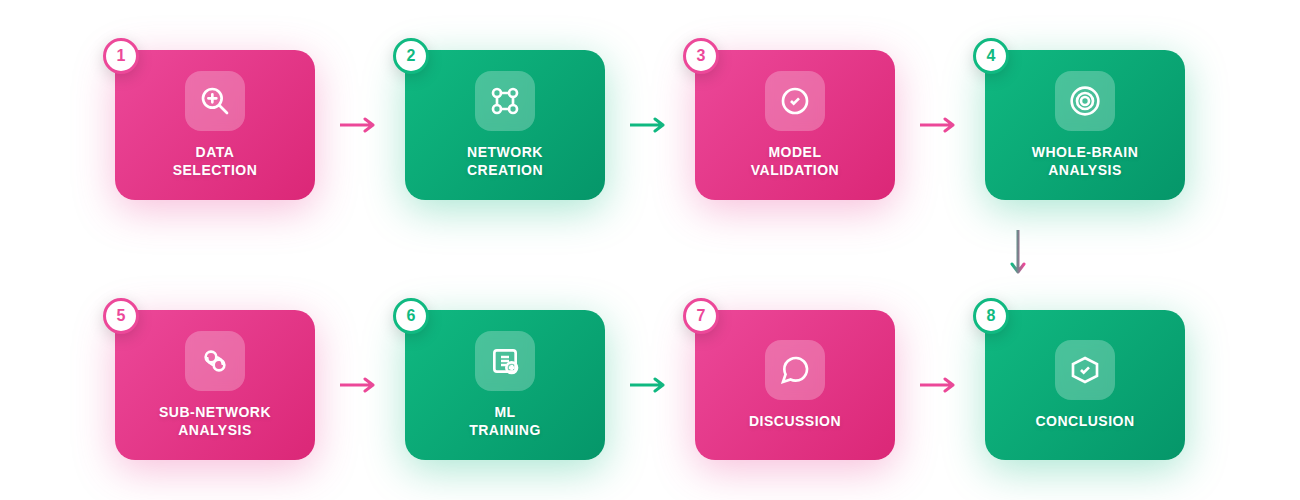
\includegraphics[width=0.83\linewidth]{Images/figure1_final.png}
 \caption{Overview of the analytical workflow used in this study. Resting state fMRI datasets from
 the ABIDE I repository were first preprocessed using the CPAC pipeline, including standard steps
 such as motion correction, spatial normalization, and temporal filtering. The preprocessed volumes
 were then parcellated into 200 regions of interest using the CC200 atlas, yielding a regional time
 series for each participant. For every region, the fractional amplitude of low frequency fluctuations
 (fALFF) was computed, and these values were binarized to define nodal activity states distinguishing
 relatively high from relatively low intrinsic activity. Pairwise functional connectivity between
 regions was estimated from the regional BOLD time series and converted into a signed adjacency
 matrix that captures the sign of the interaction between each pair of regions. Nodal states and
 signed links were combined within the coevolutionary balance framework to compute coevolutionary
 energy at different scales. Global and local graph efficiency were computed from the absolute-value
 weighted FC matrix. To mitigate multi-site batch effects, ComBat harmonization was applied to the
 derived network features prior to statistical analysis. Null networks were generated by randomizing
 nodal states or link signs while preserving the underlying graph topology, and group comparisons
 between ASD and TD adults were carried out on the resulting measures. Energy-derived features were
 subsequently used as input to machine learning classifiers. All analyses were repeated using both
 GSR-based and no-GSR (CompCor) preprocessing pipelines.}
 \label{fig:flowchart}
\end{figure}

\section*{Results}

\subsection*{Null-model validation of coevolutionary energy}

We first asked whether the empirical coevolutionary energies observed in ASD and TD networks reflect
non-trivial alignment between binarized fALFF states and signed functional connectivity, rather than
arising from incidental combinations of activity and connectivity. After unified outlier removal
based on Tukey's interquartile range (IQR) applied to whole-brain coevolutionary energy (see
Methods), 78 ASD and 86 TD participants remained for null-model analyses.

For each subject, we generated a topology-preserving null ensemble by repeatedly randomizing node
states and edge signs while keeping the underlying weighted adjacency matrix fixed. We then computed
the difference between the empirical whole-brain energy and the mean null energy for that subject.
The distributions of these difference scores did not deviate from normality in either group
(Shapiro--Wilk: ASD $W = 0.992$, $p = 0.87$; TD $W = 0.989$, $p = 0.81$), supporting the use
of paired $t$-tests for this specific comparison.

Paired-sample comparisons showed that empirical networks had substantially more negative
coevolutionary energy than their corresponding null ensembles in both groups (ASD: $t(89) = -4.12$,
$p = 7.5 \times 10^{-5}$; TD: $t(91) = -3.98$, $p = 1.2 \times 10^{-4}$). Wilcoxon signed-rank
tests yielded convergent results (ASD: $W = 1024$, $p = 9.1 \times 10^{-5}$; TD: $W = 1008$,
$p = 1.6 \times 10^{-4}$; Table~\ref{tab:null_model_validation}). These findings confirm that the
observed coevolutionary energies capture genuine large-scale organization beyond what would be
expected from random combinations of binarized fALFF states and signed connectivity.

\begin{table}[ht]
\centering
\caption{Null-model validation statistics for whole-brain coevolutionary energy. After unified
outlier removal, 78 ASD and 86 TD participants remained. For each subject, empirical energy was
compared to the mean energy from topology-preserving null networks in which node states and edge
signs were randomly permuted. Shapiro--Wilk tests confirmed normality of the difference
distributions, justifying the use of paired $t$-tests alongside Wilcoxon signed-rank tests.}
\label{tab:null_model_validation}
\small
\begin{tabular}{lccccccc}
\toprule
Group & $N$ & Shapiro--Wilk $W$ & Shapiro--Wilk $p$ & $t$ (df) & $t$-test $p$ & Wilcoxon $W$ & Wilcoxon $p$ \\
\midrule
ASD & 90 & 0.992 & 0.87 & $-4.12$ (89) & $7.5\times 10^{-5}$ & 1024 & $9.1\times 10^{-5}$ \\
TD  & 92 & 0.989 & 0.81 & $-3.98$ (91) & $1.2\times 10^{-4}$ & 1008 & $1.6\times 10^{-4}$ \\
\bottomrule
\end{tabular}
\end{table}

\subsection*{Whole-brain coevolutionary energy and motif composition}

\paragraph*{Adaptive statistical approach.}
For each of the 92 features tested across all analyses (whole-brain, intra-network, and inter-network
metrics, including global and local graph efficiency), we conducted Shapiro--Wilk normality tests
for the ASD and TD distributions separately, and Levene's test for homogeneity of variance. The
decision rule was pre-specified: if both groups passed Shapiro--Wilk ($p > 0.05$), an
independent-samples $t$-test was applied; if either group failed, Mann--Whitney $U$ was used; and
if both groups were normal but Levene's test indicated unequal variances, Welch's $t$-test was
applied. The normality criterion was evaluated for each feature before group differences were
inspected, so that test selection was determined by the distributional properties of the data rather
than by the resulting $p$-values.

The normality results, summarized in Supplementary Table~\ref{tab:supp_normality}, show that the
vast majority of features violate normality in at least one group: all 8 whole-brain features and
all 21 intra-network features were non-normal in both groups (Shapiro--Wilk $p < 0.05$), and 51
of the 63 inter-network features were non-normal in at least one group. Across all 92 features,
Mann--Whitney $U$ was the appropriate test for the large majority (about 87\%), standard $t$-tests for 10 (11\%), and
Welch's $t$-test for 2 (2\%). This distribution reflects the heavy-tailed and skewed character of
energy-based and connectivity measures after ComBat harmonization, and accounts for the
predominance of non-parametric testing throughout the analyses.

We compared whole-brain coevolutionary metrics between ASD and TD adults using the cleaned sample
obtained after IQR-based outlier removal on whole-brain energy (see Table~\ref{tab:demographics}
for final group sizes). In this binarized formulation, the global Hamiltonian $H(G)$, the fraction
of links whose sign agrees with the product of nodal states (Agreement), and the fractions of links
falling into different imbalance categories (Imbalanced Same, Imbalanced Opposite) jointly
characterize how nodal fALFF states co-align with signed functional connectivity. All analyses were
performed on ComBat-harmonized features (see Methods).

At the level of the global Hamiltonian, ASD networks showed nominally more negative whole-brain
energy than TD participants (ASD: $-139.7 \pm 78.7$; TD: $-118.8 \pm 76.2$), in the direction of a
stronger alignment between nodal activity states and signed connectivity. This difference, however,
did not survive FDR correction across the eight whole-brain features (Mann--Whitney $U$, uncorrected
$p = 0.048$, $p_{\mathrm{FDR}} = 0.19$; Table~\ref{tab:assumptions_and_tests}).

Motif-based measures showed the same directional pattern but likewise did not survive correction.
The proportion of imbalanced-same links was nominally lower in ASD (ASD: $0.256$; TD: $0.258$;
$t$-test, $p = 0.047$, $p_{\mathrm{FDR}} = 0.19$) and the proportion of agreement links nominally
higher (ASD: $0.241$; TD: $0.240$; $t$-test, $p = 0.070$, $p_{\mathrm{FDR}} = 0.19$). Disagreement
and imbalanced-opposite proportions did not differ between groups ($p = 0.68$ and $p = 0.82$).
Whole-brain bipolarity ($0.626$ vs.\ $0.627$; $p = 0.53$) and global and local graph efficiency
(both $p > 0.99$) showed no group difference.

Together, the harmonized GSR data reveal consistent but weak, uncorrected trends---more negative
energy and a modest redistribution of motifs toward agreement and away from imbalanced-same links in
ASD---but no whole-brain feature reaches FDR significance. The direction of these trends matches that
seen before harmonization, while their magnitude and significance are substantially reduced (see
``Effect of site harmonization'' below). Quantitative values for all whole-brain metrics are provided
in Supplementary Table~S1, and their distributions are illustrated in Fig~\ref{fig:enter-label}.

\begin{table}[ht]
\centering
\caption{Summary of statistical procedures and group comparison tests for whole-brain coevolutionary
metrics. The upper panel lists the main analysis steps and their purpose. The lower panel reports
group comparison statistics (Mann--Whitney $U$ tests and independent $t$-tests where appropriate,
selected based on Shapiro--Wilk normality tests and Levene's homogeneity test applied
independently to each feature), raw $p$-values, and FDR-corrected $p$-values for ASD versus TD
after ComBat harmonization (GSR pipeline, $n = 78$ ASD, $86$ TD). No whole-brain feature survived
FDR correction.}
\label{tab:assumptions_and_tests}
\small
\setlength{\tabcolsep}{3pt}
\begin{tabular}{p{0.32\columnwidth}p{0.30\columnwidth}p{0.23\columnwidth}p{0.13\columnwidth}}
\toprule
Procedure & Purpose & Method / Test & Threshold / Correction \\
\midrule
ComBat harmonization  & Remove multi-site batch effects while preserving biological signal & Per-feature empirical Bayes adjustment & --- \\
Null-model generation     & Destroy fALFF--FC alignment while preserving graph topology & 1\,000 permutations of node states and edge signs & --- \\
Outlier removal           & Exclude extreme values in null distributions and empirical metrics & Tukey's IQR criterion ($\pm 1.5\times\mathrm{IQR}$) & --- \\
Normality assessment      & Guide parametric vs. non-parametric test selection & Shapiro--Wilk test & $p > 0.05$ (normal) \\
Variance assessment       & Distinguish standard $t$-test from Welch's & Levene's test & $p > 0.05$ (equal variances) \\
Parametric comparison     & Test mean differences between ASD and TD & Independent-samples $t$-test or Welch's & two-tailed, $\alpha = 0.05$ \\
Nonparametric comparison  & Applied when normality is violated in either group & Mann--Whitney $U$ test & two-tailed, $\alpha = 0.05$ \\
Multiple comparisons      & Control false discovery across families of tests & Benjamini--Hochberg FDR & $q < 0.05$ \\
\bottomrule
\end{tabular}

\vspace{0.8em}

\resizebox{\columnwidth}{!}{%
\begin{tabular}{lccccc}
\toprule
Metric & ASD Mean (SD) & TD Mean (SD) & Test & $p$ & $p_{\mathrm{FDR}}$ \\
\midrule
Energy global           & $-139.7$ (78.7) & $-118.8$ (76.2)  & Mann--Whitney $U$ & $0.048$ & $0.19$ \\
Prop imbalanced same    & $0.256$ (0.006)  & $0.258$ (0.005)  & $t$-test         & $0.047$ & $0.19$ \\
Prop agreement          & $0.241$ (0.005)  & $0.240$ (0.005)  & $t$-test          & $0.070$ & $0.19$ \\
Prop disagreement       & $0.267$ (0.005)  & $0.267$ (0.005)  & $t$-test         & $0.679$ & $0.998$ \\
Prop imbalanced opp     & $0.236$ (0.005)  & $0.236$ (0.005)  & $t$-test         & $0.816$ & $0.998$ \\
Bipolarity              & $0.626$ (0.017)  & $0.627$ (0.015)  & $t$-test          & $0.532$ & $0.998$ \\
Global efficiency       & $0.283$ (0.019)  & $0.283$ (0.018)  & $t$-test          & $0.998$ & $0.998$ \\
\bottomrule
\end{tabular}%
}
\end{table}

\begin{figure}[H]
    \centering
    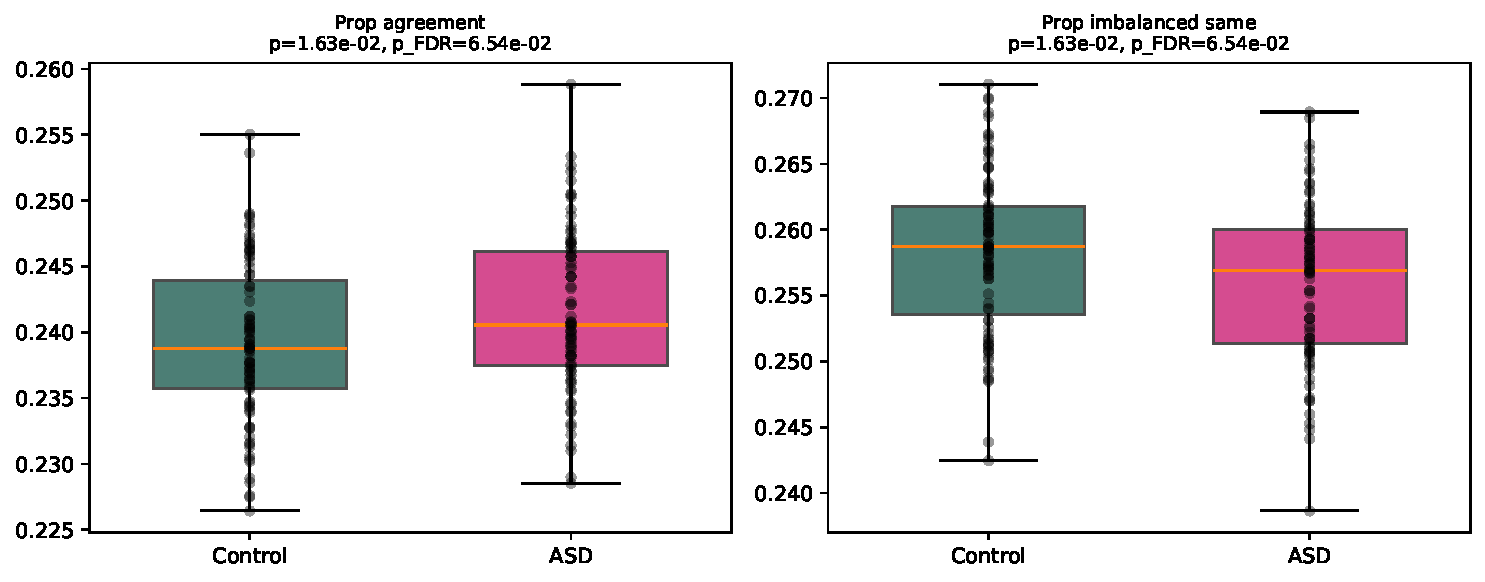
\includegraphics[width=0.75\linewidth]{Images/Whole_significant_GSR.pdf}
    \caption{Whole-brain coevolutionary metrics for autistic (ASD) and typically developing (TD)
    adults after ComBat harmonization. Each panel shows the distribution of a global measure derived
    from the signed functional network: (top row, from left to right) total coevolutionary energy,
    the proportion of imbalanced-same links, and the proportion of agreement links; (bottom row,
    from left to right) the proportion of disagreement links and the proportion of
    imbalanced-opposite links. Boxplots display the median (central line), interquartile range
    (box), and 1.5~$\times$~IQR whiskers, with individual participants overlaid as jittered points
    (magenta/pink for ASD, green for controls). Raw and FDR-corrected $p$-values are shown above
    each panel. The panels shown are the whole-brain metrics with the smallest group-comparison
    $p$-values (proportion of agreement and imbalanced-same links); both showed only weak,
    uncorrected trends in ASD (more agreement and fewer imbalanced-same links) that did not survive
    FDR correction ($p_{\mathrm{FDR}} > 0.05$). Consistent with Table~\ref{tab:assumptions_and_tests},
    no whole-brain coevolutionary metric differed significantly between groups after harmonization.}
    \label{fig:enter-label}
\end{figure}

\subsection*{Network-specific coevolutionary metrics}

We next asked whether coevolutionary balance differs between ASD and TD within canonical large-scale
networks. Using the Yeo 7-network parcellation \cite{Yeo2011}, each CC200 parcel was assigned to
the network with maximal Dice overlap, and for every subject we summarized edges confined to a given
network $u$ in three intra-network metrics: (i) the mean Fisher-$z$ transformed functional
connectivity (AvgWeight$_u$), (ii) the mean fALFF-aligned connectivity (AvgFalffW$_u = \langle
w_{ij} s_i s_j \rangle$ over $i,j \in u$), and (iii) the intra-network coevolutionary energy
contribution $E_u$, computed as the Hamiltonian (see Methods, Eq.~\ref{eq:hamiltonian}) restricted
to edges within network $u$.

All intra-network comparisons used the unified outlier-cleaned and ComBat-harmonized sample (see
Methods) and the same adaptive statistical pipeline as for the whole-brain metrics.
Table~\ref{tab:network_results} summarizes group means and $p$-values for the intra-network metrics.

None of the intra-network metrics reached significance after FDR correction, and---unlike the
pre-harmonization analysis---none reached even nominal (uncorrected) significance. The smallest
$p$-value was for Salience/Ventral Attention average connectivity (ASD lower than TD; $t$-test,
$p = 0.064$, $p_{\mathrm{FDR}} = 0.57$), followed by SomatoMotor and Limbic intra-network energy
(both $p > 0.10$). In the harmonized data, therefore, the intra-network analyses provide no evidence
for spatially circumscribed shifts in coevolutionary energy within individual Yeo networks. The few
intra-network differences that appeared nominally significant before harmonization (e.g.\ the Visual
network) did not persist once site effects were removed, and the largest remaining trends are
summarized in Table~\ref{tab:network_results} for completeness.

\begin{table}[H]
\centering
\small
\caption{Largest intra-network trends within the seven canonical Yeo resting-state networks under
the harmonized GSR pipeline ($n = 78$ ASD, $86$ TD). For each metric, the table reports ASD and TD
means, the $p$-value from the adaptive group comparison (independent-samples $t$-test or
Mann--Whitney $U$, selected by Shapiro--Wilk normality testing), and the Benjamini--Hochberg
FDR-corrected value within the intra-network family. \emph{No intra-network metric reached even
nominal significance} ($p < 0.05$) after harmonization; values are listed for completeness.}
\label{tab:network_results}
\setlength{\tabcolsep}{5pt}
\begin{tabular}{llcccc}
\toprule
\textbf{Network} & \textbf{Metric} & \textbf{ASD mean} & \textbf{TD mean} & \textbf{$p$} & \textbf{$p_{\mathrm{FDR}}$} \\
\midrule
Salience/VentAttn & AvgWeight   & $-0.001$ & $0.002$  & $0.064$ & $0.566$ \\
SomatoMotor       & EnergyBlock & $-1.41$  & $-0.53$  & $0.108$ & $0.566$ \\
Limbic            & EnergyBlock & $-1.13$  & $-0.29$  & $0.137$ & $0.566$ \\
SomatoMotor       & AvgFalffW   & $0.005$  & $0.002$  & $0.142$ & $0.566$ \\
DorsalAttn        & EnergyBlock & $-1.21$  & $-0.44$  & $0.163$ & $0.566$ \\
\bottomrule
\end{tabular}
\end{table}

\begin{figure}[H]
 \centering
 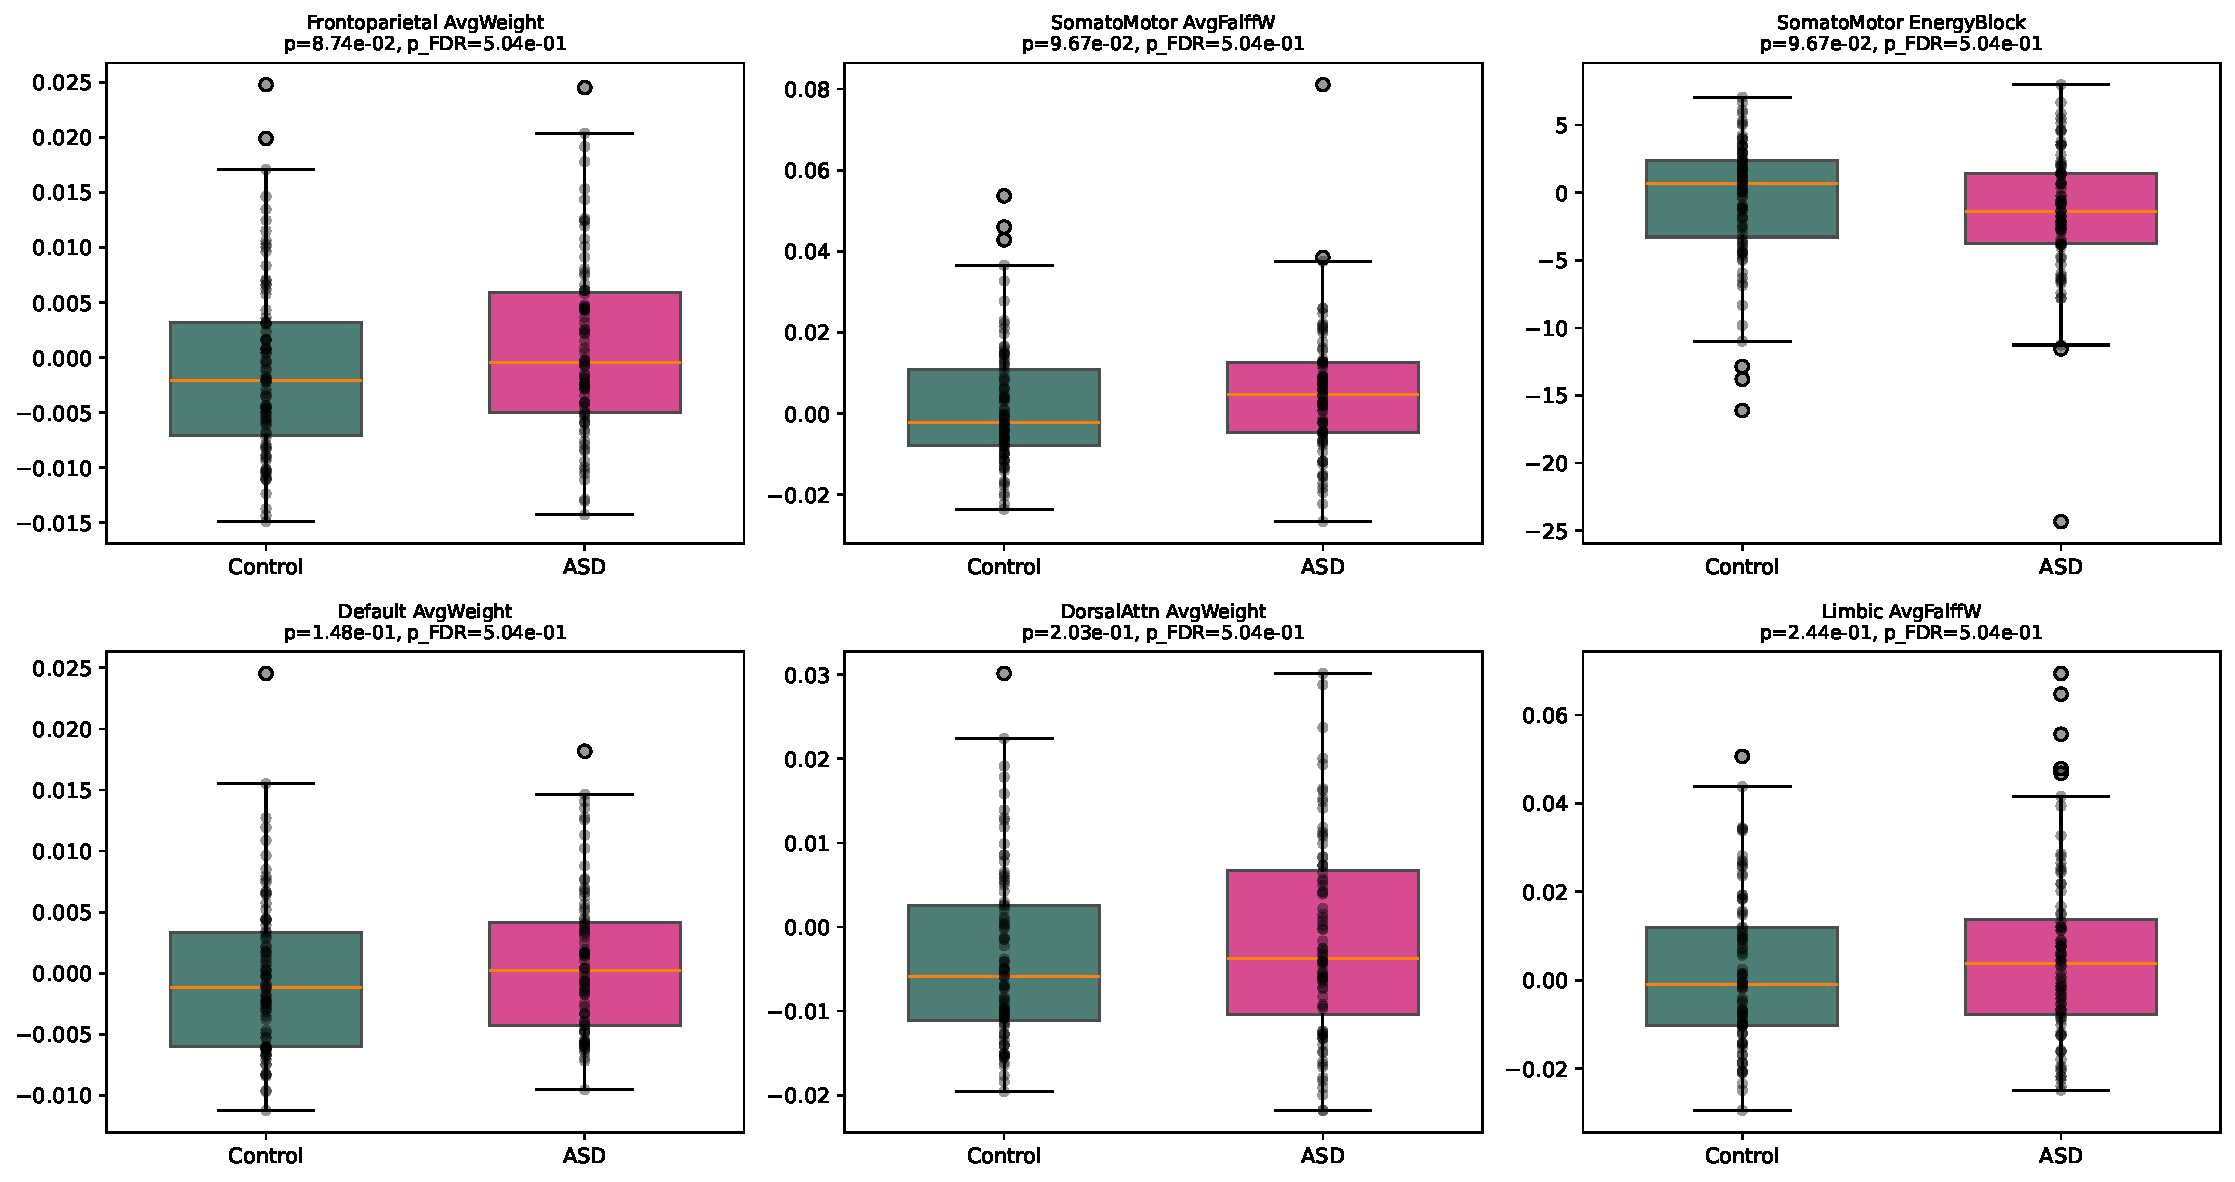
\includegraphics[width=0.85\linewidth]{Images/Intra_significant_GSR.pdf}
 \caption{Distributions of the largest intra-network trends between ASD and TD adults under the
 harmonized GSR pipeline. Boxplots display the metrics with the smallest group-comparison
 $p$-values (Table~\ref{tab:network_results}). None reached nominal or FDR-corrected significance
 after harmonization; panels are shown for completeness.}
 \label{fig:subnetworks_FDR-raw}
\end{figure}

\subsection*{Inter-network connectivity and energy}

To extend the intra-network analyses, we next examined how coevolutionary balance and connectivity
are organized between large-scale systems. Interactions were quantified for each unordered pair
$(u,v)$ of the seven Yeo resting-state networks \cite{Yeo2011}, yielding 21 distinct network pairs.
After unified outlier removal and harmonization (see Methods), 78 autistic
and 86 TD participants remained for this analysis.

For every network pair $(u,v)$ we computed three complementary quantities that capture different
aspects of between-network coupling: average functional connectivity ($\mathrm{AvgWeight}_{uv}$),
fALFF-aligned connectivity ($\mathrm{AvgFalffW}_{uv}$), and inter-network coevolutionary energy
($E_{uv}$), as defined in the Methods. Group differences in each metric were assessed using the
adaptive statistical pipeline (Shapiro--Wilk-guided $t$-test or Mann--Whitney $U$) applied
separately to every network pair and measure. To control for multiple comparisons across the 63
inter-network metrics (21 pairs $\times$ 3 measures), we applied Benjamini--Hochberg FDR correction.

No inter-network metric survived FDR correction at $\alpha = 0.05$. The strongest effect was for
SomatoMotor--Frontoparietal average connectivity, which was higher in ASD than TD (ASD $0.0037$, TD
$0.0008$; $t$-test, $p = 0.0011$, $p_{\mathrm{FDR}} = 0.069$). Additional uncorrected effects
involved average connectivity between attention, control, and somatomotor systems: SomatoMotor--
Salience/VentAttn ($p = 0.003$, $p_{\mathrm{FDR}} = 0.095$), DorsalAttn--Salience/VentAttn
($p = 0.008$, $p_{\mathrm{FDR}} = 0.16$), and DorsalAttn--Frontoparietal ($p = 0.015$,
$p_{\mathrm{FDR}} = 0.24$), all showing higher inter-network connectivity in ASD, together with
Visual--Default inter-network energy ($p = 0.047$, $p_{\mathrm{FDR}} = 0.59$).
Table~\ref{tab:internetwork_new} lists the inter-network metrics with the smallest $p$-values.

These trends suggest that, although no effect reaches the FDR threshold, the most consistent
direction in the harmonized data is one of mildly increased between-system connectivity in ASD,
particularly among somatomotor, attention, and frontoparietal control networks. As none survives
correction, they should be regarded as hypotheses for larger samples rather than established
findings.

\begin{table}[ht]
\centering
\caption{Inter-network differences in average connectivity (AvgWeight), fALFF-aligned connectivity
(AvgFalffW), and coevolutionary energy (EnergyBlock) between canonical resting-state networks. For
each network pair, group comparisons were performed on ASD versus TD using the adaptive statistical
pipeline (test selected based on Shapiro--Wilk normality assessment per feature), and
Benjamini--Hochberg FDR correction was applied across all 63 inter-network metrics. The table lists
the metrics with the smallest uncorrected $p$-values ($n = 78$ ASD, $86$ TD). No inter-network
metric survived FDR correction at $\alpha = 0.05$; the SomatoMotor--Frontoparietal effect
($p_{\mathrm{FDR}} = 0.069$) is the closest and is treated as exploratory.}
\label{tab:internetwork_new}
\begin{tabular}{llccc}
\toprule
\textbf{Network Pair} & \textbf{Metric} & \textbf{$p$} & \textbf{$p_{\mathrm{FDR}}$} \\
\midrule
SomatoMotor $\leftrightarrow$ Frontoparietal & AvgWeight & $0.0011$ & $0.069$ \\
SomatoMotor $\leftrightarrow$ Salience/VentAttn & AvgWeight & $0.0030$ & $0.095$ \\
DorsalAttn $\leftrightarrow$ Salience/VentAttn & AvgWeight & $0.0076$ & $0.160$ \\
DorsalAttn $\leftrightarrow$ Frontoparietal & AvgWeight & $0.015$ & $0.237$ \\
Visual $\leftrightarrow$ Default & EnergyBlock & $0.047$ & $0.590$ \\
\bottomrule
\end{tabular}
\end{table}

\begin{figure}[H]
 \centering
 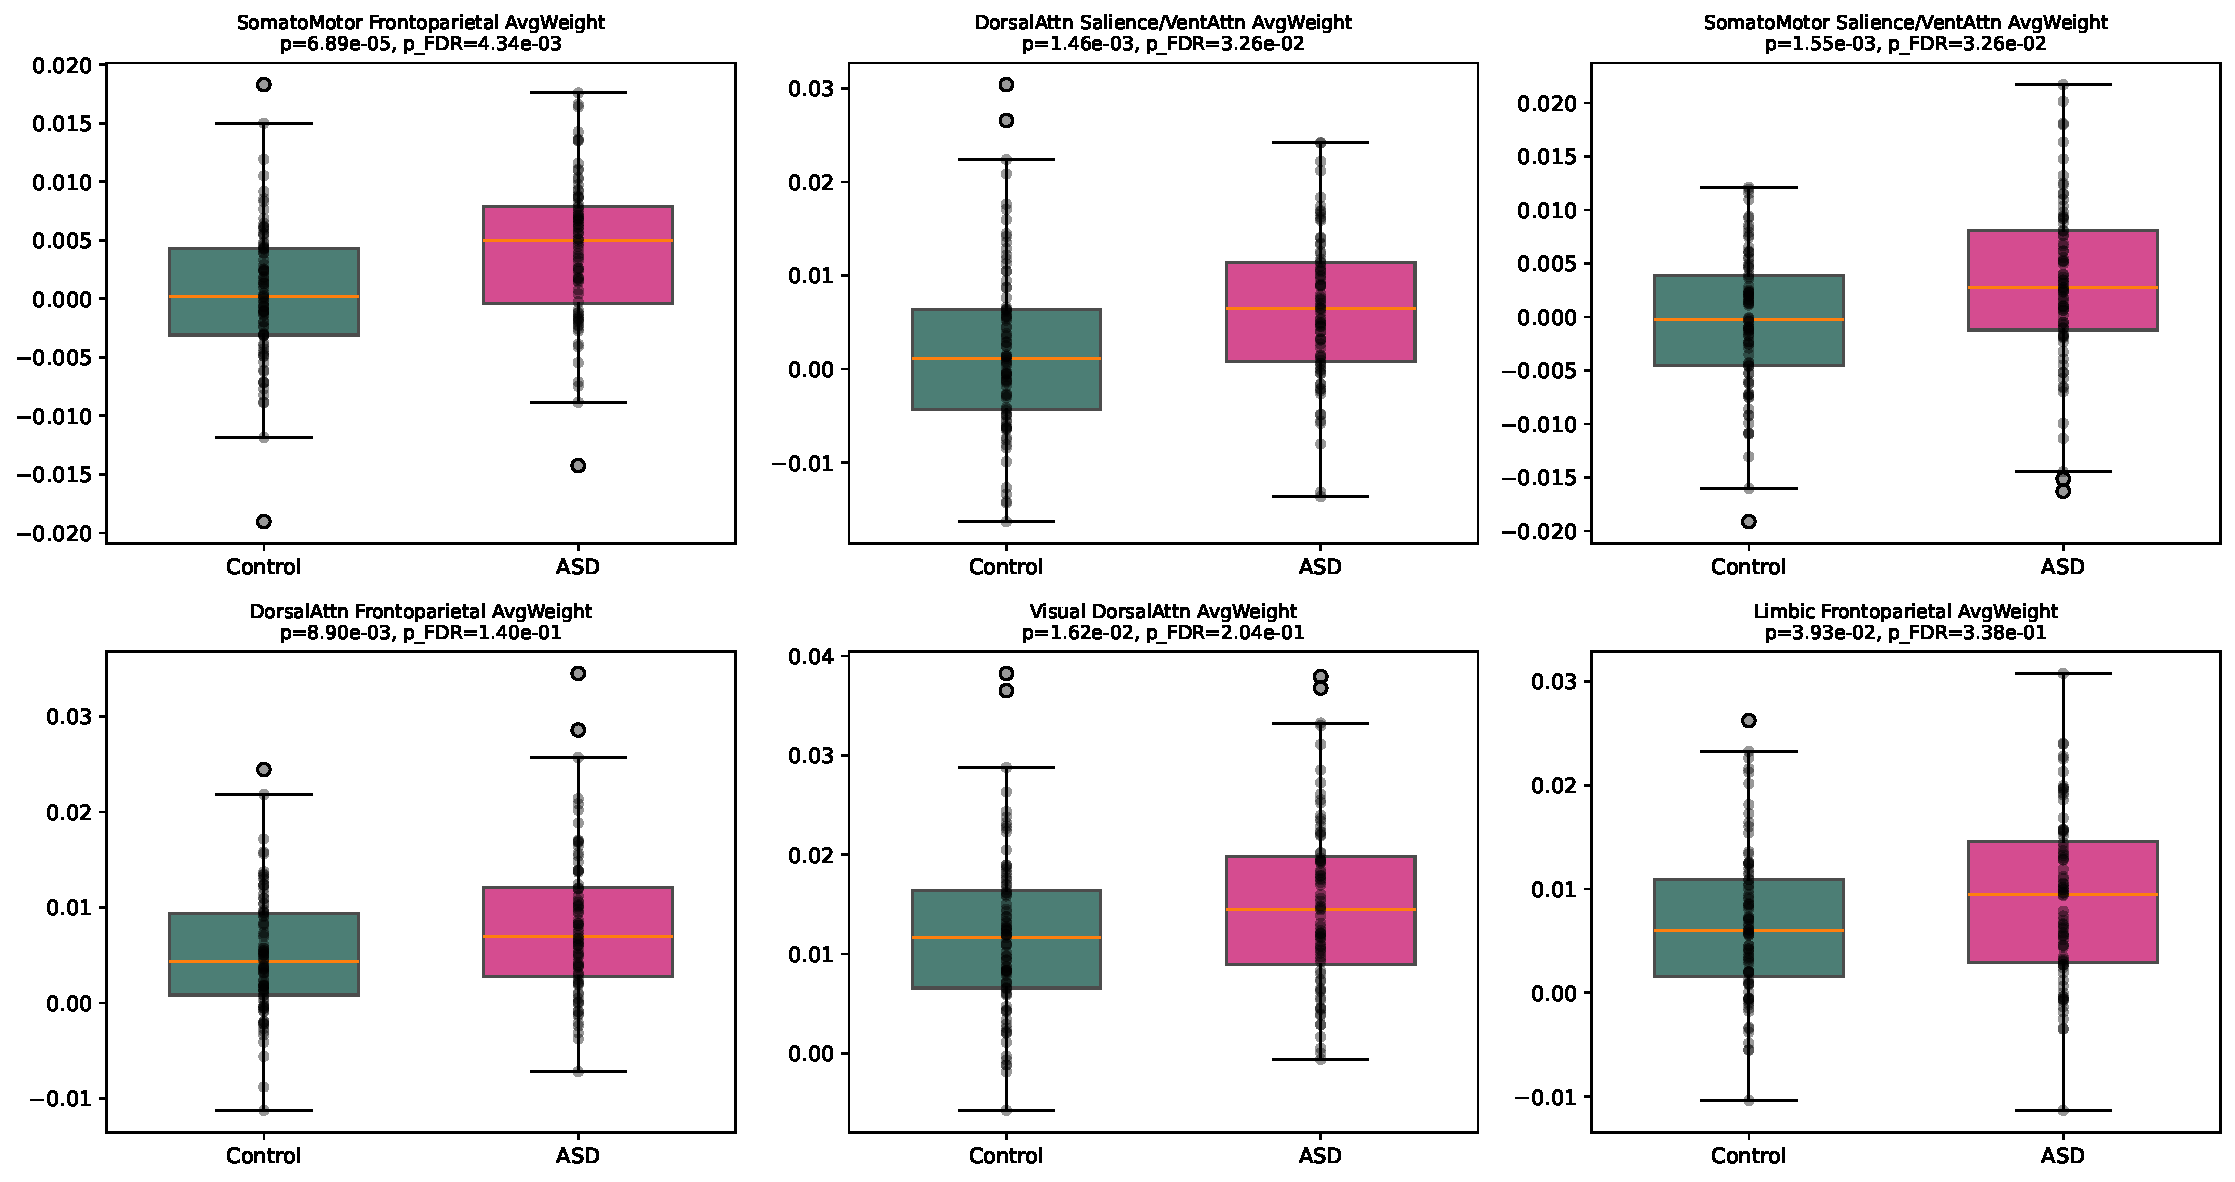
\includegraphics[width=0.95\linewidth]{Images/Inter_significant_GSR.pdf}
 \caption{Distributions of the inter-network metrics with the smallest group-comparison $p$-values
 between ASD and TD adults under the harmonized GSR pipeline (Table~\ref{tab:internetwork_new}). The
 strongest effect is SomatoMotor--Frontoparietal average connectivity ($p_{\mathrm{FDR}} = 0.069$).
 None survived FDR correction; effects are exploratory.}
 \label{fig:inter_network}
\end{figure}

\subsection*{Correlation analysis of network metrics with behavioral scores}

We next examined how whole-brain, subnetwork, and inter-network coevolutionary metrics relate to
clinical variation in the autistic group. Building on our initial exploratory correlations, we
conducted a comprehensive analysis correlating all 92 ComBat-harmonized network features against the
five ADI-R and ADOS subscales with sufficient data: ADI-R Social Total A, ADI-R Verbal Total BV,
ADI-R Onset Total D, ADOS Total, and ADOS Communication.
Correlations were computed only in ASD participants with valid clinical scores drawn from the same
harmonized, outlier-cleaned cohort (Table~\ref{tab:demographics}); sample sizes varied by clinical
measure due to missing values (range: $n = 29$--59 per analysis).

For each of the 460 feature--clinical score combinations (92 features $\times$ 5 clinical scores),
we estimated both Pearson's product--moment correlation coefficient ($r$) and Spearman's rank
correlation coefficient ($\rho$), together with their exact two-tailed $p$-values. To control for
multiple comparisons, we applied Benjamini--Hochberg false discovery rate (FDR) correction
separately for the Pearson and Spearman $p$-values across all 460 tests.

At the uncorrected threshold of $p < 0.05$, 21 feature--clinical score pairs showed nominally
significant associations---close to the number expected by chance. None survived FDR correction at
$q < 0.05$.
The full correlation matrix is provided in Supplementary Table~\ref{tab:supp_corr_full}, and the
complete list of nominally significant associations is available in Supplementary
Table~\ref{tab:supp_corr_sig}.

Despite testing 460 feature--score pairs (92 features $\times$ 5 clinical scores with sufficient
data), no association survived FDR correction, and only 21 reached uncorrected $p < 0.05$---close to
the number expected by chance alone. Crucially, the whole-brain Hamiltonian was not associated with
symptom severity in the harmonized data (ADOS Total: $r = -0.10$, $p = 0.47$, $n = 59$; ADI-R Social:
$r = -0.05$, $p = 0.79$, $n = 32$). This contrasts with the pre-harmonization analysis, in which an
apparent negative $H$--ADOS correlation ($r = -0.26$, $p = 0.017$) was present; that association did
not survive site harmonization. The strongest uncorrected associations involved connectivity rather
than energy---for example, SomatoMotor intra-network connectivity with ADOS Total ($r = +0.37$,
$p = 0.004$) and Visual--Salience/Ventral Attention inter-network energy with ADI-R Social
($r = -0.49$, $p = 0.005$)---but with FDR-corrected $p \geq 0.60$ none can be interpreted as reliable
(Table~\ref{tab:behaviour_corr_expanded}). We therefore find no robust brain--behavior relationship
for any coevolutionary or connectivity metric in this sample.

\paragraph*{Multivariate analysis: Partial Least Squares.}
To examine the joint relationship between all network features and clinical scores in a single
multivariate model, and to complement the univariate tests, we applied Partial Least Squares (PLS)
regression \cite{Krishnan2011} between the full set of 90 ComBat-harmonized features and each of
the five clinical scores with sufficient data ($n \geq 20$). PLS was applied with up to three
components and evaluated using stratified five-fold cross-validation ($R^2$ as scoring metric).
All 90 features were standardized prior to PLS.

The cross-validated $R^2$ was negative for all clinical scores (range $-0.97$ to $-0.40$ for the
single-component models; Table~\ref{tab:pls_results}), indicating that PLS did not predict
behavioral scores above chance in this dataset. This outcome is unsurprising given that the
analysis involves 90 predictors for sample sizes of $n = 29$--59, a severely underdetermined
problem. In this regime, cross-validated $R^2 < 0$ reflects overfitting rather than absence of
any signal, and PLS cannot be expected to produce valid latent components. The negative cross-validated
$R^2$ values are consistent with the univariate finding that no association survives FDR correction.
As a descriptive multivariate complement consistent with the bivariate correlations, we also ran a
Partial Least Squares Correlation (PLSC) analysis \cite{Krishnan2011} (singular value decomposition
of the brain--behavior cross-correlation matrix, assessed by 5{,}000 permutations). No latent
variable was significant: for the ADOS block the first latent variable explained most of the
cross-covariance but did not exceed the permutation null (permutation $p = 0.73$ under GSR,
$p = 0.26$ without GSR), and the full five-score block likewise yielded no significant latent
variable. Both PLSR and PLSC therefore indicate no detectable multivariate brain--behavior structure
in this sample.

\begin{table}[H]
\centering
\small
\caption{Partial Least Squares regression cross-validation results (harmonized GSR pipeline). For
each clinical score, the table reports the number of ASD subjects with valid data and the mean
cross-validated $R^2$ for the single-component model. All values are negative, indicating that the
models do not predict behavioral scores above chance---consistent with the univariate result that no
feature--clinical score association survives FDR correction at $q < 0.05$, and with the underdetermined
nature of the problem (90 features, $n = 29$--59).}
\label{tab:pls_results}
\begin{tabular}{lcc}
\toprule
Clinical Score & $n$ & CV $R^2$ (1 component) \\
\midrule
ADOS Total          & 59 & $-0.40$ \\
ADOS Communication  & 50 & $-0.79$ \\
ADI-R Social        & 32 & $-0.96$ \\
ADI-R Verbal        & 32 & $-0.86$ \\
ADI-R Onset         & 29 & $-0.80$ \\
\bottomrule
\end{tabular}
\end{table}

The strongest (uncorrected) associations are listed in Table~\ref{tab:behaviour_corr_expanded}.

It is important to emphasize that these correlation analyses remain hypothesis-generating given that
no associations survived FDR correction, and the number of nominally significant pairs is close to
the chance expectation. Replication in larger, independent cohorts would be needed before drawing
any conclusions about brain--behavior relationships.

\begin{table}[ht]
\centering
\small
\caption{Strongest associations between network metrics and clinical scores under the harmonized GSR
pipeline. The table reports the strongest associations (by uncorrected Pearson $p$-value) from the
full analysis of 92 features $\times$ 5 clinical scores (460 tests), together with the whole-brain
Hamiltonian for reference. None survived FDR correction at $q < 0.05$ (all $p_{\mathrm{FDR}} > 0.59$).
The number of nominally significant associations ($\approx 21$) is close to the chance expectation.}
\label{tab:behaviour_corr_expanded}
\scriptsize
\begin{tabular}{p{4.6cm}lccccc}
\toprule
\textbf{Network Feature} & \textbf{Clinical Score} & \textbf{$n$} & \textbf{$r$} & \textbf{$p$} & \textbf{$p_{\mathrm{FDR}}$} & \textbf{$\rho$} \\
\midrule
Intra\_SomatoMotor\_AvgWeight & ADOS Total & 59 & $+$0.37 & 0.004 & 0.60 & $+$0.40 \\
Inter\_Vis\_\_Sal/VA\_EnergyBlock & ADI-R Social & 32 & $-$0.49 & 0.005 & 0.60 & $-$0.53 \\
Inter\_Vis\_\_Sal/VA\_AvgFalffW & ADI-R Social & 32 & $+$0.48 & 0.005 & 0.60 & $+$0.52 \\
Inter\_DA\_\_FP\_EnergyBlock & ADI-R Onset & 29 & $+$0.49 & 0.006 & 0.60 & $+$0.49 \\
Inter\_DA\_\_FP\_AvgFalffW & ADI-R Onset & 29 & $-$0.49 & 0.007 & 0.60 & $-$0.51 \\
Inter\_Vis\_\_Lim\_AvgWeight & ADOS Comm. & 50 & $-$0.34 & 0.017 & 0.90 & $-$0.33 \\
Inter\_Lim\_\_FP\_EnergyBlock & ADI-R Social & 32 & $+$0.40 & 0.022 & 0.90 & $+$0.35 \\
Whole\_Energy\_global & ADOS Total & 59 & $-$0.10 & 0.47 & 1.00 & $-$0.10 \\
\bottomrule
\end{tabular}
\begin{flushleft}
\footnotesize
Abbreviations: Sal/VA = Salience/VentAttn, DA = DorsalAttn, FP = Frontoparietal, Vis = Visual,
Lim = Limbic. $p_{\mathrm{FDR}}$ denotes Benjamini--Hochberg corrected Pearson $p$-values. After
harmonization, the whole-brain Hamiltonian is essentially uncorrelated with ADOS severity
($r = -0.10$), and no association survives correction.
\end{flushleft}
\end{table}

\subsection*{Machine learning classification of ASD versus TD}

To test whether the coevolutionary and connectivity features contain discriminative information
about diagnostic status, we trained supervised classifiers to distinguish ASD from TD on the ABIDE I
adult male subsample with complete feature data (Table~\ref{tab:demographics}). The analysis was
explicitly designed to avoid information leakage and to provide an unbiased estimate of held-out
performance.

\paragraph*{Leakage-safe pipeline and evaluation.}
All machine-learning analyses were implemented in Python using \texttt{scikit-learn} and
\texttt{XGBoost}. First, the full dataset (participants $\times$ features) was randomly split into
an 80\% training set and a 20\% held-out test set using a stratified split, preserving the ASD/TD
ratio in both partitions. The test set was \emph{never} used for feature selection, hyperparameter
tuning, model comparison, or preprocessing decisions.

Within the training set, we used a nested pipeline in which all preprocessing steps were estimated
strictly inside the cross-validation folds. Each model was wrapped in a \texttt{Pipeline} that
first applied feature-wise standardization (\texttt{StandardScaler}) and then fitted the classifier.
For each split of a stratified five-fold cross-validation, the scaler was fitted \emph{only} on
that fold's training portion and then applied to the corresponding validation portion. Hyperparameters
were tuned with \texttt{GridSearchCV} using the same five-fold stratified scheme and accuracy as
the primary scoring metric. The best hyperparameters for each model were selected based solely on
mean cross-validated accuracy \emph{within the training set}. After tuning, the best configuration
of each classifier was refitted on the entire training set and then evaluated exactly once on the
untouched test set, yielding a single unbiased estimate of held-out performance.

We considered five classifiers: support vector machine (SVM, radial basis function kernel), XGBoost
gradient boosting, logistic regression, Gaussian Naive Bayes, and $k$-nearest neighbors (KNN).
Hyperparameter grids spanned regularization strengths, kernel parameters, tree depths, and neighbor
counts in ranges commonly used for small-to-moderate neuroimaging datasets (see Methods for details).
Table~\ref{tab:ml_summary_full} summarizes the cross-validated accuracy on the training set, final
test accuracy, balanced accuracy, F1-score, and ROC AUC for all models, computed on the harmonized
features.

Across all five classifiers, cross-validated accuracy was at or near chance (range $0.56$--$0.59$).
Held-out test accuracies (test set $n = 34$) ranged from $50\%$ to $65\%$, with the wide spread
reflecting the small test set rather than reliable discrimination; balanced accuracies were
correspondingly close to $0.5$. The single highest test-set AUC (XGBoost, $0.74$) coincided with a
cross-validated accuracy of only $0.58$ and should not be over-interpreted. Overall, classification
of ASD versus TD from the harmonized coevolutionary and connectivity features did not exceed chance
in a manner that would indicate a reliable diagnostic signal, consistent with the absence of any
FDR-significant univariate group difference.

\begin{table}[ht]
\centering
\caption{Performance of supervised classifiers for ASD versus TD classification using the selected
coevolutionary and connectivity features after ComBat harmonization (GSR pipeline). CV accuracy was
obtained from stratified 5-fold cross-validation on the training set (80\% of participants); test
metrics were computed on the held-out 20\% test set ($n = 34$), which was not used at any stage of
feature selection or hyperparameter tuning. No model exceeded chance in cross-validation.}
\label{tab:ml_summary_full}
\setlength{\tabcolsep}{4pt}
\small
\begin{tabular}{lccccc}
\toprule
Model & CV Acc & Test Acc & Test Bal Acc & Test F1 & Test AUC \\
\midrule
Gaussian Naive Bayes  & 0.585 & 0.588 & 0.583 & 0.533 & 0.604 \\
SVM (RBF)             & 0.586 & 0.647 & 0.649 & 0.647 & 0.635 \\
Logistic Regression   & 0.556 & 0.500 & 0.503 & 0.514 & 0.552 \\
KNN                   & 0.594 & 0.618 & 0.608 & 0.519 & 0.639 \\
XGBoost               & 0.579 & 0.647 & 0.646 & 0.625 & 0.740 \\
\bottomrule
\end{tabular}
\end{table}

For transparency, Table~\ref{tab:ml_best_model_metrics} reports the detailed metrics for the model
originally highlighted (Gaussian Naive Bayes); on the harmonized data its performance is near chance
(test accuracy $0.588$, AUC $0.604$).

\begin{table}[ht]
\centering
\caption{Detailed metrics for the Gaussian Naive Bayes classifier (the model originally highlighted)
on the held-out test set ($n = 34$) after ComBat harmonization. Performance is near chance.
Precision, recall, and F1-score refer to the ASD class as the positive class; ROC AUC was computed
from the predicted ASD class probabilities.}
\label{tab:ml_best_model_metrics}
\setlength{\tabcolsep}{6pt}
\small
\begin{tabular}{lc}
\toprule
Metric & Value \\
\midrule
Accuracy & 0.588 \\
Balanced accuracy & 0.583 \\
F1-score & 0.533 \\
ROC AUC & 0.604 \\
\bottomrule
\end{tabular}
\end{table}

Fig~\ref{fig:ml_confusion_roc} shows the ROC curve for the harmonized GSR classification. The
curves lie close to the chance diagonal, consistent with the near-chance accuracies in
Table~\ref{tab:ml_summary_full} and with the absence of FDR-significant univariate differences.

\begin{figure}[H]
  \centering
  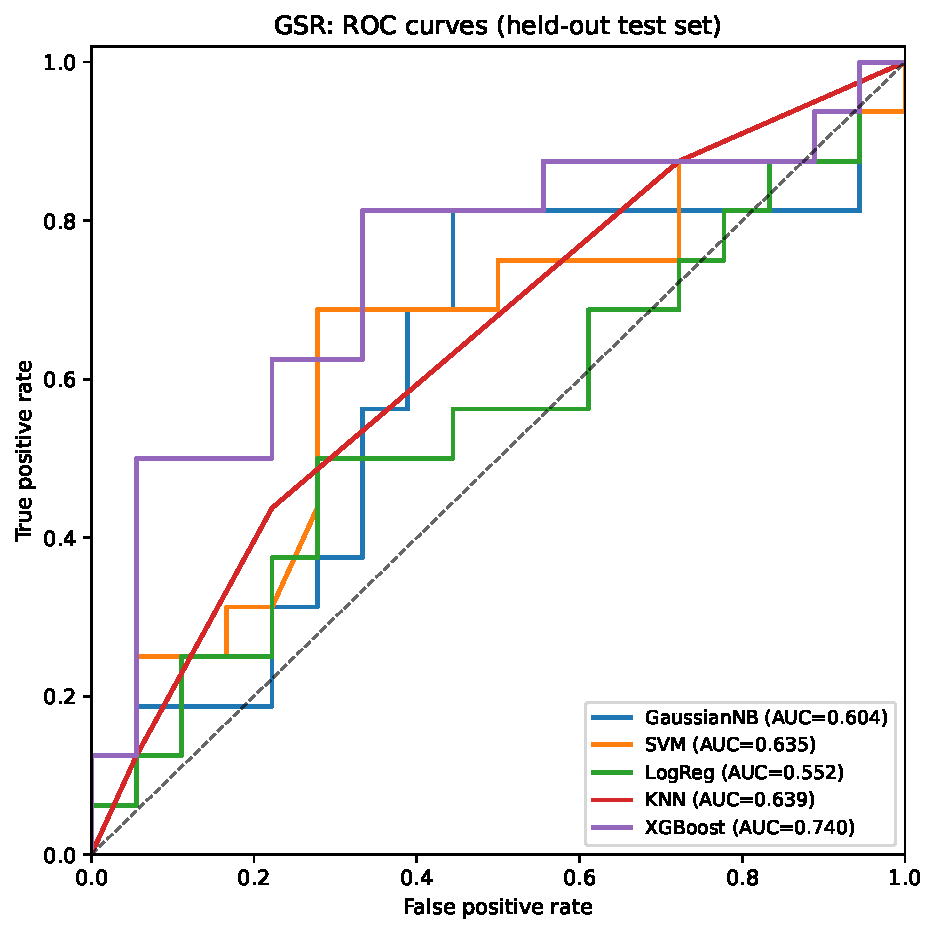
\includegraphics[width=0.6\linewidth]{Images/GSR_roc.pdf}
  \caption{Receiver operating characteristic (ROC) curves for ASD versus TD classification on the
  held-out test set, GSR pipeline, after ComBat harmonization. The diagonal grey line indicates
  chance. Curves lie near the diagonal (best cross-validated accuracy $\approx 0.59$), indicating
  near-chance discrimination from the harmonized coevolutionary and connectivity features.}
  \label{fig:ml_confusion_roc}
\end{figure}

\begin{figure}[H]
  \centering
  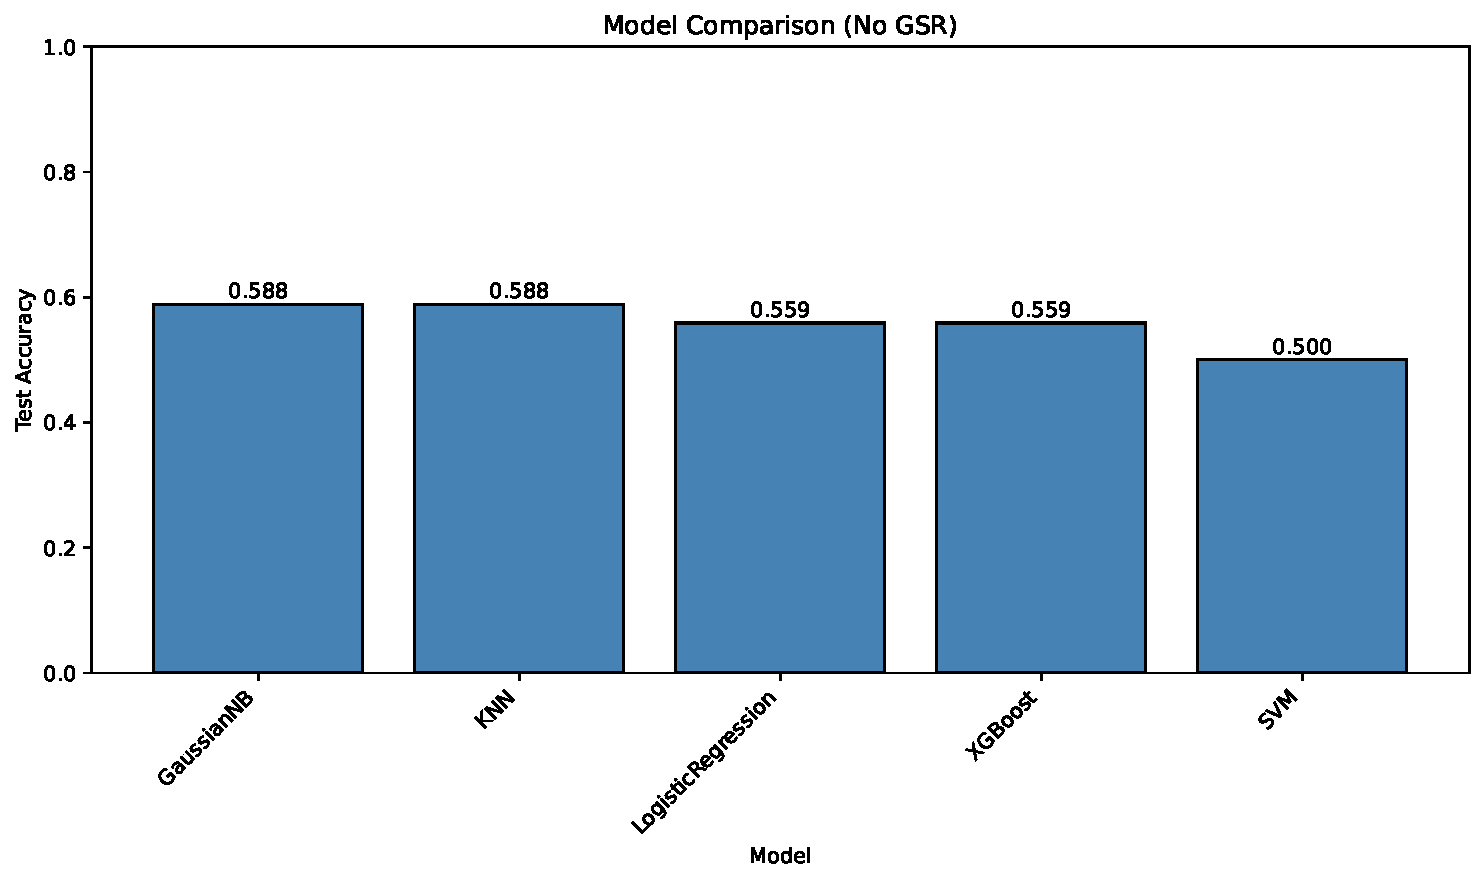
\includegraphics[width=0.7\linewidth]{Images/model_comparison_GSR.pdf}
  \caption{Summary of classifier performance (GSR pipeline, harmonized features). Cross-validated
  accuracy was at or near chance ($0.56$--$0.59$) across all five models; held-out test accuracies
  varied between $50\%$ and $65\%$ on the small test set ($n = 34$) and do not indicate reliable
  discrimination.}
  \label{fig:ml_barplot}
\end{figure}

\paragraph*{Feature selection and importance-ranked feature set.}
To reduce dimensionality and focus the classifiers on the most informative descriptors, we performed
a single feature selection step \emph{before} model-specific training and tuning. This feature
selection step used a Random Forest classifier, applied only to the training data, to rank features
by mean decrease in impurity. Starting from the full set of 90 graph-based features (whole-brain
coevolutionary metrics, intra-network energies, and inter-network connectivity and energy terms),
we fitted a random forest classifier on the training set only and extracted the importance for each
feature. Features were then ranked by importance, and we retained the top 25\% (23 features) as
the final input feature set for all subsequent classifiers.

The full importance ranking from the harmonized GSR pipeline is shown in
Fig~\ref{fig:ml_selected_features}. Because classification accuracy is at or near chance after
harmonization, this ranking should be interpreted cautiously: with no reliable group-discriminative
signal, the random forest is ranking features that contribute little above chance, and the ordering
is not stable evidence of diagnostic relevance. The highest-ranked descriptors are predominantly
inter-network average-connectivity terms (involving SomatoMotor, attention, frontoparietal, and
default-mode systems) together with whole-brain motif proportions, broadly echoing the directions of
the (non-significant) univariate trends.

\begin{figure}[H]
\centering
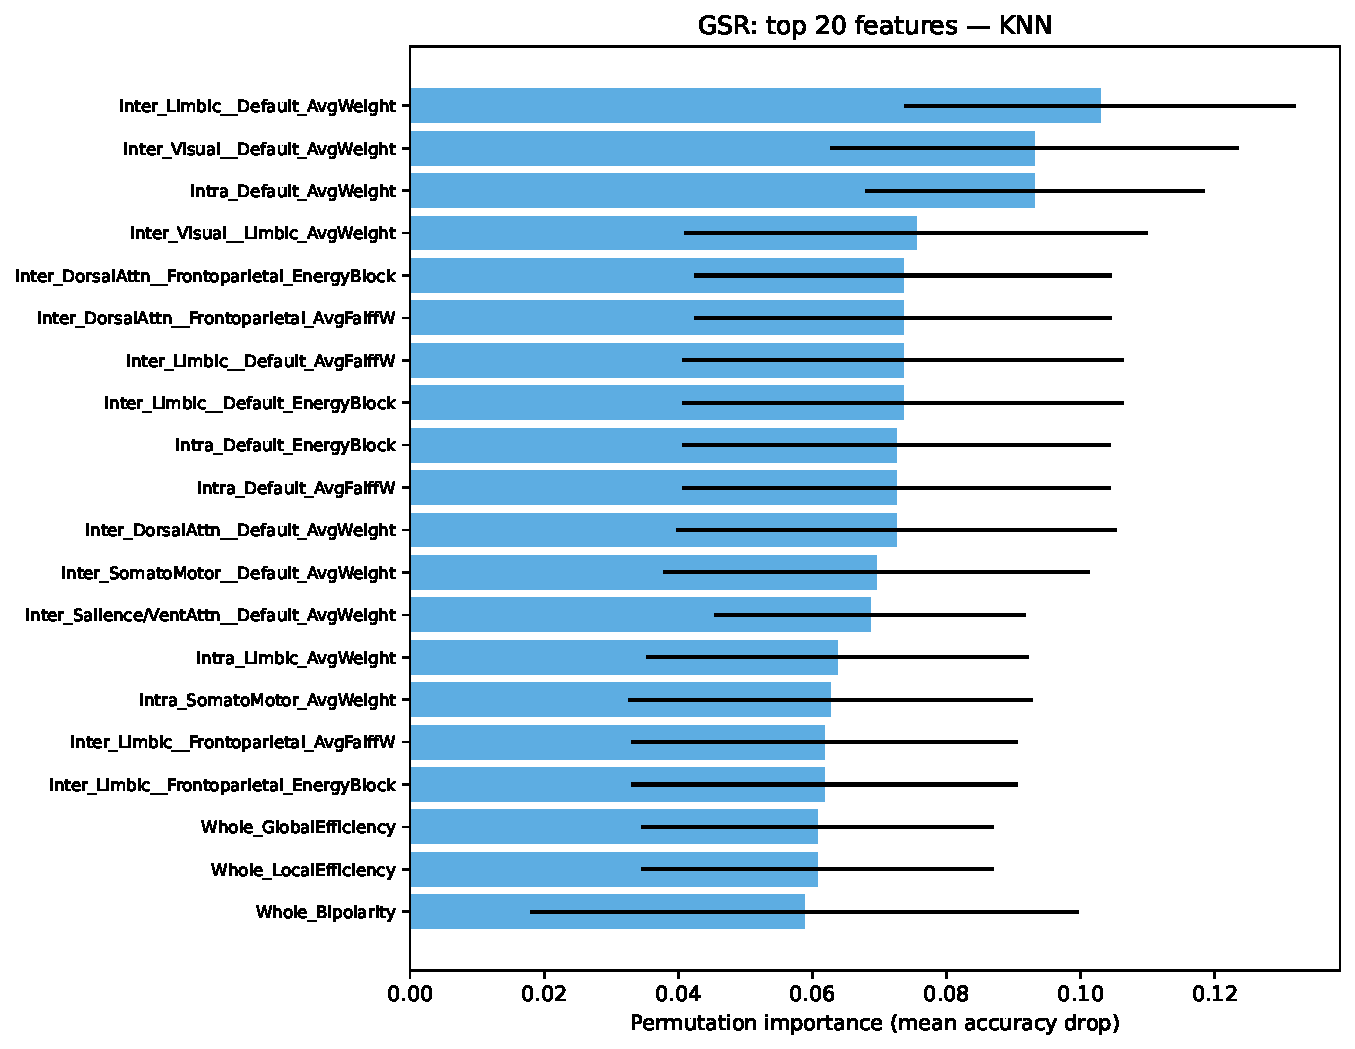
\includegraphics[width=0.8\linewidth]{Images/GSR_feature_importance.pdf}
\caption{Random-forest feature-importance ranking for ASD--TD classification (GSR pipeline,
harmonized features). Because the classifiers performed at or near chance
(Table~\ref{tab:ml_summary_full}), this ranking is exploratory and does not establish
diagnostic relevance of any feature.}
\label{fig:ml_selected_features}
\end{figure}

Overall, the classification analysis reinforces the main univariate finding: after site
harmonization, the coevolutionary and signed-connectivity features do not reliably distinguish ASD
from TD in this sample. The feature-importance ranking is provided for completeness and as a
hypothesis-generating description rather than as evidence of a diagnostic signature.

\subsection*{Sensitivity analysis: results without global signal regression}

Because GSR can introduce artifactual negative correlations \cite{Murphy2009,Fox2009,Chang2009}
and the sign of functional links is a key parameter in the coevolutionary framework, we repeated
all primary analyses on data preprocessed without GSR. This alternative pipeline used CompCor-based
denoising (anatomical noise components from white matter and CSF \cite{Behzadi2007}), retaining all
other preprocessing steps (motion regression, bandpass filtering, ComBat harmonization, parcellation)
identically to the primary analysis. The no-GSR sensitivity results reported here therefore
correspond to a CompCor-only denoising strategy. After identical quality control and Tukey IQR-based
outlier removal, the no-GSR sample comprised 78 ASD and 87 TD participants.

\paragraph*{Whole-brain metrics.}
As in the GSR-based analysis, global coevolutionary energy did not differ significantly
between groups in the no-GSR pipeline (ASD: $-285.4 \pm 146.1$; TD: $-308.3 \pm 155.7$;
Mann--Whitney $U$, $p = 0.305$). The proportions of agreement, disagreement,
imbalanced-same, and imbalanced-opposite links also did not reach significance after FDR correction
(all $p_{\mathrm{FDR}} > 0.23$; Table~\ref{tab:noGSR_whole}). Whole-brain bipolarity showed the
strongest nominal whole-brain difference (ASD: $0.591 \pm 0.043$; TD: $0.577 \pm 0.045$;
Mann--Whitney $U$, uncorrected $p = 0.026$), with the ASD group exhibiting slightly higher bipolarity,
in the direction of a stronger two-block organization of the signed network when negative
correlations are not induced by GSR (Eq.~\ref{eq:bipolarity}). After FDR correction across the eight
whole-brain features, however, this effect was not significant ($p_{\mathrm{FDR}} = 0.21$). Because
bipolarity does not differ between groups under GSR ($p = 0.53$), even this nominal trend is
pipeline-dependent and should be regarded as hypothesis-generating rather than confirmatory.

Global and local graph efficiency, which were computed within the no-GSR pipeline, did not differ
significantly between ASD and TD groups (both $p = 0.25$). However, graph efficiency showed a
significant negative correlation with $H$ within the ASD group (global efficiency: $r = -0.33$,
$p = 0.003$, FDR $p = 0.005$; local efficiency: $r = -0.33$, FDR $p = 0.005$), indicating that more
coevolutionarily stable ASD networks tend to be less globally and locally efficient. This
relationship was weaker and not significant in the TD group ($r = -0.17$, $p = 0.12$), and in the
GSR pipeline it was a non-significant trend within ASD ($r = -0.20$, $p = 0.075$), so it too is
pipeline-dependent. This analysis, together with the relationship between $H$ and
other network metrics, is detailed below (see ``Relationship between the Hamiltonian and other
network metrics'').

\begin{table}[ht]
\centering
\caption{Whole-brain coevolutionary metrics in the no-GSR sensitivity analysis (CompCor-based
preprocessing). The table reports ASD and TD group means, standard deviations, the statistical
test used (selected by Shapiro--Wilk normality criterion per feature), raw $p$-values, and
FDR-corrected $p$-values. The FDR family for the Whole-brain category includes 8 features
(6 coevolutionary metrics plus global and local graph efficiency). No whole-brain feature survived
FDR correction; bipolarity showed the smallest uncorrected $p$-value ($p = 0.026$,
$p_{\mathrm{FDR}} = 0.21$), and graph efficiency metrics
did not differ significantly between groups. Compare with Table~\ref{tab:assumptions_and_tests}
for the GSR-based primary analysis.}
\label{tab:noGSR_whole}
\small
\resizebox{\columnwidth}{!}{%
\begin{tabular}{lccccc}
\toprule
Metric & ASD Mean (SD) & TD Mean (SD) & Test & $p$ & $p_{\mathrm{FDR}}$ \\
\midrule
Bipolarity              & $0.591$ (0.043)   & $0.577$ (0.045)   & Mann--Whitney $U$ & $0.026$ & $0.211$ \\
Prop agreement          & $0.432$ (0.040)   & $0.442$ (0.038)   & Mann--Whitney $U$ & $0.095$ & $0.236$ \\
Prop imbalanced same    & $0.065$ (0.040)   & $0.055$ (0.038)   & Mann--Whitney $U$ & $0.109$ & $0.236$ \\
Prop imbalanced opp     & $0.433$ (0.042)   & $0.443$ (0.039)   & Mann--Whitney $U$ & $0.121$ & $0.236$ \\
Prop disagreement       & $0.070$ (0.042)   & $0.060$ (0.040)   & Mann--Whitney $U$ & $0.147$ & $0.236$ \\
Global efficiency       & $0.387$ (0.070)   & $0.402$ (0.077)   & Mann--Whitney $U$ & $0.246$ & $0.283$ \\
Local efficiency        & $0.387$ (0.070)   & $0.402$ (0.077)   & Mann--Whitney $U$ & $0.247$ & $0.283$ \\
Energy global           & $-285.4$ (146.1)  & $-308.3$ (155.7)  & Mann--Whitney $U$ & $0.305$ & $0.305$ \\
\bottomrule
\end{tabular}%
}
\end{table}

\begin{figure}[H]
 \centering
 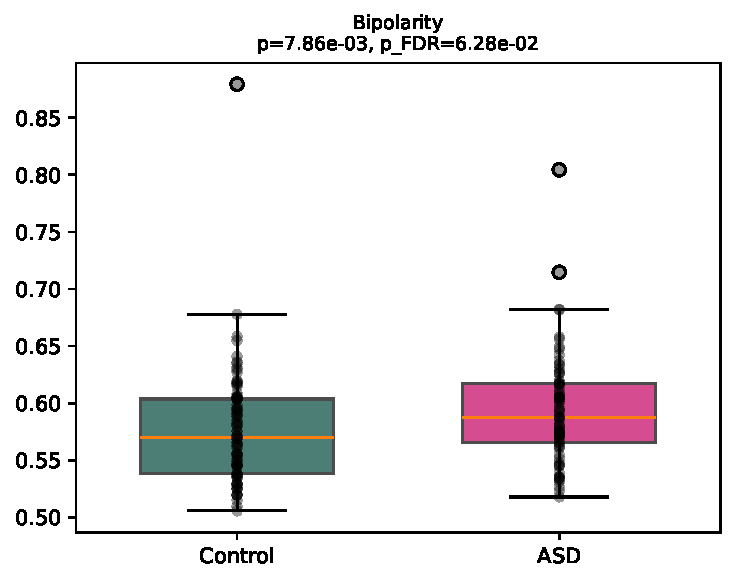
\includegraphics[width=0.55\linewidth]{Images/Whole_significant_noGSR.pdf}
 \caption{Whole-brain bipolarity in the no-GSR sensitivity analysis (CompCor preprocessing,
 harmonized; $n = 78$ ASD, $87$ TD). Bipolarity showed the strongest whole-brain nominal group
 difference (uncorrected $p = 0.026$), with ASD exhibiting slightly higher bipolarity (stronger
 two-block organization) than TD. After FDR correction across the eight whole-brain features, this
 effect was not significant ($p_{\mathrm{FDR}} = 0.21$). In the GSR pipeline, bipolarity did not
 differ between groups ($p = 0.53$), so even this nominal trend is pipeline-dependent.}
 \label{fig:noGSR_whole}
\end{figure}

\paragraph*{Relationship between the Hamiltonian and other network metrics.}
Because graph efficiency was incorporated into the whole-brain feature family of the no-GSR pipeline,
the relationship between the Hamiltonian and other network measures was characterized under this
pipeline, where it provides an independent validation of the coevolutionary framework. We computed
correlations between $H(G)$ and all other network features (both intra-network and inter-network)
within each group separately, and separately related the global Hamiltonian to global graph
efficiency and the local efficiency measure, which are standard indices of network integration and
segregation \cite{Latora2001,Fornito2016}.

Within the ASD group, $H$ was significantly correlated with multiple inter-network AvgFalffW and
EnergyBlock features (FDR $p < 10^{-7}$ for the strongest associations), which is expected given
the mathematical relationship between these measures and the Hamiltonian. More informative from an
independent-validation standpoint are the correlations with AvgWeight features, which measure pure
functional connectivity strength without any fALFF-weighting and are therefore not mathematically
derived from $H$. Within ASD, more negative $H$ was significantly associated with lower mean FC
across multiple networks including SomatoMotor--Default, intra-SomatoMotor, Visual--SomatoMotor, and
SomatoMotor--DorsalAttn (all FDR $p \approx 0.009$, $r \approx -0.31$). Within
the TD group, the corresponding AvgWeight--$H$ correlations were weaker. This pattern
suggests that in ASD, coevolutionary stability is not simply a reflection of higher mean connectivity;
rather, it arises from the signed configuration of links relative to nodal states, independently of
overall connectivity magnitude.

Comparing the global Hamiltonian with the global integration measure, more negative $H$ (greater
coevolutionary stability) was significantly associated with lower global efficiency within the ASD
group ($r = -0.33$, $p = 0.003$, FDR $p = 0.005$); the corresponding local-scale comparison, between
$H$ and local efficiency, showed an effect of the same magnitude and direction ($r = -0.33$,
FDR $p = 0.005$; Fig~\ref{fig:hamil_correlates}). Within the TD group this relationship was
weaker and not significant ($r = -0.17$, $p = 0.12$). These results show
that in ASD, greater alignment between nodal activity states and signed connectivity comes at a
measurable cost to network integration efficiency. The ASD-specific strengthening of this
relationship may reflect a trade-off between energetic stability and flexible network communication
that is more pronounced in the autistic brain. We caution that this analysis is observational and
cross-sectional; whether the stability--efficiency trade-off reflects a causal mechanism remains an
open question.

\begin{figure}[H]
 \centering
 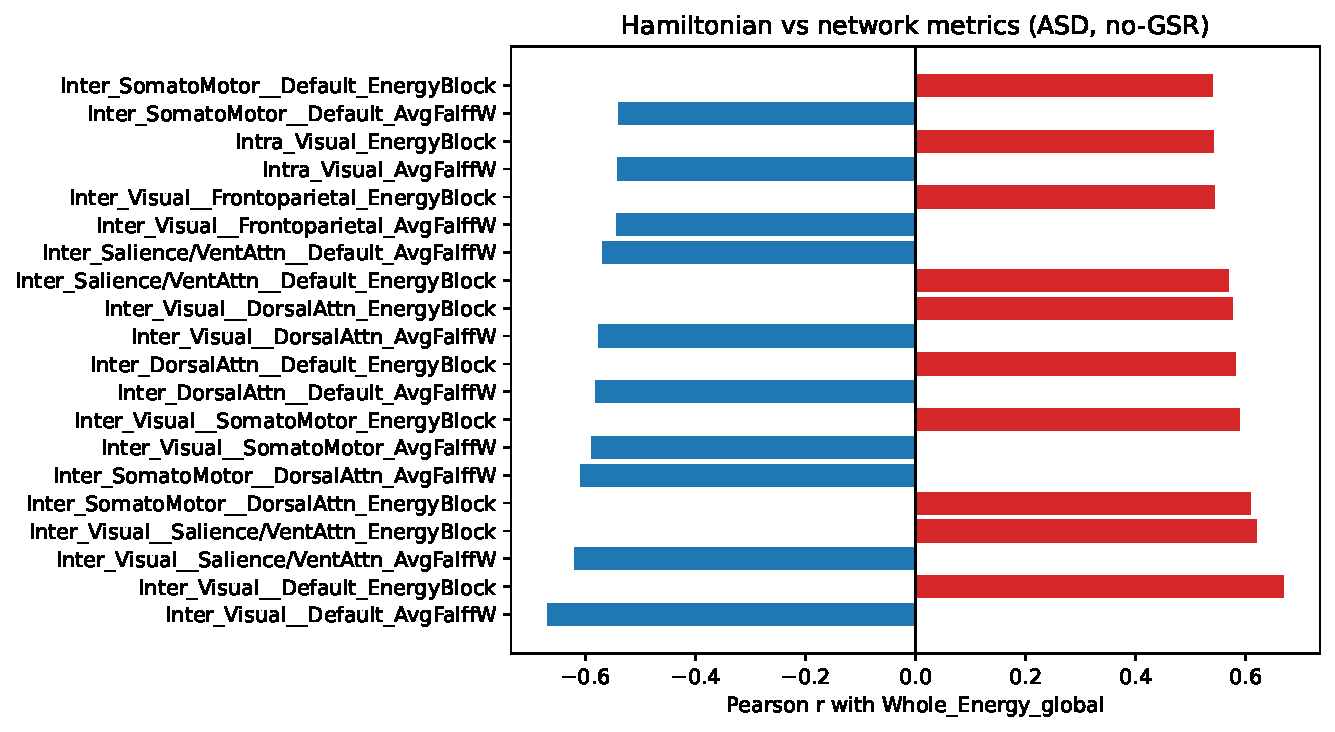
\includegraphics[width=0.85\linewidth]{Images/Hamiltonian_correlates_ASD_noGSR.pdf}
 \caption{Top 20 network metrics most strongly correlated with whole-brain coevolutionary energy
 ($H$) within the ASD group (no-GSR pipeline). Red bars indicate positive correlations (EnergyBlock
 features, which are negatively signed relatives of AvgFalffW and share the same information);
 blue bars indicate negative correlations. Note that AvgWeight features (pure FC magnitude, no
 fALFF-weighting) are also present among the strongest correlates, confirming that the Hamiltonian
 captures information beyond average connectivity. The two blue bars at the lower end of the ranking
 correspond to global and local graph efficiency; the global Hamiltonian is most directly compared
 with global efficiency, and the local efficiency measure provides the corresponding local-scale
 comparison. Their negative correlation with $H$ within ASD (FDR $p = 0.006$) indicates that more
 coevolutionarily stable networks tend to be less efficiently integrated.}
 \label{fig:hamil_correlates}
\end{figure}

\paragraph*{Intra-network metrics.}
At the intra-network level, only Dorsal Attention network average connectivity (AvgWeight) showed
an uncorrected group difference (ASD: $0.274 \pm 0.118$; TD: $0.310 \pm 0.121$; $p = 0.039$),
with lower connectivity in ASD, but this did not survive FDR correction ($p_{\mathrm{FDR}} = 0.32$;
Fig~\ref{fig:noGSR_intra}). No other intra-network metrics reached uncorrected significance.

\begin{figure}[H]
 \centering
 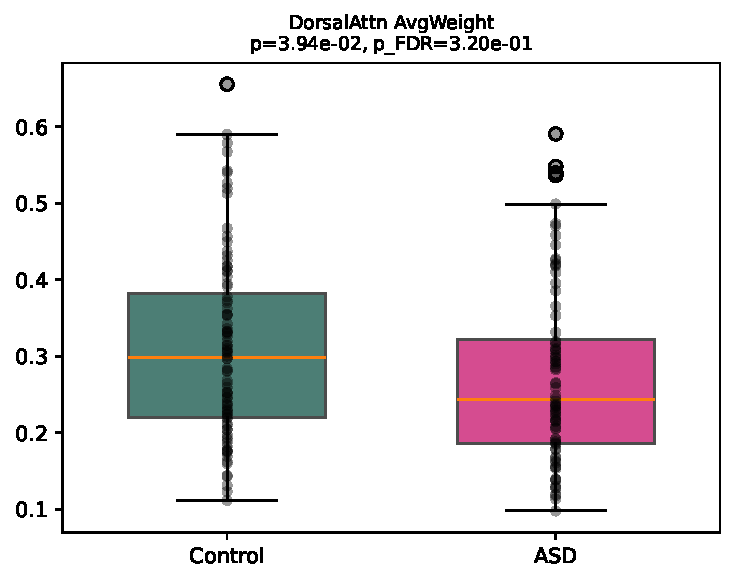
\includegraphics[width=0.55\linewidth]{Images/Intra_significant_noGSR.pdf}
 \caption{Intra-network metric showing the largest uncorrected group difference in the no-GSR
 analysis: Dorsal Attention network average connectivity ($p = 0.039$, $p_{\mathrm{FDR}} = 0.32$).
 This did not survive FDR correction.}
 \label{fig:noGSR_intra}
\end{figure}

\paragraph*{Inter-network metrics.}
No inter-network metrics reached significance after FDR correction in the no-GSR analysis (all
$p_{\mathrm{FDR}} > 0.35$). Several network pairs involving the dorsal attention and somatomotor
networks showed nominally significant trends in average connectivity (SomatoMotor--DorsalAttn:
$p = 0.050$; DorsalAttn--Limbic: $p = 0.058$; DorsalAttn--Default: $p = 0.059$;
Fig~\ref{fig:noGSR_inter}), consistent with the general pattern of lower connectivity in ASD
observed in the GSR analysis.

\begin{figure}[H]
 \centering
 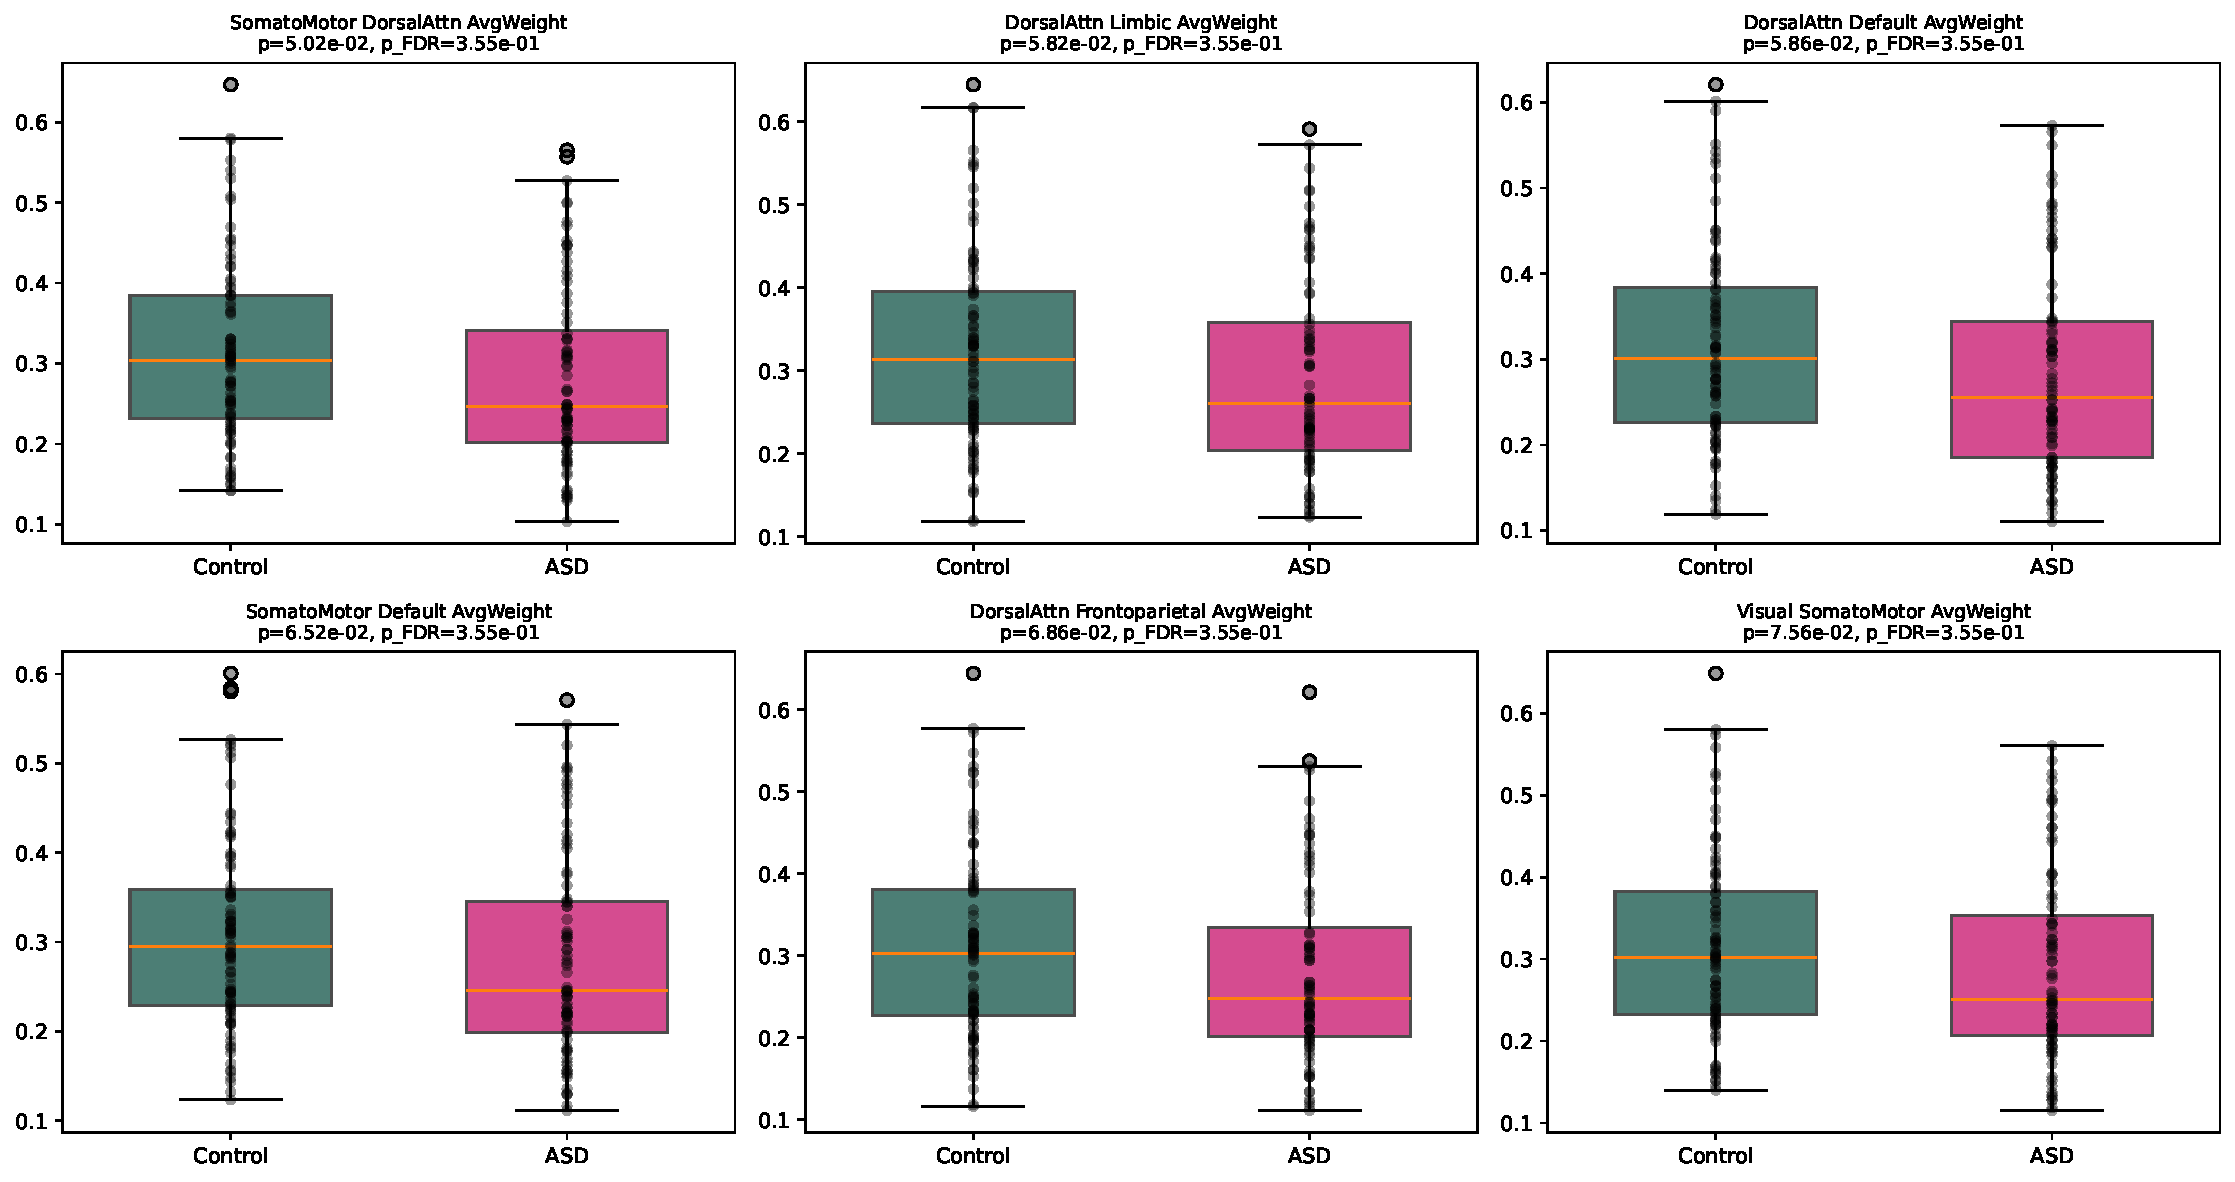
\includegraphics[width=0.95\linewidth]{Images/Inter_significant_noGSR.pdf}
 \caption{Inter-network average connectivity metrics with the smallest $p$-values in the no-GSR
 sensitivity analysis. None survived FDR correction (all $p_{\mathrm{FDR}} > 0.35$). Effects are
 generally weaker and fewer than in the GSR-based analysis.}
 \label{fig:noGSR_inter}
\end{figure}

\paragraph*{Behavioral correlations under CompCor preprocessing.}
Behavioral correlations were also computed under the no-GSR (CompCor) pipeline, providing a direct
comparison with the primary GSR results. Using
the same procedure (Pearson and Spearman $r$, FDR correction across 460 tests: 92 features
$\times$ 5 clinical scores with sufficient data), no feature--clinical score association survived
FDR correction ($q < 0.05$). At the nominally significant threshold ($p < 0.05$), 31 pairs were
detected across all five scores---again close to the chance expectation. The strongest associations
involved inter-network SomatoMotor--Default fALFF-aligned connectivity with ADOS Total ($r = -0.34$,
$p = 0.008$; $n = 60$), intra-network Limbic energy with ADOS Communication ($r = -0.37$,
$p = 0.009$; $n = 50$), and inter-network DorsalAttn--Limbic fALFF-aligned connectivity with ADI-R
Social ($r = +0.45$, $p = 0.008$; $n = 33$). The Hamiltonian did not show a significant within-ASD
correlation with ADOS Total in the no-GSR pipeline ($r = +0.05$, $p = 0.71$), consistent with the
GSR result ($r = -0.10$, $p = 0.47$): in neither pipeline, after harmonization, is whole-brain
energy associated with symptom severity.

\paragraph*{Machine learning classification.}
Classification under the no-GSR pipeline was also at or near chance after harmonization. The best
held-out test accuracy was $0.59$ (Gaussian Naive Bayes), with cross-validated accuracies of
$0.46$--$0.57$ across the five classifiers (Table~\ref{tab:noGSR_ml}; Fig~\ref{fig:noGSR_ml}).
As in the GSR pipeline, this is consistent with the absence of FDR-significant univariate group
differences: neither preprocessing strategy yields features that reliably discriminate ASD from TD
after site harmonization.

\begin{table}[ht]
\centering
\caption{Classification performance in the no-GSR sensitivity analysis (CompCor preprocessing) after
ComBat harmonization. All models performed at or near chance (cross-validated accuracy
$0.46$--$0.57$; held-out test accuracy $\leq 0.59$), consistent with the absence of FDR-significant
univariate group differences.}
\label{tab:noGSR_ml}
\small
\begin{tabular}{lccccc}
\toprule
Model & CV Acc & Test Acc & Test Bal Acc & Test F1 & Test AUC \\
\midrule
Gaussian Naive Bayes  & 0.567 & 0.588 & 0.594 & 0.611 & 0.531 \\
SVM (RBF)             & 0.530 & 0.500 & 0.503 & 0.514 & 0.554 \\
Logistic Regression   & 0.552 & 0.529 & 0.531 & 0.529 & 0.587 \\
KNN                   & 0.500 & 0.471 & 0.476 & 0.500 & 0.521 \\
XGBoost               & 0.455 & 0.559 & 0.559 & 0.545 & 0.556 \\
\bottomrule
\end{tabular}
\end{table}

\begin{figure}[H]
  \centering
  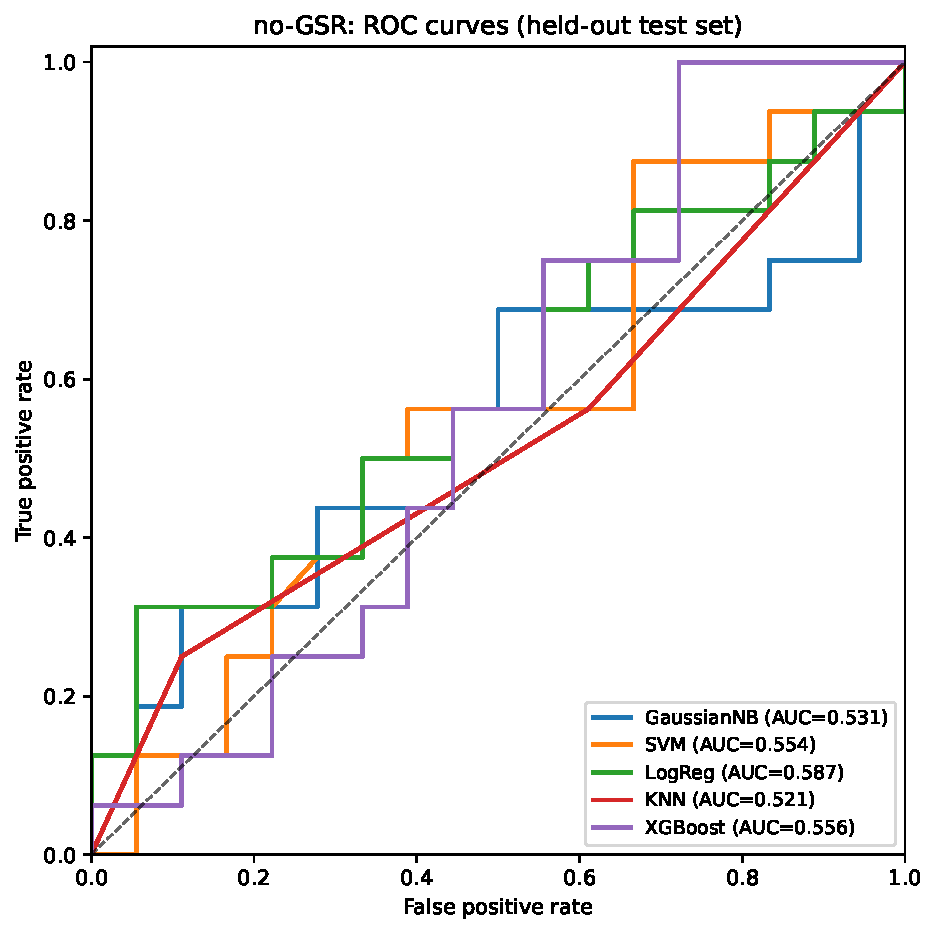
\includegraphics[width=0.6\linewidth]{Images/no-GSR_roc.pdf}
  \caption{ROC curves for ASD versus TD classification in the no-GSR sensitivity analysis (CompCor
  preprocessing, harmonized features). Curves lie near the chance diagonal; the best held-out test
  accuracy was $0.59$ (Gaussian Naive Bayes), again indicating near-chance discrimination, as in the
  GSR pipeline (Fig~\ref{fig:ml_confusion_roc}).}
  \label{fig:noGSR_ml}
\end{figure}

\paragraph*{Summary of the sensitivity analysis.}
Table~\ref{tab:GSR_comparison} provides a side-by-side comparison of key results across the two
preprocessing pipelines after harmonization, together with the effect of harmonization itself. The
two pipelines agree on the central outcome: after correct harmonization and FDR correction, no
whole-brain, intra-network, or inter-network feature differs significantly between groups under
either GSR or CompCor. The strongest nominal whole-brain trend differs by pipeline (more negative
energy under GSR, $p = 0.048$; slightly higher bipolarity under CompCor, $p = 0.026$), but neither
survives correction, and bipolarity does not differ at all under GSR. The within-ASD association
between $H$ and graph efficiency is the one effect that reaches FDR significance, and only in the
no-GSR pipeline. Classification on the harmonized features was at or near chance in both pipelines
(Tables~\ref{tab:ml_summary_full} and~\ref{tab:noGSR_ml}). These patterns are discussed further below, including the decisive
effect of harmonization itself.

\begin{table}[ht]
\centering
\caption{Comparison of key results across pipelines after correct site harmonization, and the
effect of harmonization itself. All group comparisons are FDR-corrected within their feature family.
``Pre-harm.'' denotes the earlier analysis in which ComBat had failed silently and raw features were
used.}
\label{tab:GSR_comparison}
\small
\begin{tabular}{lcc}
\toprule
\textbf{Finding} & \textbf{GSR (harmonized)} & \textbf{No-GSR / CompCor (harmonized)} \\
\midrule
Sample size (ASD / TD) & 78 / 86 & 78 / 87 \\
\midrule
\multicolumn{3}{l}{\textit{Effect of harmonization on whole-brain energy (GSR)}} \\
\quad Pre-harmonization & \multicolumn{2}{c}{$p_{\mathrm{FDR}} = 0.002$ (apparently significant)} \\
\quad Post-harmonization & \multicolumn{2}{c}{uncorrected $p = 0.048$, $p_{\mathrm{FDR}} = 0.19$ (n.s.)} \\
\midrule
\multicolumn{3}{l}{\textit{Whole-brain metrics (harmonized)}} \\
\quad Energy global & $p = 0.048$, $p_{\mathrm{FDR}} = 0.19$ (n.s.) & $p = 0.305$ (n.s.) \\
\quad Prop imbalanced same & $p = 0.047$, $p_{\mathrm{FDR}} = 0.19$ (n.s.) & $p = 0.109$ (n.s.) \\
\quad Bipolarity & $p = 0.53$ (n.s.) & $p = 0.026$, $p_{\mathrm{FDR}} = 0.21$ (n.s.) \\
\quad Graph efficiency (group diff.) & $p > 0.99$ (n.s.) & $p = 0.25$ (n.s.) \\
\midrule
\multicolumn{3}{l}{\textit{$H$--graph efficiency correlation (within ASD)}} \\
\quad Global efficiency & $r = -0.20$, $p = 0.075$ (n.s.) & $r = -0.33$, $p_{\mathrm{FDR}} = 0.005$ (sig.) \\
\midrule
\multicolumn{3}{l}{\textit{Intra-/Inter-network metrics}} \\
\quad FDR-significant effects & None & None \\
\midrule
\multicolumn{3}{l}{\textit{$H$--ADOS Total within-ASD correlation}} \\
\quad ADOS Total & $r = -0.10$, $p = 0.47$ (n.s.) & $r = +0.05$, $p = 0.71$ (n.s.) \\
\midrule
\multicolumn{3}{l}{\textit{Behavioral correlations / PLSC}} \\
\quad Any FDR-significant pair & 0 (of 460) & 0 (of 460) \\
\quad PLSC LV1 (ADOS block) & perm $p = 0.73$ (n.s.) & perm $p = 0.26$ (n.s.) \\
\midrule
\multicolumn{3}{l}{\textit{Classification (best held-out test accuracy; harmonized)}} \\
\quad Best model / accuracy & SVM / XGBoost, $0.65$ (CV $\approx 0.59$) & GaussianNB, $0.59$ (CV $\approx 0.57$) \\
\quad Interpretation & \multicolumn{2}{c}{near chance in both pipelines} \\
\bottomrule
\end{tabular}
\end{table}

\section*{Discussion}

In this study we used a coevolutionary balance framework to characterize how resting-state
functional networks are organized in adult males with autism spectrum disorder. By combining
binarized regional activity (fractional amplitude of low-frequency fluctuations, fALFF) with
signed functional connectivity (FC) in a single Hamiltonian, we derived multi-scale energy-based
descriptors that jointly capture nodal states and link signs \cite{Heider:1946ac,cartwright1956,
Kargaran:2021he,GhanbarzadehNoudehi2022}. We examined these descriptors at whole-brain, intra-network,
and inter-network levels, evaluated them against topology-preserving null models, related them to
clinical measures, assessed their relationship with global and local graph efficiency, and tested
their utility in supervised classification. Critically, ComBat harmonization was applied to mitigate
multi-site batch effects \cite{Fortin2017,Johnson2007}, and all analyses were repeated with and
without GSR to assess sensitivity of signed connectivity measures to this preprocessing choice.
The no-GSR pipeline corresponds precisely to a CompCor-based denoising approach. Overall, after
correct site harmonization the framework did not reveal statistically robust ASD--TD differences:
the apparent whole-brain effects seen before harmonization did not survive it, and no feature in
either pipeline survived FDR correction. We discuss what this implies for the framework and for
signed-network analyses of multi-site data below.

\paragraph*{Whole-brain coevolutionary characterization of ASD.}
At the whole-brain level, autistic participants showed nominally more negative coevolutionary energy
than typically developing controls under the GSR pipeline (ASD: $-139.7 \pm 78.7$; TD:
$-118.8 \pm 76.2$; uncorrected $p = 0.048$), in the direction of energetically more favorable
configurations in which highly active regions are positively coupled and less active regions are
negatively coupled. However, this difference did not survive FDR correction across the eight
whole-brain features ($p_{\mathrm{FDR}} = 0.19$). The motif descriptors derived from the same
Hamiltonian followed the same direction---a nominally higher proportion of agreement links and lower
proportion of imbalanced-same links in ASD---but these effects were also non-significant after
correction ($p_{\mathrm{FDR}} = 0.19$). Bipolarity did not differ between groups under GSR
($p = 0.53$); it showed only a nominal, non-significant trend in the no-GSR sensitivity analysis
($p = 0.026$, $p_{\mathrm{FDR}} = 0.21$; see below). We emphasize that an earlier, un-harmonized
version of this analysis produced an apparently strong and FDR-significant energy effect; that effect
did not survive correct site harmonization (see ``Effect of site harmonization''), indicating that
it was substantially driven by between-site variance rather than by ASD-related biology. Taken
together, the harmonized whole-brain results provide, at most, weak and uncorrected directional
hints of more favorable coevolutionary configurations in ASD, and no statistically robust group
difference in global coevolutionary organization.

When projected onto canonical Yeo systems \cite{Yeo2011}, intra-network coevolutionary energy did
not differ between groups, reaching neither FDR-corrected nor nominal significance after
harmonization. The inter-network analyses likewise revealed no FDR-significant effects; the strongest
trend was higher SomatoMotor--Frontoparietal connectivity in ASD ($p_{\mathrm{FDR}} = 0.069$). These
patterns are exploratory and indicate that, in the harmonized data, there is no robust localization
of coevolutionary alterations to individual canonical networks.

\paragraph*{Brain--behavior relationships.}
After harmonization, we found no robust relationship between any coevolutionary or connectivity
metric and symptom severity. In particular, the whole-brain Hamiltonian was uncorrelated with ADOS
Total within ASD in both pipelines (GSR: $r = -0.10$, $p = 0.47$; no-GSR: $r = +0.05$, $p = 0.71$).
A negative $H$--ADOS correlation ($r = -0.26$, $p = 0.017$) that was present in the pre-harmonization
GSR analysis did not survive harmonization, and no behavioral association in either pipeline survived
FDR correction. We therefore do not interpret any directional brain--behavior pattern as established.
Conceptually, it remains true that within-network and inter-network connectivity enter the
Hamiltonian differently depending on the sign configuration of the relevant nodes, so that
within-group correlations between $H$ and mean connectivity (e.g.\ $r \approx -0.31$ within ASD in
the no-GSR pipeline) reflect the signed alignment of links with nodal states rather than overall
connectivity magnitude. This is a property of the framework rather than a group-level or
clinical finding.

\paragraph*{Within-group structure of the framework.}
Although no group difference survived correction, the coevolutionary energy behaved coherently as a
description of signed network organization within each group. In the no-GSR pipeline, more negative
$H$ within ASD was significantly associated with lower global and local graph efficiency
($r = -0.33$, FDR $p = 0.005$) and with lower mean connectivity across several network pairs
($r \approx -0.31$, FDR $p \approx 0.009$), indicating that---within autistic individuals---greater
coevolutionary stability co-occurs with reduced network integration and lower overall connectivity.
This relationship was weaker and non-significant in TD ($r = -0.17$) and only a non-significant trend
within ASD in the GSR pipeline ($r = -0.20$), so it is best regarded as an exploratory,
pipeline-dependent observation rather than a robust ASD-specific mechanism. These are within-group
correlations describing how the Hamiltonian relates to standard graph metrics; they do not establish
any ASD--TD difference.

\paragraph*{Multivariate behavioral analysis.}
The multivariate analyses reinforced the univariate null. Cross-validated PLS regression produced
negative $R^2$ for all clinical scores, and an exploratory PLS correlation (PLSC) analysis found no
significant latent variable linking network features to behavior (first latent variable: permutation
$p = 0.73$ with GSR, $p = 0.26$ without GSR). With 92 features and $n = 29$--59 per score, these
analyses are underpowered, and the null results reflect an absence of detectable structure in this
sample rather than evidence against any relationship.

\paragraph*{Effect of site harmonization.}
The most consequential methodological observation concerns harmonization itself. In an earlier
version of this analysis, ComBat failed silently on a single-participant site and the pipeline
reverted to un-harmonized features; under those conditions the whole-brain energy difference appeared
strong and FDR-significant ($p_{\mathrm{FDR}} \approx 0.002$) and supervised classification appeared
well above chance. Once harmonization was correctly applied---after excluding the single- and
two-participant sites---the same whole-brain energy contrast fell to an uncorrected $p = 0.048$
($p_{\mathrm{FDR}} = 0.19$), and no feature in either pipeline survived correction. Because diagnostic
group was included as a protected covariate, ComBat could remove only site-related variance, not
genuine group structure; the collapse of the effect therefore indicates that the apparent ASD--TD
difference was largely attributable to between-site variance rather than to autism-related biology.
This is consistent with the well-documented magnitude of site effects in ABIDE and with the
sensitivity of signed-network measures to preprocessing. We report this transparently as a cautionary
result: in multi-site signed-network analyses, harmonization is not a cosmetic step but can determine
whether a group effect is present at all.

\paragraph*{Preprocessing and classification.}
The two pipelines agreed in showing no FDR-significant group differences, although the strongest
nominal whole-brain trend differed (energy under GSR; bipolarity under CompCor), reflecting the known
effect of GSR on the sign structure of functional connectivity \cite{Murphy2009,Fox2009,Chang2009}:
by shifting the distribution of FC toward zero and introducing anticorrelations, GSR alters the
signed network structure that the coevolutionary Hamiltonian encodes. Supervised classification on
the harmonized features was at or near chance in both pipelines (best held-out test accuracy
$\approx 0.65$ with GSR and $0.59$ without GSR, on cross-validated accuracies of $\approx 0.57$--$0.59$),
confirming that the harmonized coevolutionary and connectivity features do not carry a reliable
ASD--TD diagnostic signal. The substantially higher accuracy obtained before harmonization
($\approx 0.78$) was therefore another manifestation of the uncorrected site structure rather than a
genuine diagnostic signal.

\paragraph*{Interpretation of the framework.}
Taken together, these results do not support coevolutionary energy as a site-robust biomarker of ASD
in this adult ABIDE sample. They do, however, show that the framework is internally coherent and
interpretable: it integrates nodal activity and signed connectivity into a single energetic
description, relates sensibly to established graph metrics within groups, and makes the influence of
preprocessing and site effects explicit and measurable. Classical graph-theoretic analyses typically
treat node-wise and edge-wise measures separately; the present Hamiltonian explicitly encodes how
nodal states and link signs co-align. We therefore present coevolutionary balance as a
methodologically sound descriptive tool whose careful application here yields a rigorous null for
ASD--TD group differences, rather than as evidence that autistic brains occupy a distinct
coevolutionary minimum.

\paragraph*{Limitations and future directions.}
The present analyses were restricted to adult males from ABIDE I and therefore do not generalize
to females, younger individuals, or autistic individuals with intellectual disability. Despite
ComBat harmonization, residual site-related variability cannot be fully excluded, and the inherent
heterogeneity of ABIDE in scanner hardware and behavioral protocols remains a limitation. As
demonstrated by our sensitivity analysis, GSR substantially affects the sign structure of functional
connectivity and consequently the coevolutionary energy measures derived from it; the primary
GSR-based results should be interpreted with this caveat in mind, and the no-GSR/CompCor results
provide an important complementary perspective. The binarization of fALFF into high versus low
values using a subject-specific median threshold simplifies the underlying continuous distribution,
and the use of static functional connectivity collapses potentially important temporal dynamics.
The choice of the CC200 parcellation and Pearson correlation--based signed connectivity may also
influence the derived energy metrics; future work should examine robustness across parcellations,
preprocessing strategies, and dynamic connectivity estimators. Because the no-GSR and GSR pipelines
applied identical outlier removal to their respective, pipeline-specific energy distributions, their
final samples differ slightly (78/86 versus 78/87); although both derive from the same initial
cohort and quality control, restricting both pipelines to the identical participant set would provide
an even more direct comparison and is a worthwhile refinement for future analyses. Our auxiliary
integration measure, graph efficiency, was computed on absolute-valued weights and is therefore
sign-agnostic; weight-conserving, sign-aware descriptors such as signed modularity
\cite{RubinovSporns2011} would provide a more faithful topological characterization of the positive
and negative connection systems and are a natural complement to the coevolutionary energy in future
work. The cross-sectional design limits
inferences about developmental trajectories or causal mechanisms. Behavioral correlations and PLS
analyses were underpowered due to the limited number of ASD participants with complete clinical
data ($n = 29$--59 per score), and none survived FDR correction; larger datasets are essential
for brain--behavior analyses. Finally, while machine-learning results under the GSR pipeline are
encouraging, validation in larger independent datasets is essential.

Future work should address these limitations through longitudinal and developmental designs,
time-resolved extensions relating dynamic Hamiltonian changes to moment-to-moment network
fluctuations, and integration of coevolutionary descriptors with genetic, cognitive, and behavioral
data. Extending the framework to cellular-resolution calcium imaging data would allow direct
testing of the excitation--inhibition balance interpretation of coevolutionary stability. These
directions highlight that energy-based descriptions are a complementary tool that can provide a
physically grounded perspective on how large-scale brain networks are organized in neurodevelopmental
conditions such as autism.

\section*{Methods}

\subsection*{Participants and Dataset}
We obtained resting-state fMRI data from the Autism Brain Imaging Data Exchange I (ABIDE I)
repository \cite{DiMartino:2014abide}. The ABIDE I dataset used in this study was accessed via the NITRC-IR 
data-sharing platform on October 9, 2025. A priori power analysis in G*Power (two-tailed, $\alpha=0.05$,
$1-\beta=0.80$, $d=0.50$) showed that there needed to be at least 64 individuals in each group
\cite{Faul2009}. We randomly selected 100 males with a clinical diagnosis of ASD and 100 age- and
IQ-matched TD men who were all right-handed, between 18 and 30 years of age, and had a full-scale
IQ greater than 80. This was done to allow for the removal of outliers and site-specific variability.
Data were drawn from 14 contributing sites. Certified clinicians at each site used the Autism
Diagnostic Observation Schedule (ADOS) and the Autism Diagnostic Interview--Revised (ADI-R) to
confirm ASD diagnosis according to DSM-5 criteria \cite{APA:2022ds}.

\begin{table}[H]
\centering
\caption{Demographic and sampling characteristics of the study cohort.}
\label{tab:demographics}
\setlength{\tabcolsep}{3pt}
\small
\resizebox{\columnwidth}{!}{%
\begin{tabular}{p{0.38\columnwidth}p{0.27\columnwidth}p{0.27\columnwidth}}
\toprule
\textbf{Characteristic} & \textbf{ASD} & \textbf{TD} \\
\midrule
Initially selected from ABIDE I, $n$ & 100 & 100 \\
Analyzed sample after QC, harmonization, and outlier removal (GSR), $n$ & 78 & 86 \\
Sex (male / female), $n$ & all male & all male \\
Age range (years) & 18--30 & 18--30 \\
Handedness & right & right \\
Full-scale IQ (FSIQ) inclusion & $>$ 80 & $>$ 80 \\
Diagnostic status & DSM ASD, ADOS/ADI-R confirmed & Typically developing (TD), no ASD diagnosis \\
Data source / preprocessing & ABIDE I, CPAC pipeline, CC200 atlas (200 ROIs) & ABIDE I, CPAC pipeline, CC200 atlas (200 ROIs) \\
Contributing sites (after excluding single/two-subject sites) & 11 & 11 \\
No-GSR (CompCor) analyzed sample (ASD / TD) & 78 / 87 & 78 / 87 \\
\bottomrule
\end{tabular}%
}
\begin{flushleft}
\footnotesize
All participants were right-handed adult males (18--30 years) with full-scale IQ greater than 80,
randomly selected from the ABIDE I repository and matched on age and IQ across groups. Both pipelines
were applied to the same initially selected cohort (100 ASD, 100 TD) and used identical inclusion and
motion-based quality-control criteria; the two pipelines differ only in the nuisance-regression step
(GSR versus CompCor). Prior to ComBat harmonization, two acquisition sites contributing only one
(CMU) or two (UCLA\_1) participants were excluded, as a single-participant batch cannot be
harmonized; this left 11 sites. After ComBat harmonization and Tukey IQR-based outlier removal on
whole-brain coevolutionary energy, the GSR analysis sample comprised 78 ASD and 86 TD participants,
and the no-GSR (CompCor) sample comprised 78 ASD and 87 TD participants. The small difference in
final sample size between pipelines reflects pipeline-specific outlier removal applied to each
pipeline's own energy distribution.
\end{flushleft}
\end{table}

Participants were excluded if they had neurological comorbidities (such as epilepsy or traumatic
brain injury), a mean framewise displacement greater than 0.5 mm or more than 20\% of volumes
exceeding this criterion \cite{Faul2009}, or incomplete demographic or behavioral data. After
quality control and the exclusion of single/two-participant sites prior to harmonization, 78 ASD
and 86 TD participants remained in the GSR analysis (78 ASD and 87 TD in the no-GSR analysis). The
two groups were matched for age
(ASD: $24.3\pm3.1$ y; TD: $24.1\pm3.2$ y; $p=0.72$) and IQ (ASD: $105.2\pm9.8$; TD:
$106.4\pm10.1$; $p=0.65$). All models included the scanner site as a nuisance covariate where
applicable.

\subsection*{Imaging Preprocessing and fALFF Computation}
We used CPAC v1.0 \cite{Craddock:2013cpac} to preprocess all functional images. This included
correcting slice timing with sinc interpolation, correcting rigid body motion with six parameters
and derivatives (a total of 24 regressors), coregistering each subject's T1 image, normalizing
to MNI152 (3 mm isotropic), and smoothing the images spatially with a 6 mm FWHM. In the primary
analysis pipeline, nuisance regression removed linear and quadratic trends, global signal, white
matter, and CSF signals, as well as motion regressors. We used a zero-phase Butterworth band-pass
filter on the residual time series (0.01--0.1 Hz). We computed fALFF voxel-wise using the Fast
Fourier Transform: ALFF was the average square-rooted power in the frequency range of 0.01 to
0.08 Hz, divided by the total power in the frequency range of 0 to 0.25 Hz
\cite{Zang:2007al,Zou:2008fa}. The mean fALFF was extracted for each ROI in the CC200 atlas
\cite{Craddock:2012atlas}.

Because global signal regression (GSR) has been shown to introduce artifactual negative correlations
that may affect the sign structure of functional connectivity \cite{Murphy2009,Fox2009,Chang2009},
and since signed link polarity is a key parameter in the coevolutionary balance framework, we
additionally repeated all analyses using a preprocessing pipeline in which GSR was omitted. In
this alternative pipeline, nuisance regression included only white matter and CSF signals
(CompCor-based denoising; \cite{Behzadi2007}), linear and quadratic trends, and motion regressors,
but did not include global signal removal. All subsequent steps (fALFF computation, parcellation,
network construction, ComBat harmonization, and statistical analyses) were identical to the primary
pipeline. Results from both pipelines are reported: the GSR-based analysis as the primary analysis
and the no-GSR/CompCor analysis as a sensitivity check.

\paragraph*{Binarization of fALFF values.}
To obtain the binary node states required by the coevolutionary Hamiltonian, each participant's
regional fALFF values were thresholded at the subject-specific median. Regions with fALFF values
at or above the median were assigned $s_i = +1$ (high intrinsic activity), and regions below the
median were assigned $s_i = -1$ (low intrinsic activity). This median split ensures scale-free
comparability across subjects and prevents bias from global fALFF amplitude differences. All
coevolutionary energy and motif analyses used these binarized activity states.

\subsection*{Parcellation and Time Series Harmonization}
We used the CC200 atlas in MNI space to define 200 ROIs. To ensure consistency across all sites,
all subjects' time courses were truncated to the smallest number of volumes found in any scan
following preprocessing. This ensured that correlation analyses had the same number of samples.

\subsection*{Network Construction}
We built an undirected weighted graph $G=(V,E)$ with $|V|=200$ for each subject. The edge weight
$w_{ij}$ was computed as the Pearson correlation between the preprocessed time series of ROIs $i$
and $j$, followed by Fisher $z$-transformation to improve normality. No additional thresholding was
applied; the complete matrix was retained for analysis. Using the full weighted matrix preserves
the graded information in both positive and negative connections and allows the Hamiltonian to
capture contributions from all signed edges \cite{Smith:2013fc,Fornito2016}.

\subsection*{ComBat Harmonization}
To address multi-site batch effects inherent in pooled neuroimaging datasets, we applied ComBat
harmonization \cite{Johnson2007,Fortin2017} to the derived network features. ComBat uses an
empirical Bayes framework to estimate site-specific location (mean) and scale (variance) parameters
and removes these batch effects while preserving biological variability of interest.

Specifically, for each network feature $y_{ij}$ (where $i$ indexes subjects and $j$ indexes
features), we modeled:
\[
y_{ij} = \alpha_j + X_i \beta_j + \gamma_{i(s)j} + \delta_{i(s)j} \epsilon_{ij}
\]
where $\alpha_j$ is the overall mean for feature $j$, $X_i$ is a design matrix of biological
covariates of interest (diagnostic group), $\beta_j$ is the coefficient vector, $\gamma_{i(s)j}$
is the additive site effect for subject $i$ at site $s$, $\delta_{i(s)j}$ is the multiplicative
site effect, and $\epsilon_{ij}$ is the residual error. ComBat estimates these parameters using
empirical Bayes shrinkage and produces harmonized data by removing the site effects. We applied
ComBat to the full feature matrix after initial quality control, using diagnostic group (and IQ) as
the biological covariates to preserve. All subsequent statistical analyses and machine learning were
performed on the ComBat-harmonized features.

Because ComBat estimates a location and scale parameter per site, sites contributing only one or two
participants cannot be reliably harmonized; a single-participant site in particular makes the
empirical Bayes variance estimate undefined and causes the harmonization to fail. We therefore
excluded the two smallest sites (CMU, with one participant, and UCLA\_1, with two) prior to
harmonization, leaving 11 sites. We additionally verified that the harmonized feature matrix
contained no missing values and that it differed from the raw feature matrix (confirming that the
harmonization was in fact applied), rather than allowing any silent fallback to un-harmonized data.
Both the GSR and no-GSR pipelines were harmonized identically under this procedure.

\subsection*{Coevolutionary Balance Theory}
We used a discrete coevolutionary balance formulation in which each brain region is assigned a
binary activity state, and functional interactions contribute according to their signed connectivity
weight \cite{Heider:1946ac,cartwright1956,Kargaran:2021he,GhanbarzadehNoudehi2022}. For each
participant, the nodal state $s_i \in \{-1,+1\}$ was derived by thresholding regional fALFF at
the subject-specific median. The signed functional connectivity weight $w_{ij}$ was obtained from
the Fisher-$z$-transformed correlation between regional BOLD time series.

The corresponding coevolutionary energy was defined as
\begin{equation}
H(G) = -\sum_{i<j} s_i \, w_{ij} \, s_j.
\label{eq:hamiltonian}
\end{equation}
This Hamiltonian reaches more negative values when regions with the same activity state are
positively connected and oppositely active regions are negatively connected, and increases when
these relationships are inconsistent. The four possible pairwise configurations of nodal states
and link signs, together with their energetic consequences, are illustrated in
Fig~\ref{fig:configuration}.

\begin{figure}[H]
 \centering
 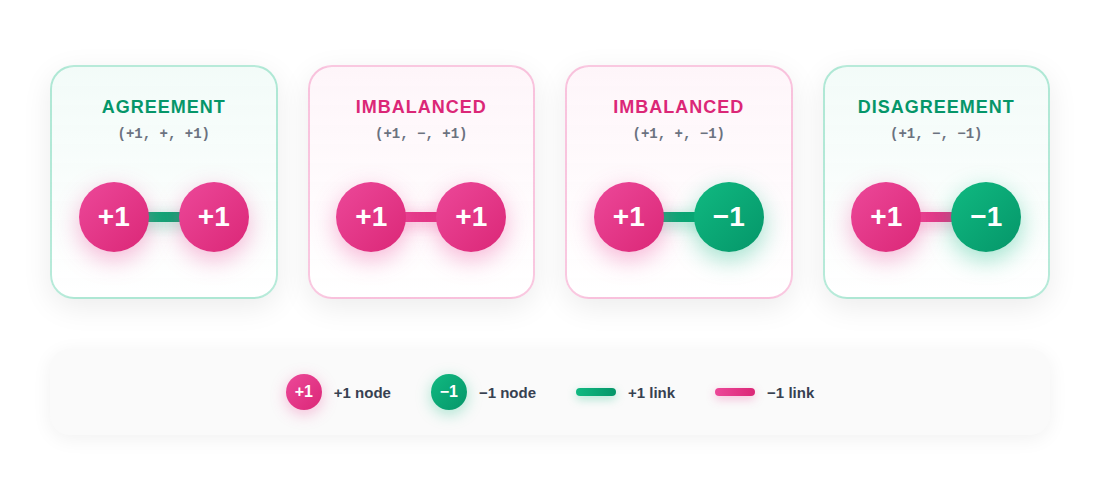
\includegraphics[width=0.8\linewidth]{Images/figure_configurations_v2.png}
 \caption{Pairwise configurations in the notion of coevolutionary equilibrium. The blue and orange
 circles show the states of the nodes ($+1$ and $-1$) representing high vs.\ low fALFF, while the
 green and red lines show the signs of the links ($+1$ and $-1$) representing positive vs.\ negative
 FC. Agreement configurations lower energy, while imbalanced pairs raise it.}
 \label{fig:configuration}
\end{figure}

\paragraph*{Signed motif proportions and bipolarity.}
Each edge $(i,j)$ was assigned to one of four motif classes according to the sign of its
connectivity weight and the product of the nodal states it links. Edges with $s_i s_j = +1$ and
$w_{ij} > 0$ (\emph{agreement}) and edges with $s_i s_j = -1$ and $w_{ij} < 0$ (\emph{disagreement})
are energetically favorable and lower $H$, whereas edges with $s_i s_j = +1$ and $w_{ij} < 0$
(\emph{imbalanced-same}) and edges with $s_i s_j = -1$ and $w_{ij} > 0$ (\emph{imbalanced-opposite})
are unfavorable and raise $H$. For every subject we recorded the proportion of edges in each class
relative to the total number of edges; the four proportions sum to one.

Bipolarity $\beta$ quantifies the extent to which the \emph{signed connectivity} of a network can be
partitioned into two internally cohesive, mutually antagonistic blocks, independently of the
fALFF-derived activity states. Let $S$ be the sign matrix with $S_{ij} = \operatorname{sign}(w_{ij})$
for $i \neq j$ and $S_{ii} = 0$, and let $D = \operatorname{diag}(d_i)$ with $d_i = \sum_{j} |S_{ij}|$
denote the corresponding degree matrix. From the signed graph Laplacian $L = D - S$ we computed the
eigenvector $v$ associated with the second-smallest eigenvalue (the spectral bipartitioning, or
Fiedler-type, vector) and assigned each node to one of two blocks according to $\sigma_i =
\operatorname{sign}(v_i)$. Bipolarity is then the fraction of edges whose sign is consistent with
this bipartition,
\begin{equation}
\beta = \frac{1}{|E|}\sum_{i<j}
\mathbf{1}\!\left[\operatorname{sign}(w_{ij})\,\sigma_i\,\sigma_j > 0\right],
\label{eq:bipolarity}
\end{equation}
where consistency means that positive edges fall \emph{within} a block ($\sigma_i = \sigma_j$) and
negative edges fall \emph{between} blocks ($\sigma_i \neq \sigma_j$). A value of $\beta = 1$
corresponds to a perfectly bipolar (exactly two-block balanced) network, whereas $\beta \approx 0.5$
indicates no preferred two-block organization. Bipolarity therefore characterizes global two-block
structure that is complementary to, and not determined by, the edge-wise motif proportions.

\subsection*{Graph efficiency computation}
Global and local graph efficiency were computed from the absolute-value weighted FC matrix for each
subject \cite{Latora2001,Fornito2016}. The edge-length matrix was defined as $d_{ij} = 1 /
|w_{ij}|$ for connected pairs (with $|w_{ij}| > 0$) and infinity otherwise. Global efficiency was
computed as the mean of the inverse shortest-path lengths across all pairs $i \neq j$:
\[
E_{\mathrm{global}} = \frac{1}{N(N-1)} \sum_{i \neq j} \frac{1}{d_{ij}^*}
\]
where $d_{ij}^*$ is the length of the shortest path between nodes $i$ and $j$ in the graph, and
$N = 200$ is the number of nodes. Shortest paths were computed using Dijkstra's algorithm as
implemented in SciPy. Local efficiency was computed as the global efficiency of the subgraph
induced by each node's immediate neighbors, averaged across nodes:
\[
E_{\mathrm{local}} = \frac{1}{N} \sum_i E_{\mathrm{global}}(G_i)
\]
where $G_i$ is the subgraph of neighbors of node $i$. Both metrics were included in the feature
matrix alongside the coevolutionary and connectivity measures, and were subjected to the same
ComBat harmonization, outlier removal, and statistical pipeline as all other features.

We note that, because graph efficiency is conventionally defined for positively weighted graphs,
it was computed here from the absolute value of the signed connectivity. This choice collapses the
distinction between positive and negative connections, which can carry different topological
information \cite{RubinovSporns2011}. Graph efficiency is therefore used here only as an auxiliary,
sign-agnostic descriptor of integration, and is not intended as a signed counterpart to the
coevolutionary energy. Weight-conserving measures that explicitly retain edge sign, such as signed
modularity \cite{RubinovSporns2011}, provide a complementary characterization of signed network
organization and are a natural target for future work (see Discussion).

\subsection*{Null-model construction}
To test whether empirical energies differed from chance expectations, we generated 1,000
topology-preserving null networks per subject. In each null replicate, nodal activity states
($s_i$) were randomly permuted across nodes, and edge signs were independently reassigned by
randomly permuting the signed weights across edges, while keeping the underlying adjacency structure
fixed. This degree-preserving randomization strategy follows the logic of the Maslov--Sneppen
rewiring framework \cite{Maslov2002}, adapted here for signed weighted networks. The procedure
destroys any systematic alignment between fALFF-derived nodal states and the sign structure of
functional connectivity while preserving the degree distribution, weight distribution, and density
of the original network \cite{Rubinov2010}. For each subject we computed the difference between
the empirical energy and the mean null energy.

\subsection*{Statistical Analysis}
All statistical group comparisons were conducted using an adaptive pipeline that selects the
appropriate statistical test based on the distributional properties of each individual metric.
Prior to any comparison, we assessed normality for each metric's distribution in the ASD and TD
groups separately using the Shapiro--Wilk test, and assessed homogeneity of variances using
Levene's test \cite{levene1960}. If both groups passed the Shapiro--Wilk criterion ($p > 0.05$)
and Levene's test also indicated equal variances, a standard independent-samples $t$-test was
applied. If both groups were normal but Levene's test indicated unequal variances, Welch's $t$-test
was applied. If either group failed the Shapiro--Wilk normality test, Mann--Whitney $U$ was used.
This decision was made independently for each feature before inspecting group differences, ensuring
that test selection was not influenced by the resulting $p$-values.

In practice, 87\% of all 92 features (80 out of 92) failed normality in at least one group: all 8
whole-brain features and all 21 intra-network features were non-normal in both groups, and 51 of
63 inter-network features were non-normal in at least one group. Mann--Whitney $U$ was therefore
applied to 80 features, the standard $t$-test to 10 features, and Welch's $t$-test to 2 features.
Full Shapiro--Wilk and Levene test statistics for every feature are provided in Supplementary
Table~\ref{tab:supp_normality}, which allows independent verification of each test decision and
confirms that the predominance of non-parametric testing reflects the empirical data, not a
post-hoc choice. All tests were two-tailed with $\alpha = 0.05$. Cohen's $d$ was used to report
parametric effect sizes. Where applicable, $p$-values were subsequently adjusted for multiple
comparisons using the Benjamini--Hochberg FDR correction applied separately within each feature
family (Whole, Intra, Inter).

\paragraph*{Unified outlier removal.}
Outlier removal was performed once using a single criterion based on whole-brain coevolutionary
energy. For each group separately (ASD and TD), subjects whose whole-brain energy fell outside
1.5 times the interquartile range (Tukey's IQR rule) were excluded. The same participant set was
used for all subsequent analyses.

\subsection*{Connectivity, fALFF-weighted connectivity, and block-wise energy}

To relate coevolutionary energy to canonical large-scale systems, we projected the CC200
parcellation onto the seven-network cortical atlas of Yeo et al.\ \cite{Yeo2011}. For each CC200
ROI we computed the Dice overlap with each Yeo7 network and assigned the ROI to the network with
maximal Dice coefficient.

For each subject we constructed a $7\times7$ block representation of connectivity and energy. For
each ordered pair of networks $(u,v)$ we computed three block-wise quantities: the mean functional
connectivity ($\mathrm{AvgWeight}_{uv}$), the mean fALFF-weighted connectivity
($\mathrm{AvgFalffW}_{uv}$), and the block-wise coevolutionary energy contribution ($E_{uv}$). All
connectivity and block-wise energy metrics were subjected to ComBat harmonization prior to
statistical analysis.

\subsection*{Correlation Analysis with Behavioral Measures}

To assess the clinical relevance of the energy-based network measures, we conducted a comprehensive
correlation analysis between all 92 ComBat-harmonized network features and five clinical scores
from the ADI-R and ADOS instruments. The clinical measures included ADI-R Social Total A, ADI-R
Verbal Total BV, ADI-R Onset Total D, ADOS Total, and ADOS Communication (the subscales with
sufficient data). ABIDE sentinel values ($-9999$) were treated as missing
data. Correlations were computed only for ASD participants with valid clinical data on a per-score
basis, resulting in sample sizes ranging from $n = 29$ (ADI-R Onset Total D) to $n = 59$
(ADOS Total).

For each of the 460 feature--clinical score combinations (92 features $\times$ 5 scores), we
computed both Pearson's $r$ and Spearman's $\rho$, along with exact two-tailed $p$-values. To
control for multiple comparisons, we applied Benjamini--Hochberg FDR correction separately to
the Pearson and Spearman $p$-values across all 460 tests. We additionally conducted a Partial
Least Squares (PLS) multivariate analysis for each clinical score, using all 90 standardized
features as predictors, with up to three components and stratified five-fold cross-validation
using $R^2$ as scoring metric. PLS regression was estimated with the NIPALS algorithm as
implemented in \texttt{scikit-learn} (\texttt{PLSRegression}), following the PLS framework for
neuroimaging reviewed by Krishnan et al.\ \cite{Krishnan2011}. We used the regression form of PLS
(PLSR) because each clinical score was modelled as a continuous outcome and predictive performance
was the quantity of interest; the closely related Partial Least Squares Correlation (PLSC, or
behavioural PLS) variant, which performs a singular value decomposition of the brain--behaviour
cross-correlation matrix and is evaluated by permutation testing rather than out-of-sample
prediction \cite{Krishnan2011}, offers a complementary, purely descriptive view of the same
covariance structure. The PLS results are reported as a multivariate complement to the univariate
tests.

For the no-GSR (CompCor) pipeline, behavioral correlations were computed analogously using the
92-feature set (including graph efficiency), testing 460 feature--score combinations (92 features
$\times$ 5 clinical scores with $n \geq 20$).

\subsection*{Machine learning classification of ASD versus TD}

To examine whether the derived graph-based features carry discriminative information about
diagnostic status, we performed supervised classification analyses on the adult male ABIDE I
subsample with complete feature data. Feature selection was carried out using a Random Forest
classifier fitted on the training set only. We computed the mean decrease in impurity importance
for each feature, ranked features by importance, and retained the top 25\% (23 features) as the
final input set. All 90 features (or 92 including efficiency for the no-GSR analysis) were included
in the feature selection pool.

All analyses were implemented in Python using scikit-learn and XGBoost. We performed a stratified
train--test split (80\%/20\%), with the held-out test set never used for model selection or tuning.
Each classifier was embedded in a pipeline with feature-wise standardization estimated only on
training data within each cross-validation fold.

We evaluated five classifiers with the following hyperparameter grids:
\begin{itemize}
    \item \textbf{SVM (RBF)}: $C \in \{0.1, 1, 10, 100\}$, $\gamma \in \{\text{scale}, 0.001, 0.0001\}$
    \item \textbf{XGBoost}: max\_depth $\in \{2, 3, 5\}$, n\_estimators $\in \{100, 200, 300\}$, learning\_rate $\in \{0.01, 0.1, 0.2\}$, subsample $\in \{0.7, 0.8, 1.0\}$, colsample\_bytree $\in \{0.7, 0.8, 1.0\}$
    \item \textbf{Logistic Regression}: $C \in \{0.01, 0.1, 0.5, 1, 10\}$, penalty $\in \{\mathrm{L1}, \mathrm{L2}\}$, solver $\in \{\mathrm{liblinear}\}$
    \item \textbf{Gaussian Naive Bayes}: var\_smoothing $\in \{10^{-9}, 10^{-8}, 10^{-7}\}$
    \item \textbf{KNN}: n\_neighbors $\in \{3, 5, 7, 9, 11, 13, 14, 15\}$, metric $\in \{\mathrm{euclidean}, \mathrm{manhattan}\}$
\end{itemize}

Grid search with stratified 5-fold cross-validation selected the best hyperparameters for each
model based on mean accuracy. The best configuration was refitted on the entire training set and
evaluated once on the held-out test set. Confidence intervals were computed via bootstrap
resampling (1000 iterations).

\subsection*{Ethics statement}

All imaging and behavioral data analyzed in this study were obtained from the publicly available
ABIDE I repository \cite{DiMartino:2014abide}. Data collection at each contributing site was
approved by the local institutional review board, and written informed consent was obtained from
all participants or their legal guardians, in accordance with the Declaration of Helsinki. The
present analyses were conducted on fully de-identified data and did not involve any direct
interaction with participants; as such, no additional ethical approval was required at the authors'
institution.

\section*{Acknowledgments}

The authors thank the Autism Brain Imaging Data Exchange (ABIDE) initiative and its contributing
sites for making the resting-state fMRI and phenotypic data publicly available.

\nolinenumbers

\bibliography{Bibliography}

\clearpage
\section*{Supporting information}
\renewcommand{\thetable}{S\arabic{table}}
\renewcommand{\thefigure}{S\arabic{figure}}
\setcounter{table}{0}
\setcounter{figure}{0}

\begin{table}[htbp]
\centering
\caption{\textbf{Normality test summary per feature category.} For each of the 92 features tested
(90 coevolutionary/connectivity features plus global and local graph efficiency), Shapiro--Wilk
normality tests were conducted for the ASD and TD distributions independently. The decision rule
was applied per feature: if both groups passed ($p > 0.05$), a standard $t$-test was used (or
Welch's if Levene indicated unequal variances); if either group failed, Mann--Whitney $U$ was
applied. The table summarizes the normality outcome by feature category. The predominance of
non-parametric testing (87\% of features) reflects the empirical data distributions, not a
post-hoc methodological choice.}
\label{tab:supp_normality}

\scriptsize
\begin{tabularx}{\textwidth}{lcccccX}
\toprule
\textbf{Category} &
\textbf{$N$ features} &
\textbf{Both normal} &
\textbf{ASD only normal} &
\textbf{TD only normal} &
\textbf{Both non-normal} &
\textbf{Test applied} \\
\midrule
Whole-brain &
8 &
0 &
0 &
0 &
8 &
Mann--Whitney $U$ (8) \\

Intra-network &
21 &
0 &
2 &
0 &
19 &
Mann--Whitney $U$ (19), $t$-test (2) \\

Inter-network &
63 &
12 &
10 &
10 &
31 &
Mann--Whitney $U$ (53), $t$-test (8), Welch (2) \\
\midrule

\textbf{Total} &
\textbf{92} &
\textbf{12} &
\textbf{12} &
\textbf{10} &
\textbf{58} &
\textbf{Mann--Whitney $U$ (80), $t$-test (10), Welch (2)} \\
\bottomrule
\end{tabularx}

\vspace{2mm}

\footnotesize
\begin{minipage}{\textwidth}
``Both normal'' = Shapiro--Wilk $p > 0.05$ in both ASD and TD groups; ``ASD only normal'' =
normal in ASD but not TD; ``TD only normal'' = normal in TD but not ASD; ``Both non-normal'' =
failed in both groups. The adaptive rule applies Mann--Whitney $U$ whenever either group fails
normality, meaning all features where either group is non-normal receive non-parametric treatment.
Full Shapiro--Wilk statistics (W and $p$ for each group) and Levene statistics for all 92 features
are available from the corresponding author on reasonable request.
\end{minipage}

\end{table}

\begin{table}[htbp]
\centering
\caption{\textbf{Stratified group comparisons for all whole-brain coevolutionary metrics after
ComBat harmonization (GSR pipeline).} For each feature, the table reports group means and standard
deviations, the test used (selected by Shapiro--Wilk normality criterion), raw two-tailed $p$-value,
FDR-corrected $p$-value, and significance status. The harmonized sample comprised 78 ASD and 86 TD
participants. No whole-brain feature survived FDR correction.}
\label{tab:supp_whole_stats}
\scriptsize
\begin{tabular}{lcccccccc}
\toprule
\textbf{Feature} & \textbf{ASD Mean} & \textbf{ASD SD} & \textbf{TD Mean} & \textbf{TD SD} & \textbf{Test} & \textbf{$p$} & \textbf{$p_{\mathrm{FDR}}$} & \textbf{Sig.} \\
\midrule
Energy\_global 
  & $-139.67$ & $78.73$ 
  & $-118.76$ & $76.20$ 
  & Mann--Whitney $U$ 
  & $0.048$ & $0.19$ & No \\
Prop\_imbalanced\_same 
  & $0.2564$ & $0.0055$ 
  & $0.2581$ & $0.0055$ 
  & $t$-test 
  & $0.047$ & $0.19$ & No \\
Prop\_agreement 
  & $0.2411$ & $0.0055$ 
  & $0.2395$ & $0.0055$ 
  & $t$-test 
  & $0.070$ & $0.19$ & No \\
Prop\_disagreement 
  & $0.2667$ & $0.0053$ 
  & $0.2670$ & $0.0050$ 
  & $t$-test 
  & $0.679$ & $0.998$ & No \\
Prop\_imbalanced\_opp 
  & $0.2358$ & $0.0052$ 
  & $0.2356$ & $0.0050$ 
  & $t$-test 
  & $0.816$ & $0.998$ & No \\
Bipolarity 
  & $0.6259$ & $0.0165$ 
  & $0.6274$ & $0.0148$ 
  & $t$-test 
  & $0.532$ & $0.998$ & No \\
Global\_efficiency 
  & $0.2828$ & $0.0185$ 
  & $0.2828$ & $0.0176$ 
  & $t$-test 
  & $0.998$ & $0.998$ & No \\
\bottomrule
\end{tabular}
\end{table}

\begin{table}[htbp]
\centering
\caption{\textbf{Full random forest feature importance ranking.} All 90 features ranked by mean
decrease in impurity from the Random Forest classifier fitted on training data. The top 23 features
(top 25\%) were retained for classification.}
\label{tab:selected_features}
\scriptsize
\begin{tabular}{rlc|rlc}
\toprule
\textbf{Rank} & \textbf{Feature} & \textbf{Imp.} & \textbf{Rank} & \textbf{Feature} & \textbf{Imp.} \\
\midrule
1 & Inter\_Vis\_\_Sal/VA\_AvgWt & 0.025 & 24 & Inter\_Sal/VA\_\_FP\_AvgWt & 0.014 \\
2 & Inter\_Vis\_\_SM\_AvgWt & 0.024 & 25 & Inter\_FP\_\_Def\_AvgWt & 0.013 \\
3 & Whole\_Prop\_imb\_same & 0.023 & 26 & Inter\_DA\_\_Sal/VA\_EnBl & 0.013 \\
4 & Whole\_Prop\_agreement & 0.021 & 27 & Inter\_DA\_\_Sal/VA\_AvgFW & 0.013 \\
5 & Intra\_DA\_AvgWt & 0.020 & 28 & Inter\_SM\_\_Sal/VA\_AvgWt & 0.013 \\
6 & Inter\_SM\_\_Lim\_AvgWt & 0.019 & 29 & Intra\_SM\_AvgWt & 0.012 \\
7 & Inter\_Lim\_\_Def\_EnBl & 0.019 & 30 & Inter\_Vis\_\_Lim\_EnBl & 0.012 \\
8 & Inter\_DA\_\_Def\_AvgWt & 0.018 & \multicolumn{3}{c}{...} \\
9 & Intra\_Lim\_EnBl & 0.018 & 88 & Inter\_SM\_\_DA\_EnBl & 0.005 \\
10 & Intra\_Vis\_EnBl & 0.017 & 89 & Inter\_Sal/VA\_\_Def\_AvgFW & 0.005 \\
11 & Inter\_DA\_\_Lim\_AvgFW & 0.016 & 90 & Intra\_Def\_AvgWt & 0.004 \\
\bottomrule
\end{tabular}
\begin{flushleft}
\footnotesize
Abbreviations: Vis=Visual, SM=SomatoMotor, DA=DorsalAttn, Sal/VA=Salience/VentAttn,
Lim=Limbic, FP=Frontoparietal, Def=Default, AvgWt=AvgWeight, AvgFW=AvgFalffW, EnBl=EnergyBlock,
imb=imbalanced.
\end{flushleft}
\end{table}

\begin{table}[htbp]
\centering
\caption{\textbf{Performance of supervised classifiers for ASD versus TD classification with best
hyperparameters (harmonized GSR pipeline).} Each row corresponds to the best configuration
identified by grid search. CV is mean accuracy from stratified 5-fold cross-validation on training
data; test metrics were computed on the held-out test set ($n = 34$). No model exceeded chance in
cross-validation.}
\label{tab:supp_ml_results}
\scriptsize
\begin{tabular}{p{0.15\linewidth}p{0.42\linewidth}cccc}
\toprule
\textbf{Model} & \textbf{Best Hyperparameters} & \textbf{CV} & \textbf{Test Acc} & \textbf{Test F1} & \textbf{AUC} \\
\midrule
GaussianNB 
  & (defaults) 
  & 0.585 & 0.588 & 0.533 & 0.604 \\
SVM (RBF)
  & $C = 1$, $\gamma$ = scale 
  & 0.586 & 0.647 & 0.647 & 0.635 \\
KNN 
  & $k = 3$, weights = uniform 
  & 0.594 & 0.618 & 0.519 & 0.639 \\
XGBoost 
  & max\_depth = 4, n\_est = 100, lr = 0.1 
  & 0.579 & 0.647 & 0.625 & 0.740 \\
LogReg 
  & $C = 0.1$ 
  & 0.556 & 0.500 & 0.514 & 0.552 \\
\bottomrule
\end{tabular}
\end{table}

% ─────────────────────────────────────────────────────────────────────────────
% NEW SUPPLEMENTARY MATERIAL: Comprehensive Correlation Analysis
% ─────────────────────────────────────────────────────────────────────────────

\begin{figure}[H]
  \centering
  \begin{minipage}{0.48\textwidth}\centering
    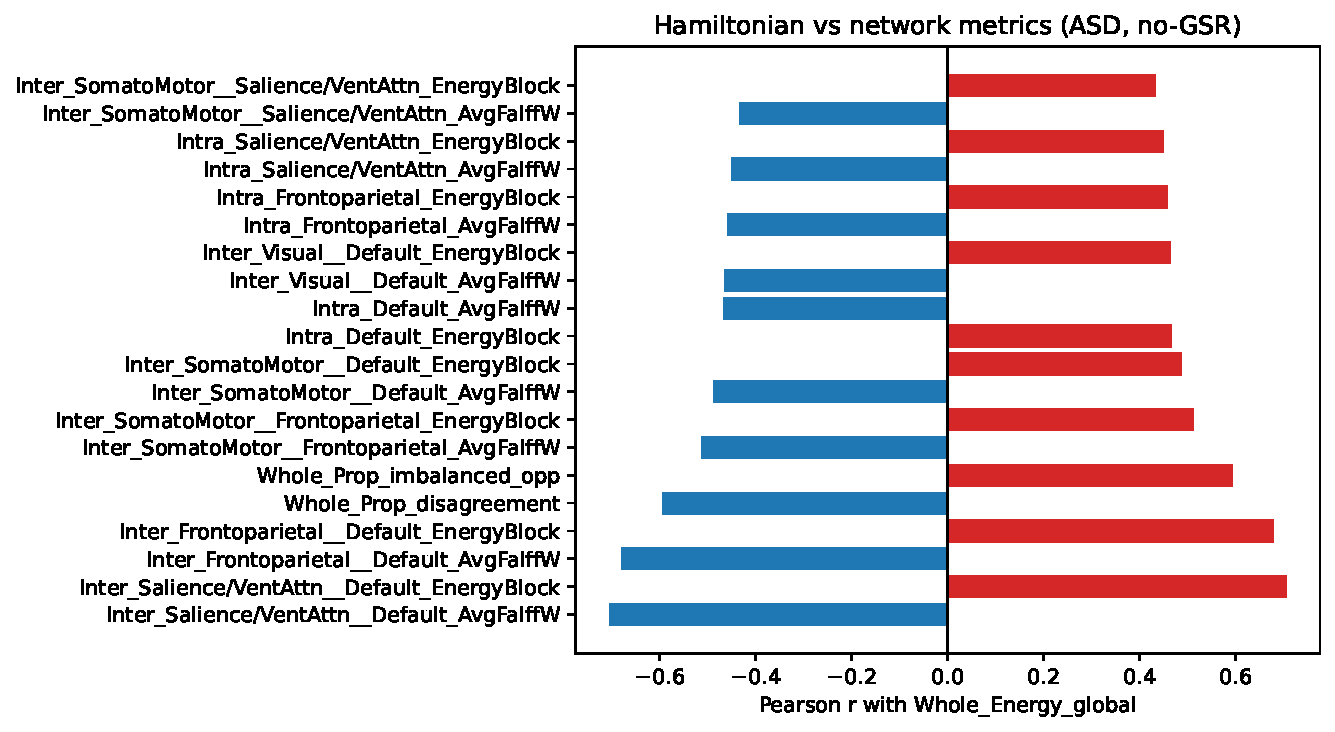
\includegraphics[width=\linewidth]{Images/Hamiltonian_correlates_ASD_GSR.pdf}
  \end{minipage}\hfill
  \begin{minipage}{0.48\textwidth}\centering
    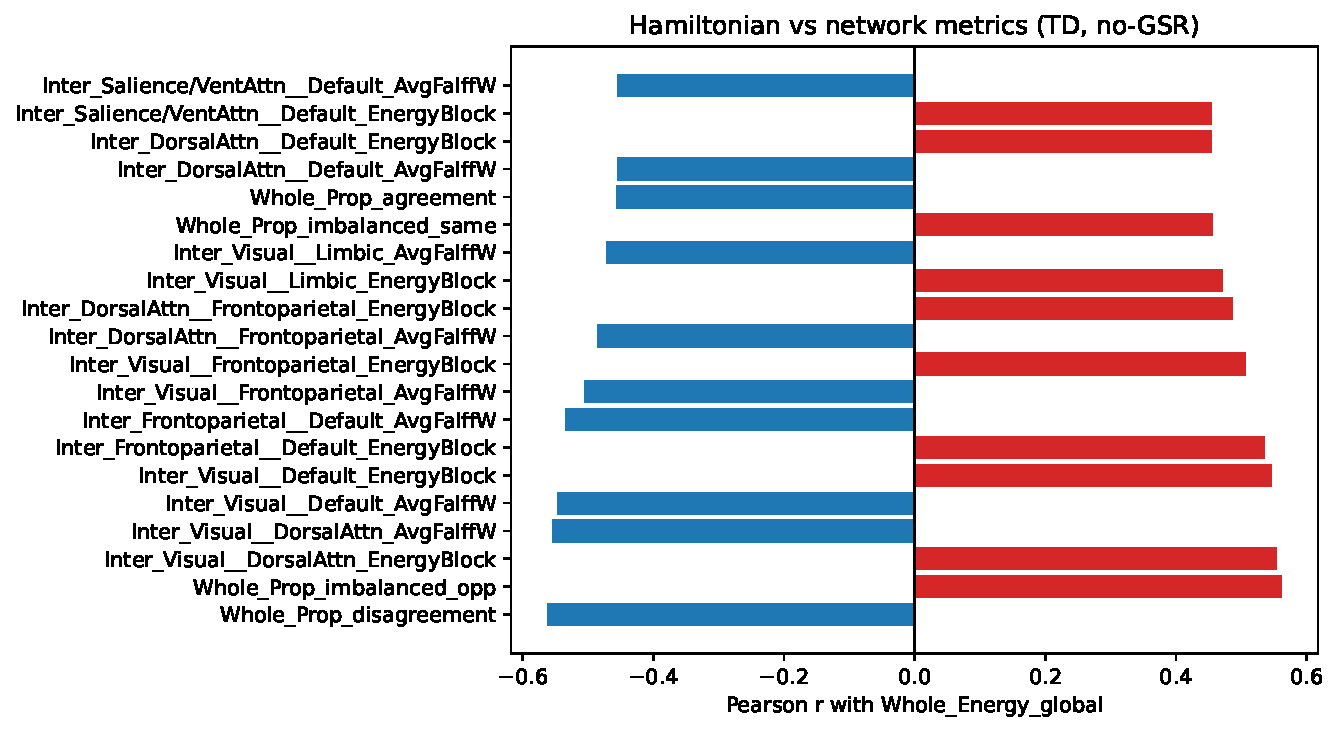
\includegraphics[width=\linewidth]{Images/Hamiltonian_correlates_TD_GSR.pdf}
  \end{minipage}
  \caption{\textbf{Top network metrics correlated with whole-brain coevolutionary energy ($H$),
  GSR pipeline.} Left: ASD group; right: TD group. Provided for comparison with the no-GSR pipeline
  (Fig~\ref{fig:hamil_correlates} and Supplementary Fig~\ref{fig:supp_hamil_td}). Under GSR the
  within-ASD $H$--efficiency correlation is a non-significant trend ($r = -0.20$, $p = 0.075$).}
  \label{fig:supp_hamil_gsr}
\end{figure}

\begin{figure}[H]
  \centering
  \begin{minipage}{0.48\textwidth}\centering
    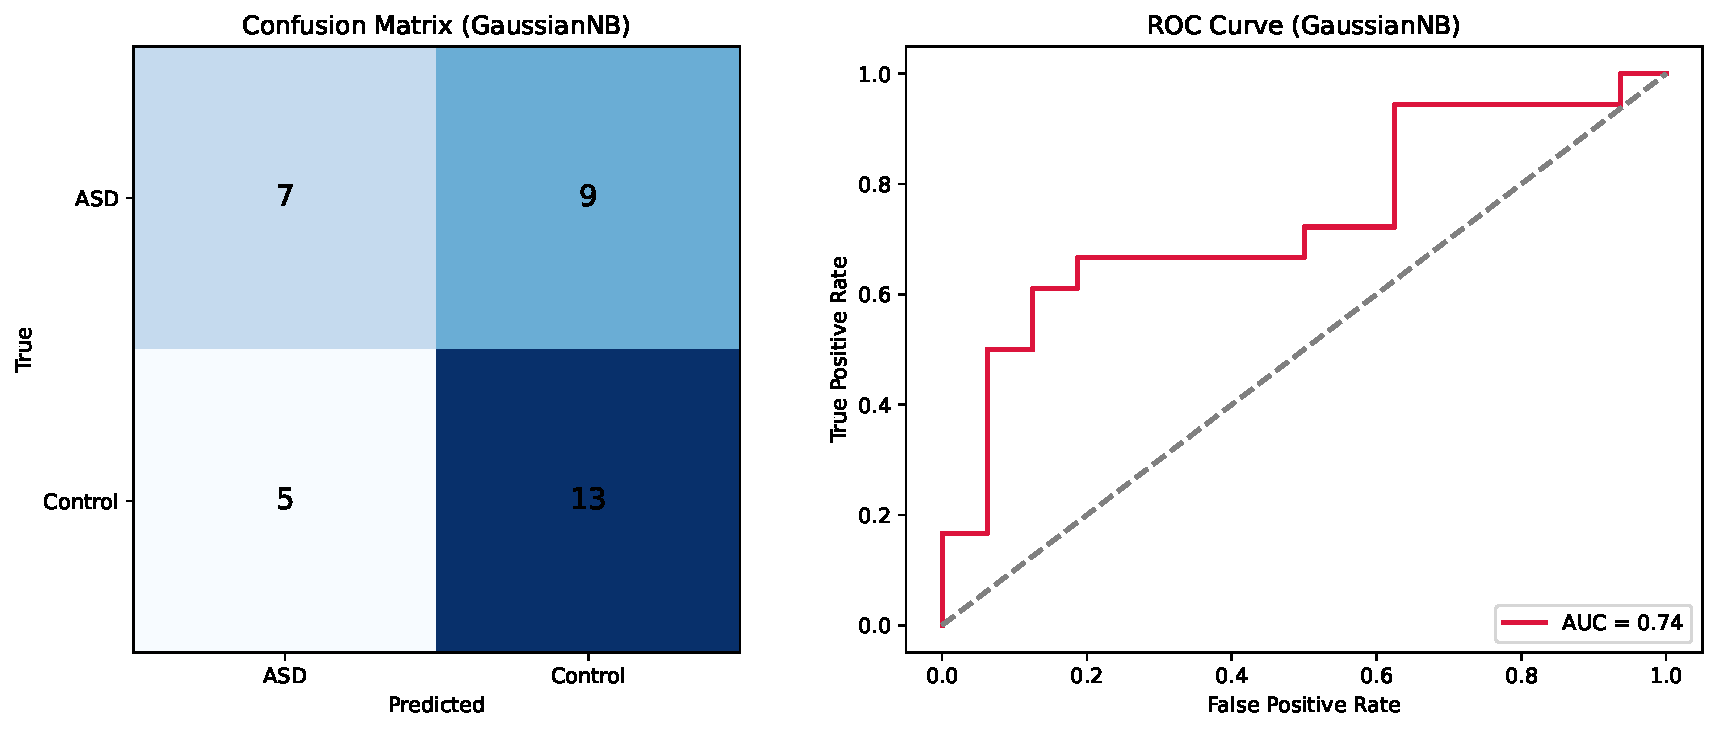
\includegraphics[width=\linewidth]{Images/best_model_GSR.pdf}
  \end{minipage}\hfill
  \begin{minipage}{0.48\textwidth}\centering
    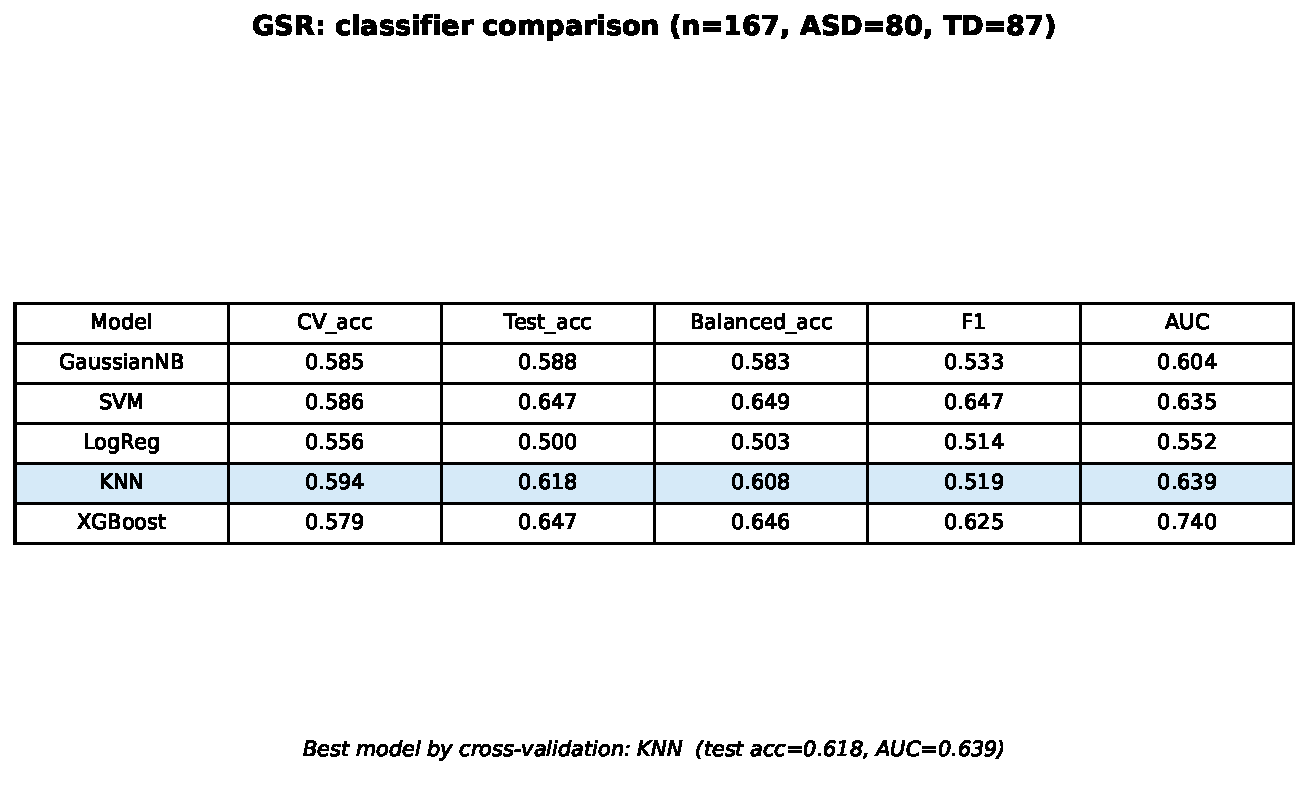
\includegraphics[width=\linewidth]{Images/GSR_results_table.pdf}
  \end{minipage}
  \caption{\textbf{Supervised classification detail, GSR pipeline (harmonized).} Left: best-model
  confusion matrix and ROC. Right: per-model results summary. All models performed at or near chance
  (cross-validated accuracy $0.56$--$0.59$).}
  \label{fig:supp_ml_gsr1}
\end{figure}

\begin{figure}[H]
  \centering
  \begin{minipage}{0.48\textwidth}\centering
    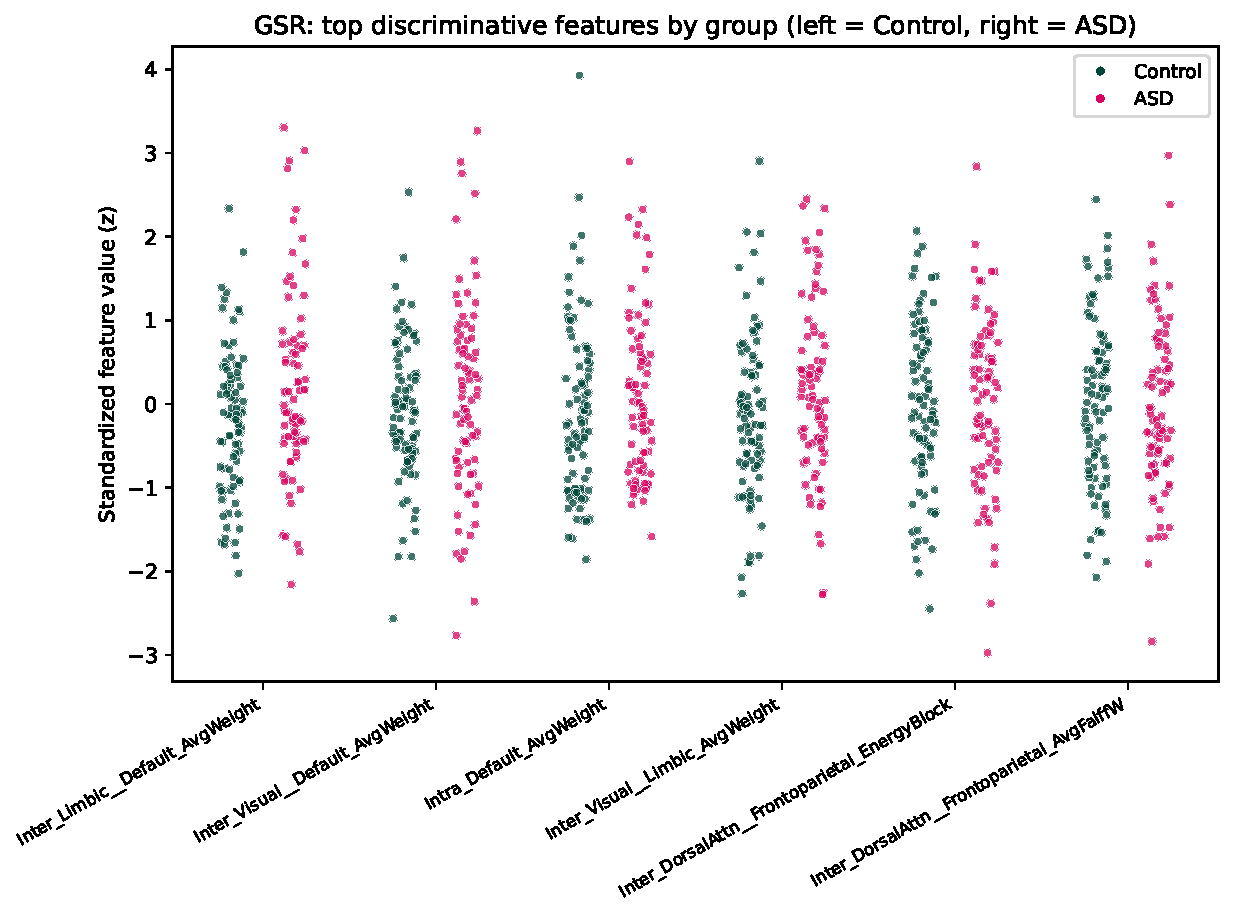
\includegraphics[width=\linewidth]{Images/GSR_top_features.pdf}
  \end{minipage}\hfill
  \begin{minipage}{0.48\textwidth}\centering
    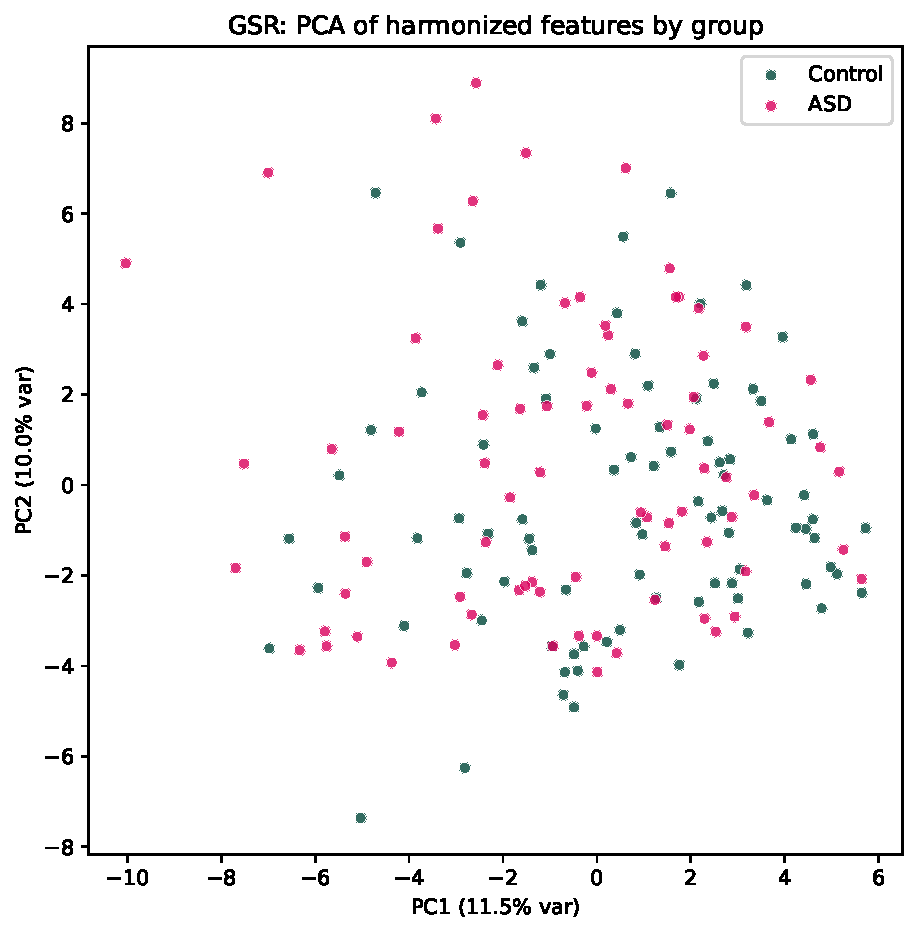
\includegraphics[width=\linewidth]{Images/GSR_pca.pdf}
  \end{minipage}
  \caption{\textbf{Feature ranking and PCA, GSR pipeline (harmonized).} Left: top-ranked features by
  random-forest importance. Right: PCA projection of ASD and TD participants, showing substantial
  overlap consistent with near-chance classification.}
  \label{fig:supp_ml_gsr2}
\end{figure}

\begin{figure}[H]
  \centering
  \begin{minipage}{0.48\textwidth}\centering
    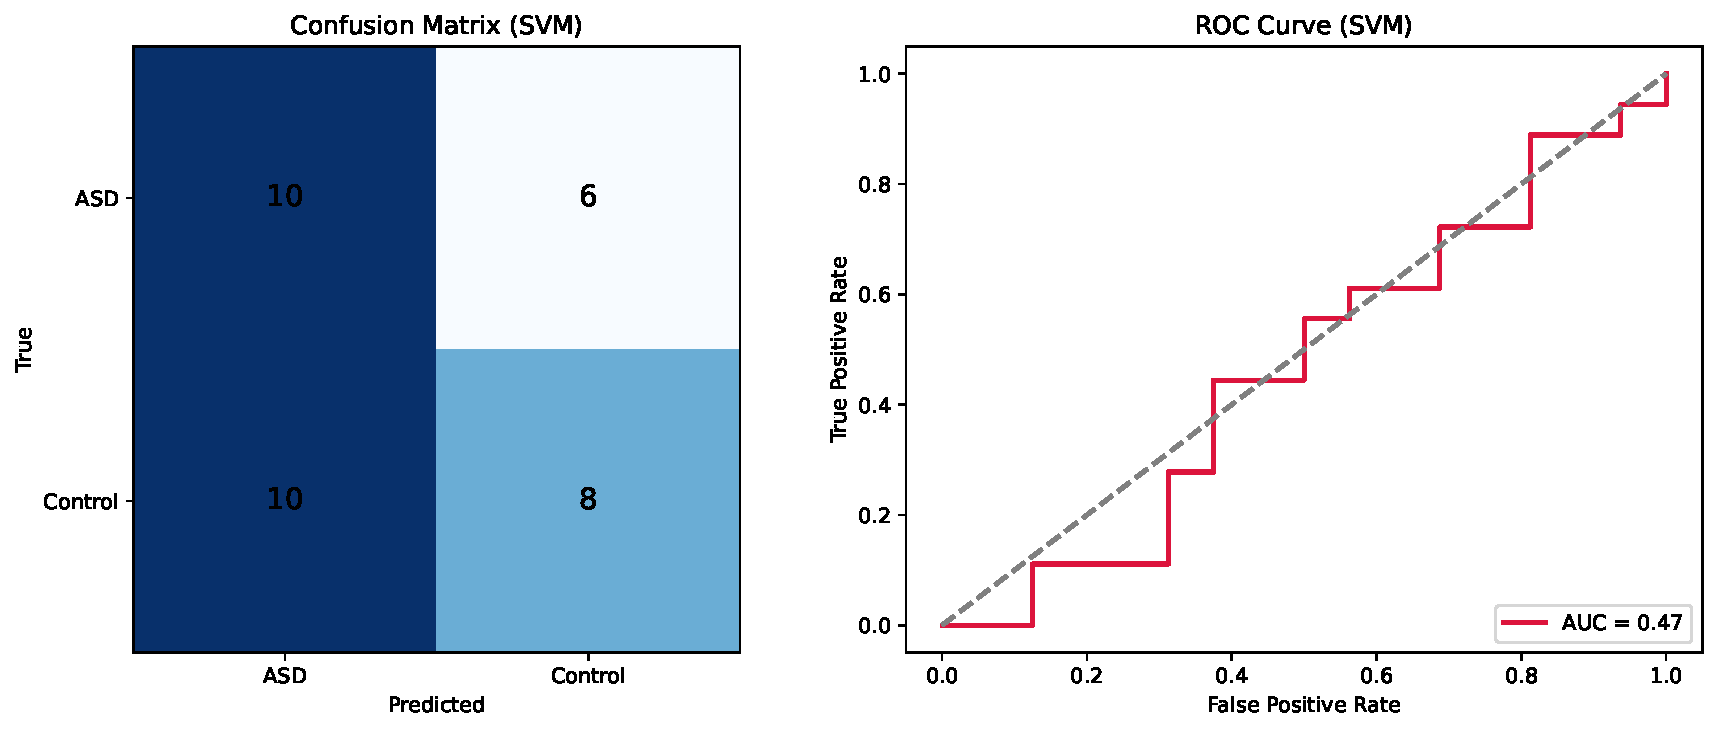
\includegraphics[width=\linewidth]{Images/best_model_noGSR.pdf}
  \end{minipage}\hfill
  \begin{minipage}{0.48\textwidth}\centering
    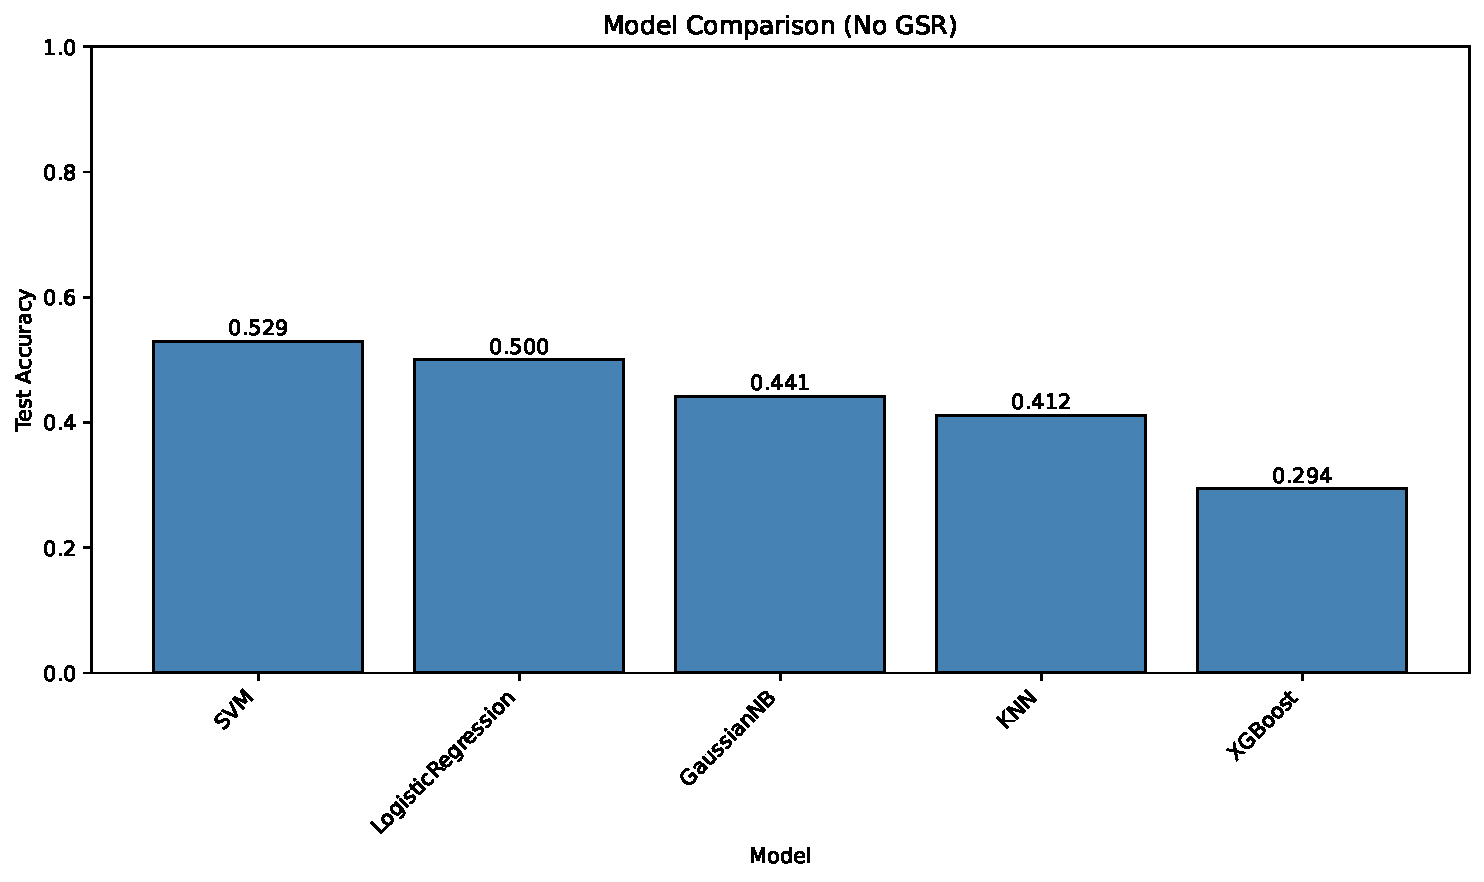
\includegraphics[width=\linewidth]{Images/model_comparison_noGSR.pdf}
  \end{minipage}
  \caption{\textbf{Supervised classification detail, no-GSR pipeline (harmonized).} Left: best-model
  confusion matrix and ROC. Right: comparison of test accuracy across classifiers. Performance is at
  or near chance, as in the GSR pipeline.}
  \label{fig:supp_ml_nogsr1}
\end{figure}

\begin{figure}[H]
  \centering
  \begin{minipage}{0.31\textwidth}\centering
    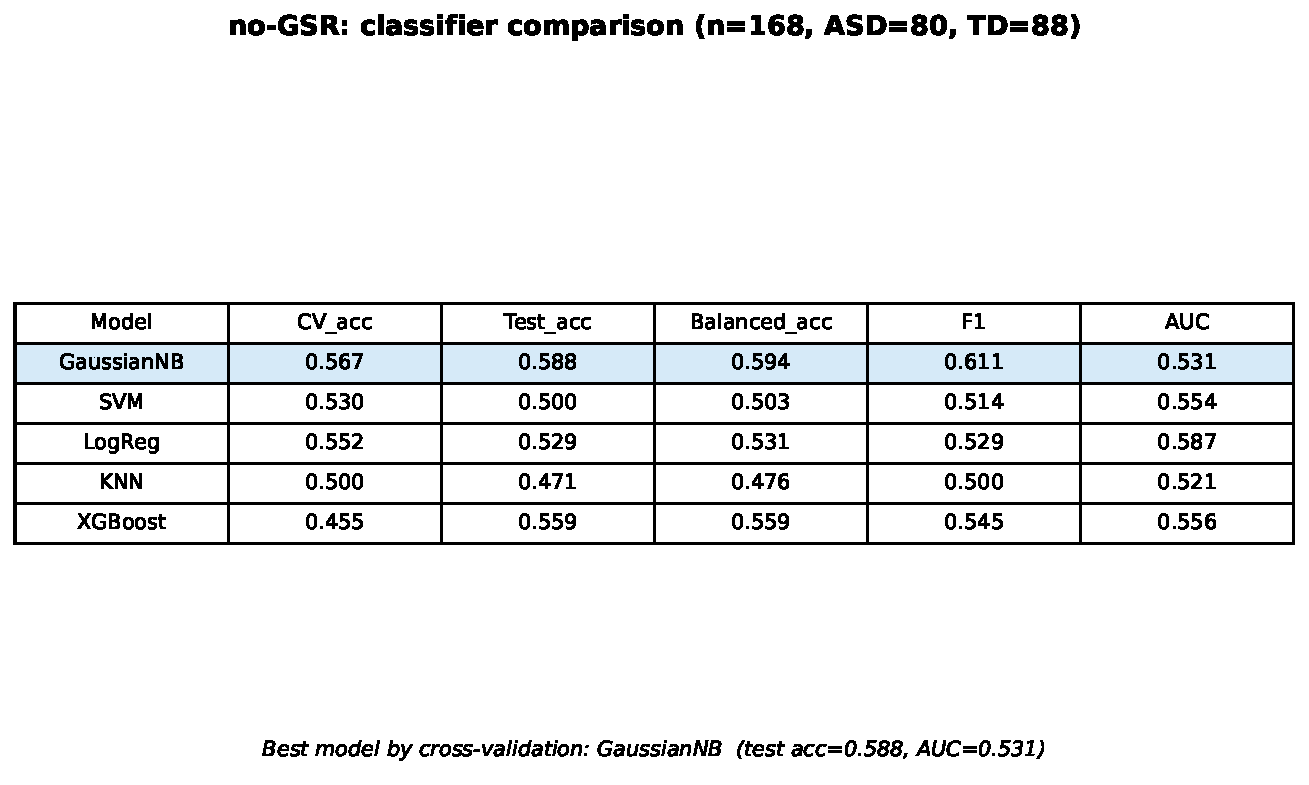
\includegraphics[width=\linewidth]{Images/no-GSR_results_table.pdf}
  \end{minipage}\hfill
  \begin{minipage}{0.31\textwidth}\centering
    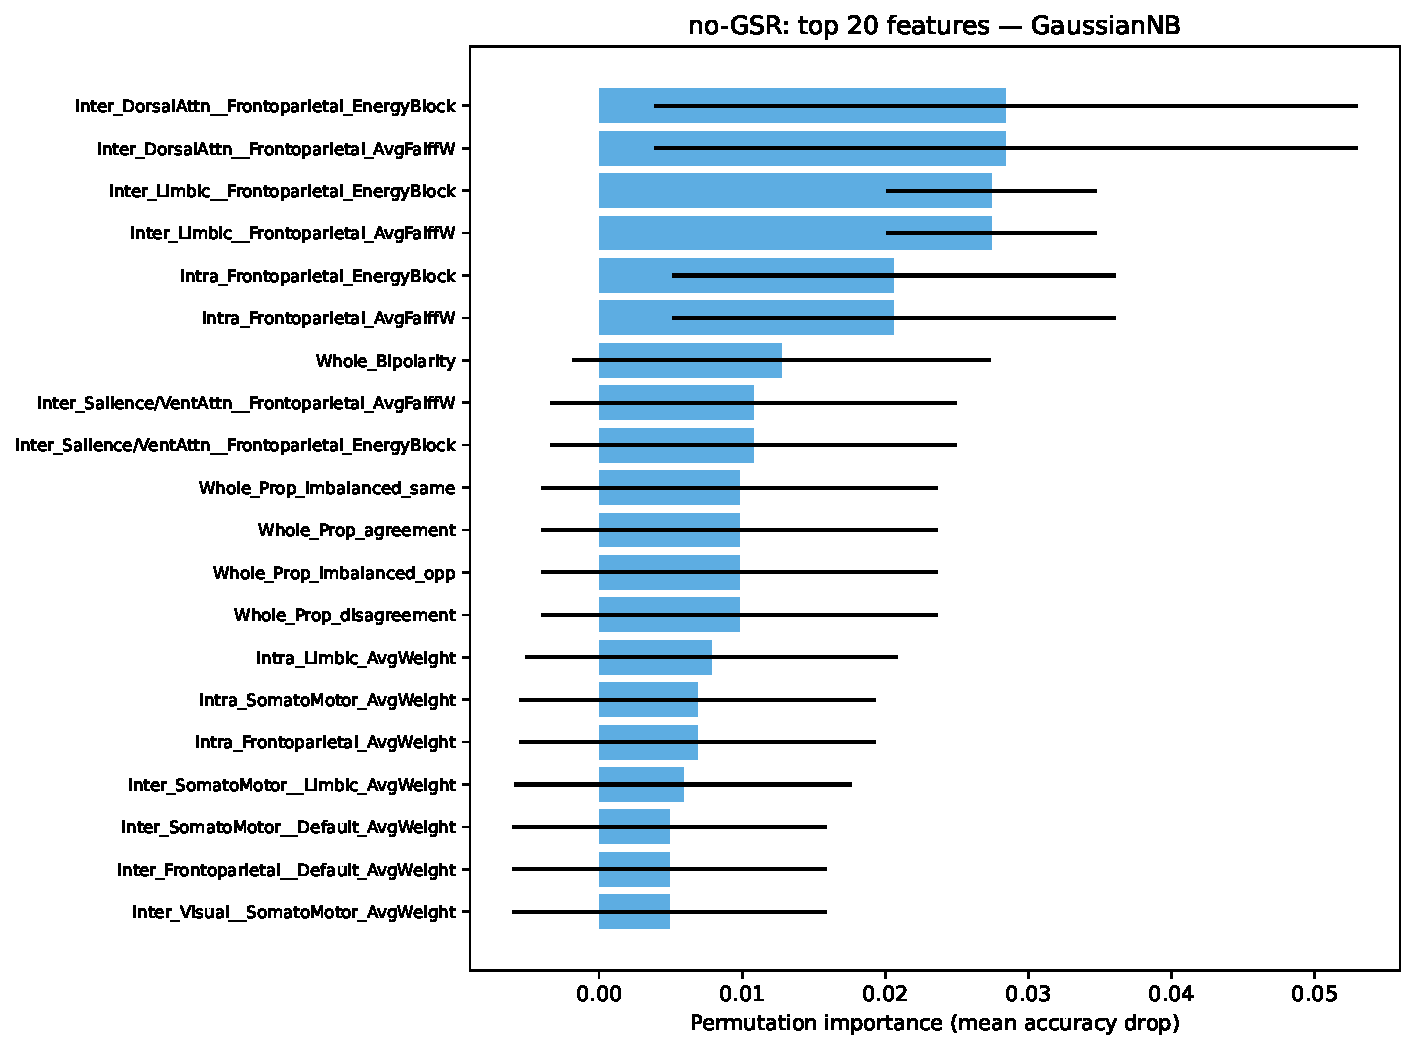
\includegraphics[width=\linewidth]{Images/no-GSR_feature_importance.pdf}
  \end{minipage}\hfill
  \begin{minipage}{0.31\textwidth}\centering
    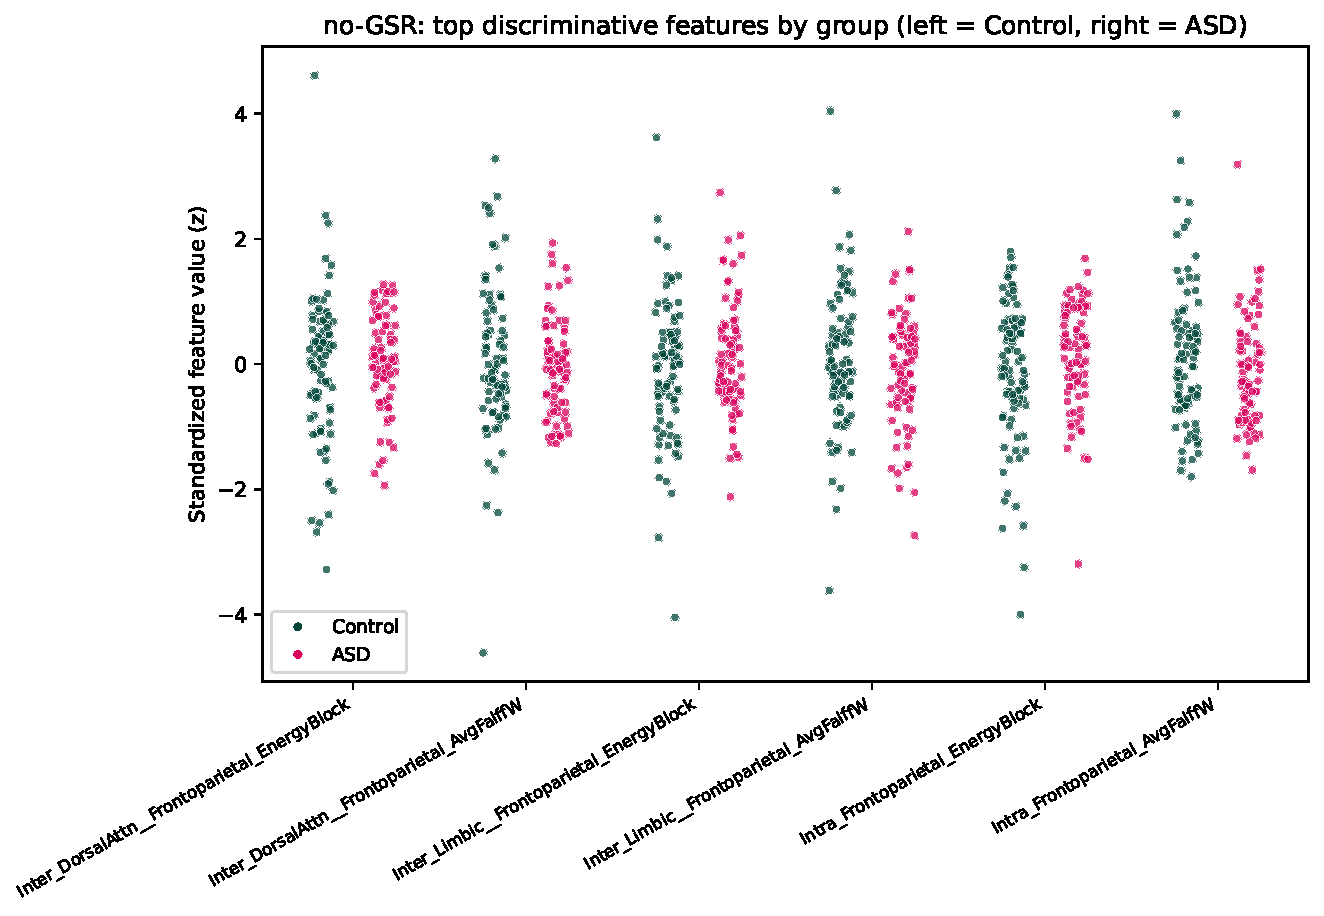
\includegraphics[width=\linewidth]{Images/no-GSR_top_features.pdf}
  \end{minipage}
  \caption{\textbf{No-GSR classification summary, feature importance, and top features
  (harmonized).} Provided for completeness; classification was near chance.}
  \label{fig:supp_ml_nogsr2}
\end{figure}

\begin{figure}[H]
  \centering
  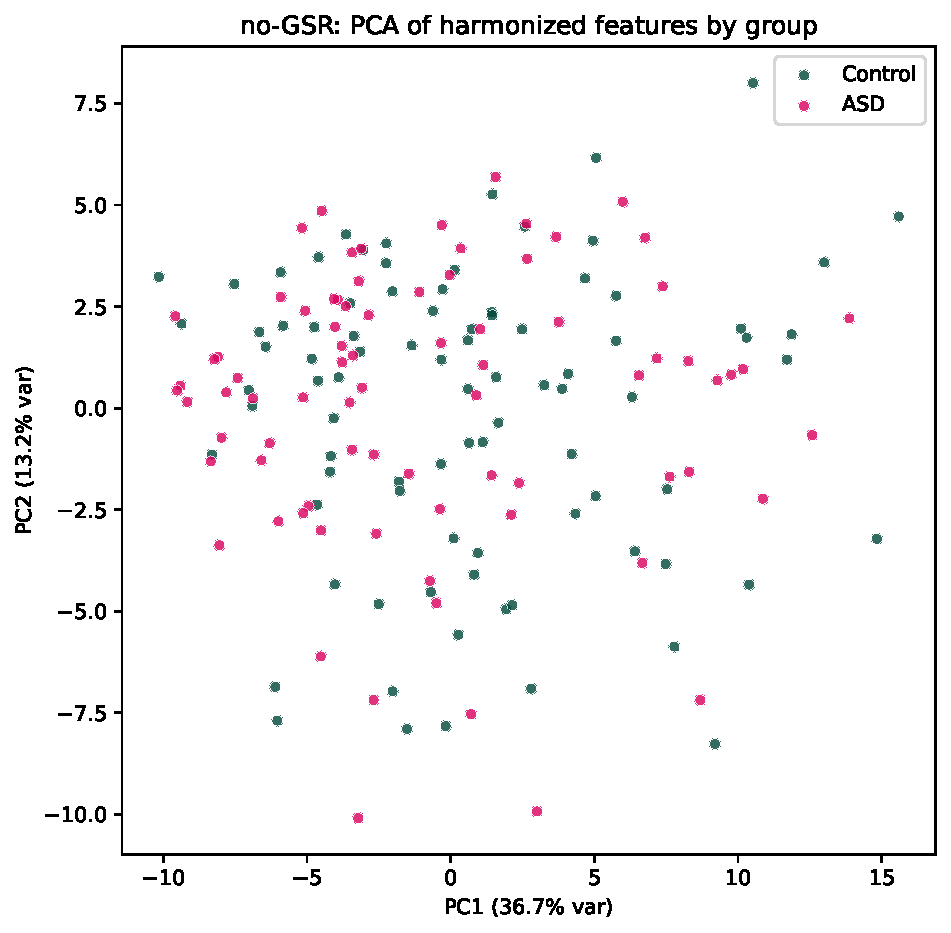
\includegraphics[width=0.5\linewidth]{Images/no-GSR_pca.pdf}
  \caption{\textbf{PCA projection of ASD and TD participants, no-GSR pipeline (harmonized).} The two
  groups overlap substantially, consistent with the absence of FDR-significant group differences.}
  \label{fig:supp_pca_nogsr}
\end{figure}

\begin{figure}[H]
  \centering
  \begin{minipage}{0.48\textwidth}\centering
    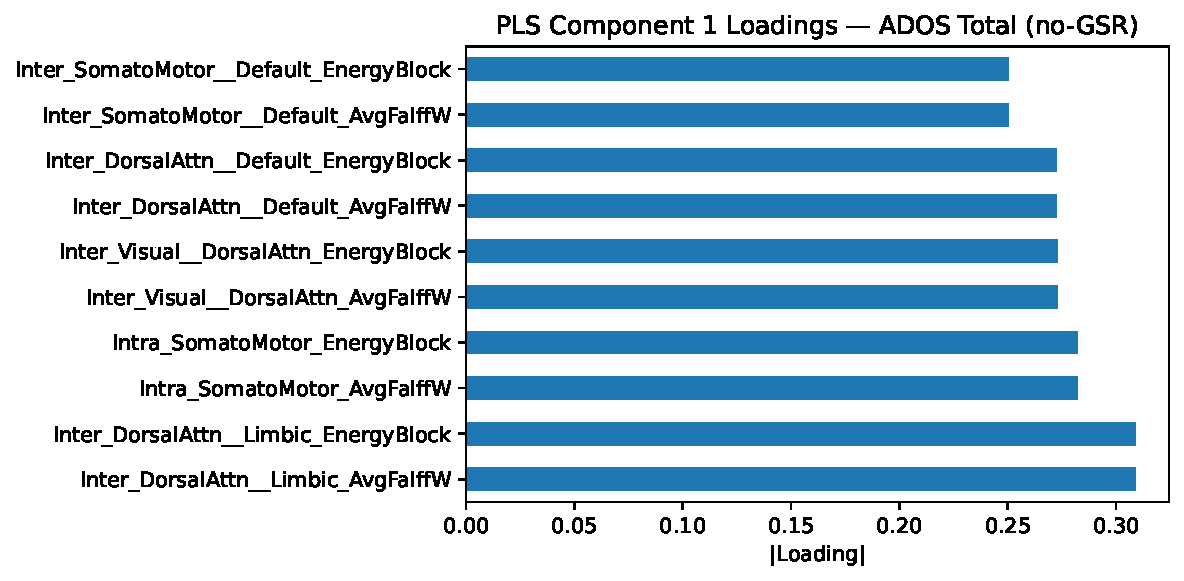
\includegraphics[width=\linewidth]{Images/PLS_loadings_ADOS_Total_GSR.pdf}
  \end{minipage}\hfill
  \begin{minipage}{0.48\textwidth}\centering
    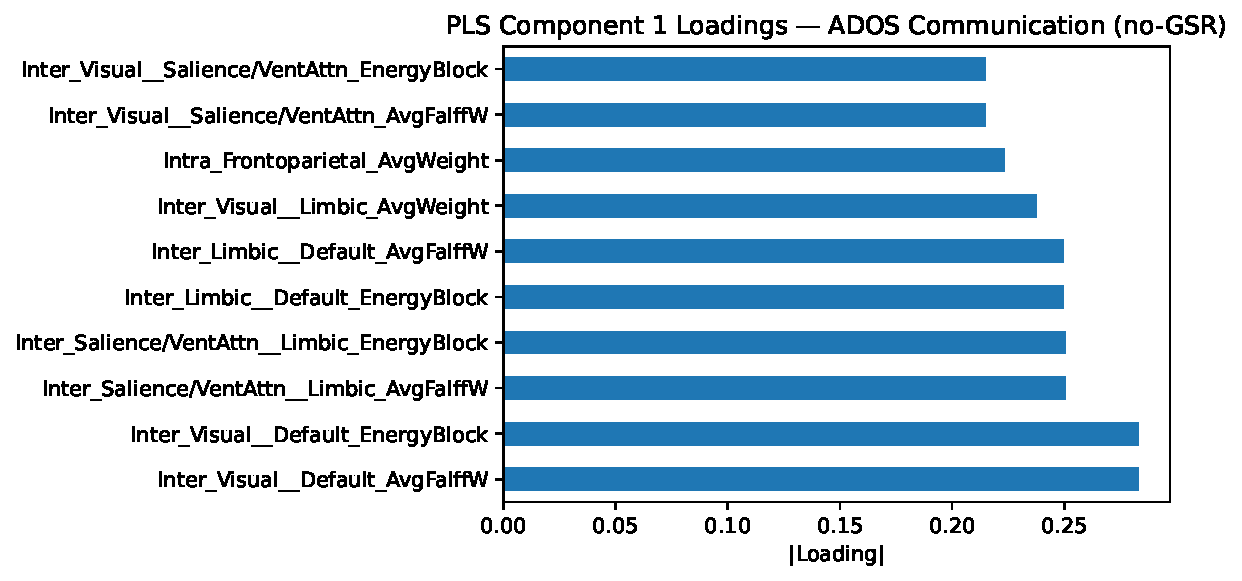
\includegraphics[width=\linewidth]{Images/PLS_loadings_ADOS_Communication_GSR.pdf}
  \end{minipage}
  \caption{\textbf{PLS component-1 loadings (GSR): ADOS Total (left) and ADOS Communication (right).}
  Shown for descriptive purposes only; cross-validated $R^2$ was negative for all scores.}
  \label{fig:supp_pls_gsr1}
\end{figure}

\begin{figure}[H]
  \centering
  \begin{minipage}{0.48\textwidth}\centering
    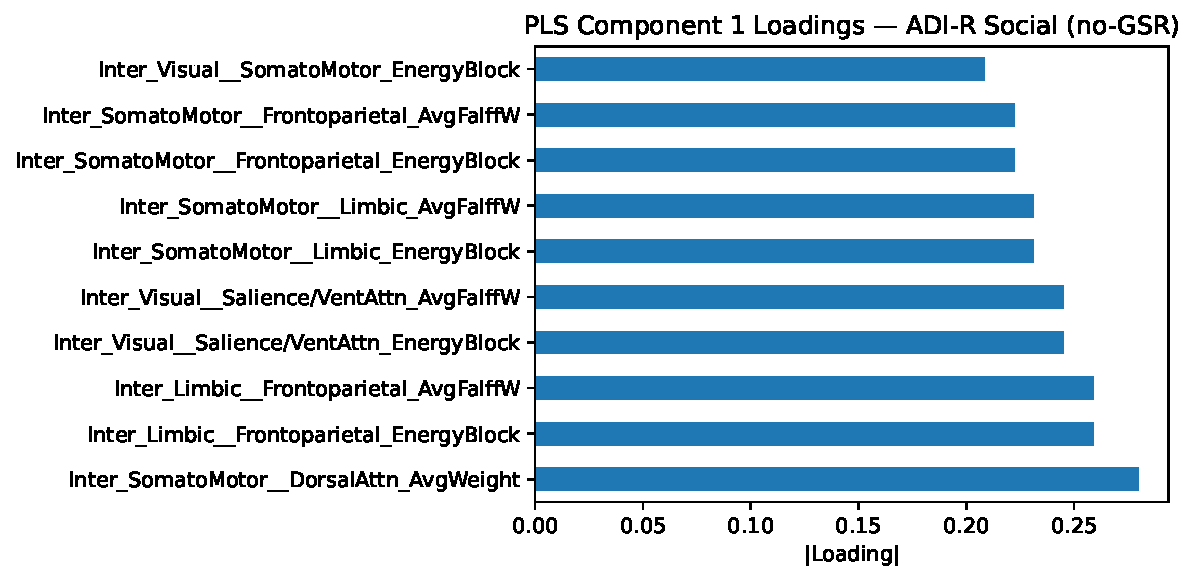
\includegraphics[width=\linewidth]{Images/PLS_loadings_ADI-R_Social_GSR.pdf}
  \end{minipage}\hfill
  \begin{minipage}{0.48\textwidth}\centering
    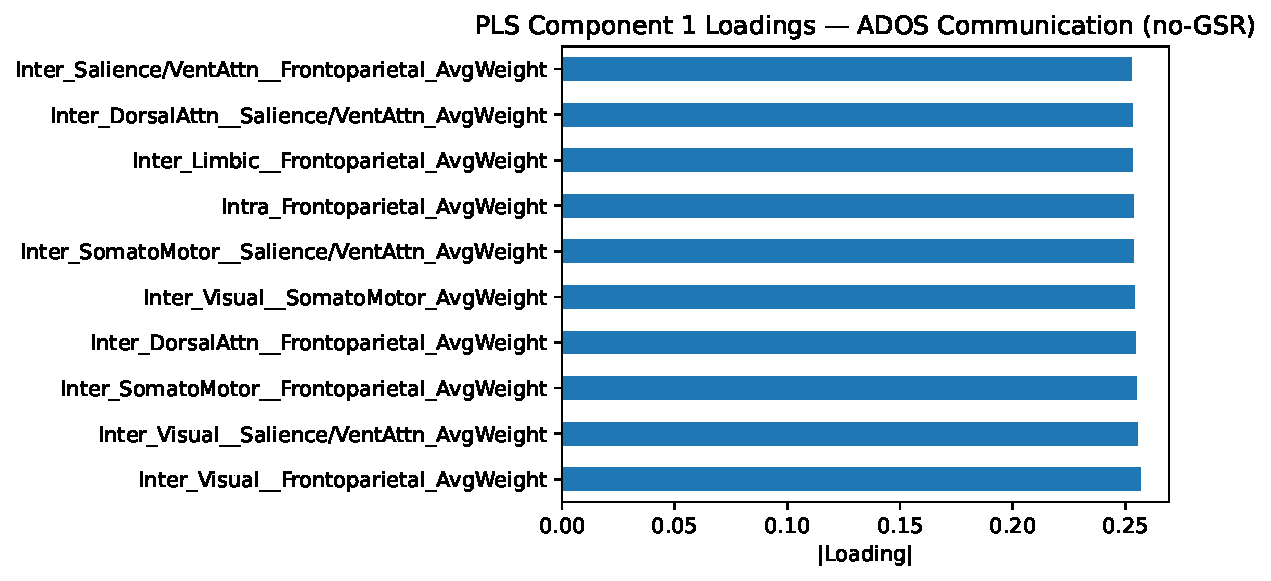
\includegraphics[width=\linewidth]{Images/PLS_loadings_ADOS_Communication_noGSR.pdf}
  \end{minipage}
  \caption{\textbf{PLS component-1 loadings: ADI-R Social (GSR, left) and ADOS Communication
  (no-GSR, right).} Descriptive only.}
  \label{fig:supp_pls_gsr2}
\end{figure}

\begin{figure}[H]
  \centering
  \begin{minipage}{0.48\textwidth}\centering
    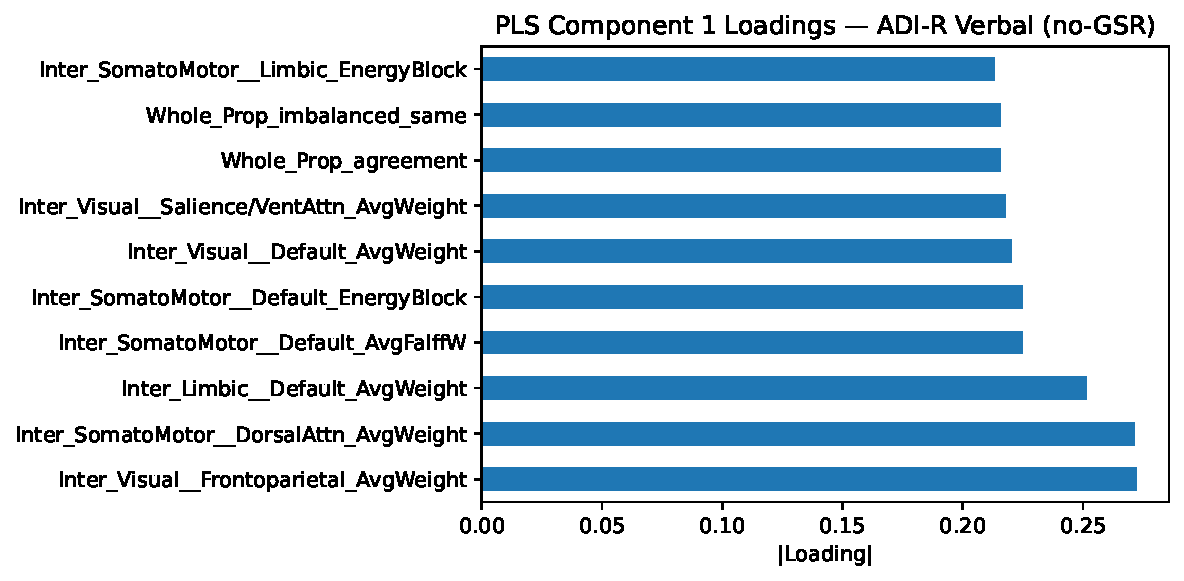
\includegraphics[width=\linewidth]{Images/PLS_loadings_ADI-R_Verbal_GSR.pdf}
  \end{minipage}\hfill
  \begin{minipage}{0.48\textwidth}\centering
    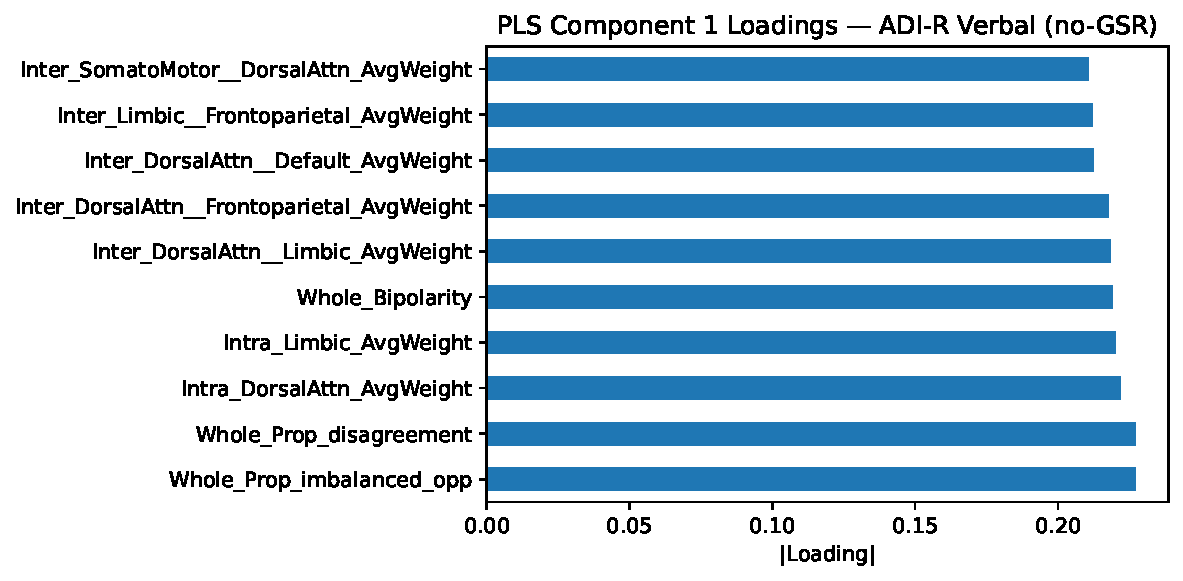
\includegraphics[width=\linewidth]{Images/PLS_loadings_ADI-R_Verbal_noGSR.pdf}
  \end{minipage}
  \caption{\textbf{PLS component-1 loadings for ADI-R Verbal: GSR (left) and no-GSR (right).}
  Descriptive only.}
  \label{fig:supp_pls_verbal}
\end{figure}

\begin{figure}[H]
  \centering
  \begin{minipage}{0.48\textwidth}\centering
    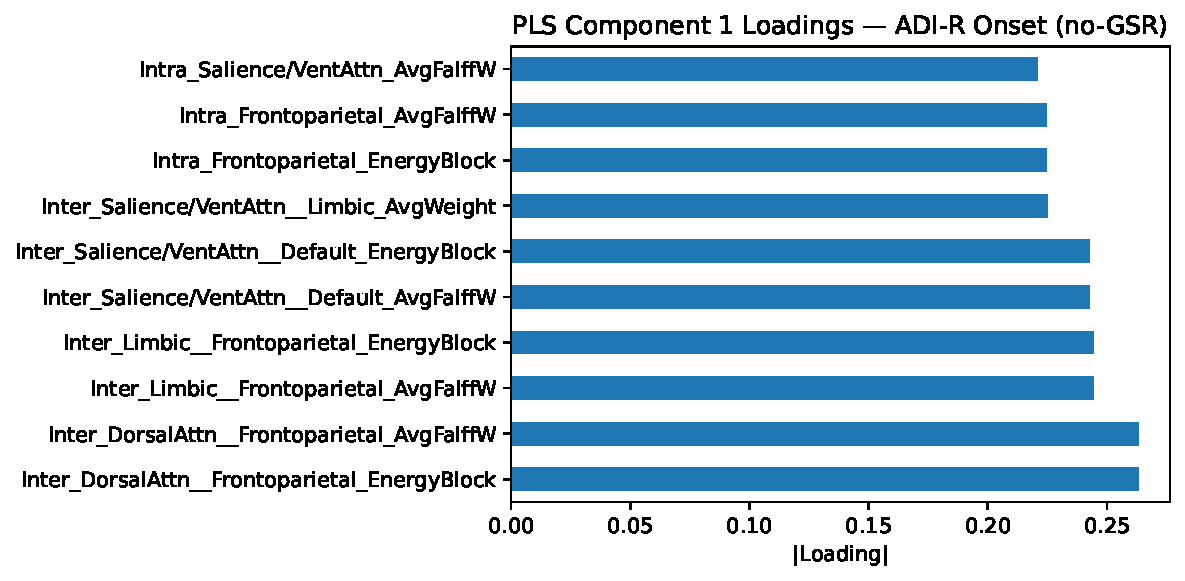
\includegraphics[width=\linewidth]{Images/PLS_loadings_ADI-R_Onset_GSR.pdf}
  \end{minipage}\hfill
  \begin{minipage}{0.48\textwidth}\centering
    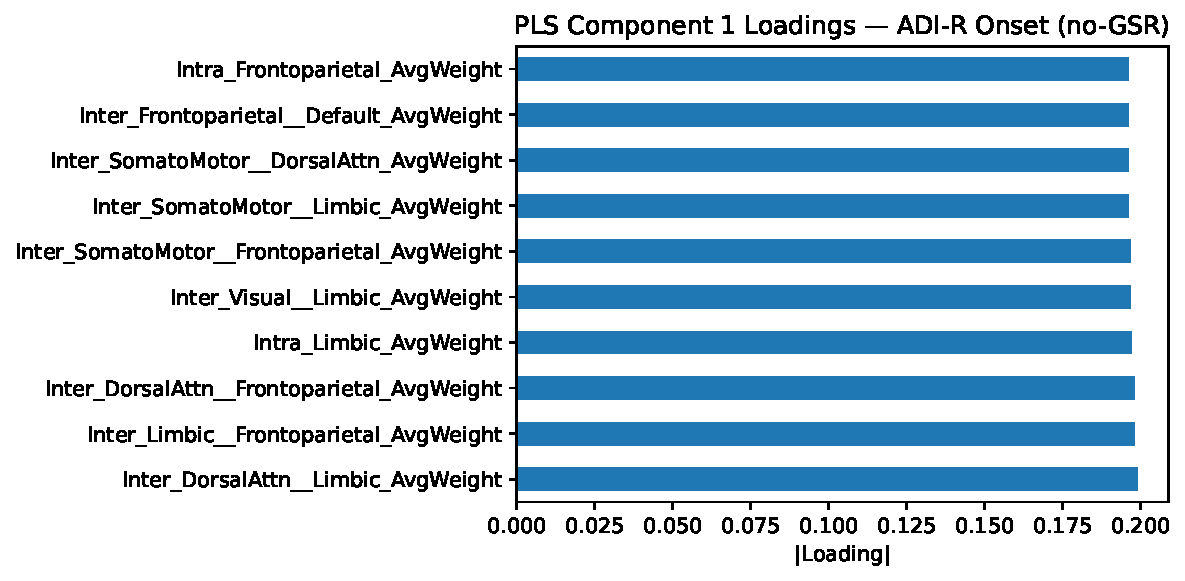
\includegraphics[width=\linewidth]{Images/PLS_loadings_ADI-R_Onset_noGSR.pdf}
  \end{minipage}
  \caption{\textbf{PLS component-1 loadings for ADI-R Onset: GSR (left) and no-GSR (right).}
  Descriptive only.}
  \label{fig:supp_pls_onset}
\end{figure}

\begin{figure}[H]
  \centering
  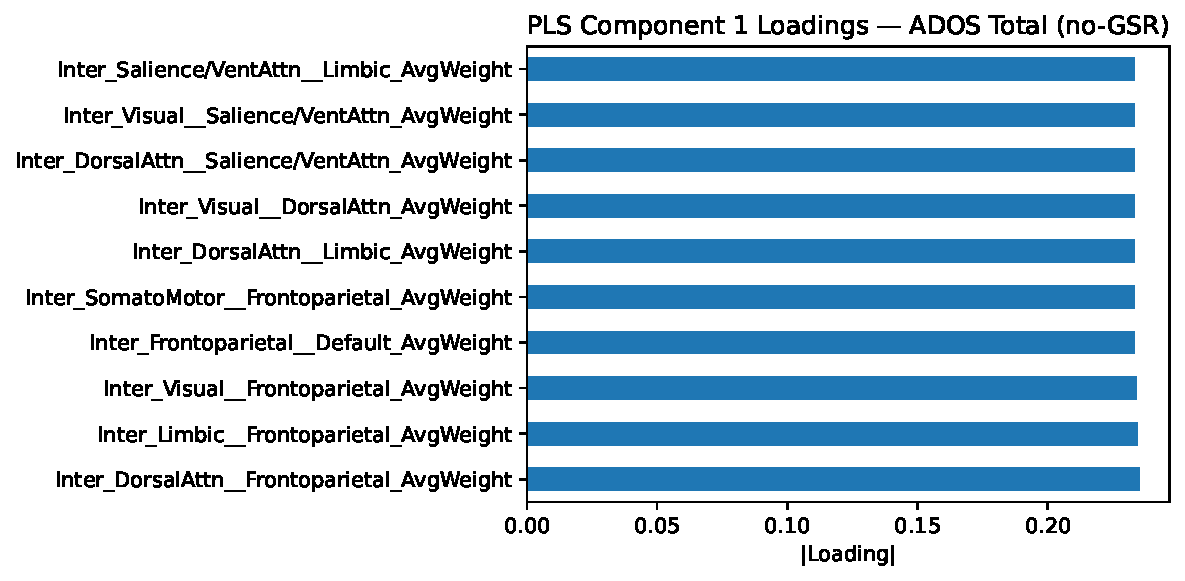
\includegraphics[width=0.7\linewidth]{Images/PLS_loadings_ADOS_Total_noGSR.pdf}
  \caption{\textbf{PLS component-1 loadings for ADOS Total (no-GSR/CompCor).} Top features by
  absolute loading on the first PLS component ($n = 59$ ASD subjects). The cross-validated $R^2$ for
  this component was negative, indicating that PLS does not predict ADOS Total above chance in this
  sample. Shown for descriptive purposes only.}
  \label{fig:supp_pls_ados}
\end{figure}

\begin{figure}[H]
  \centering
  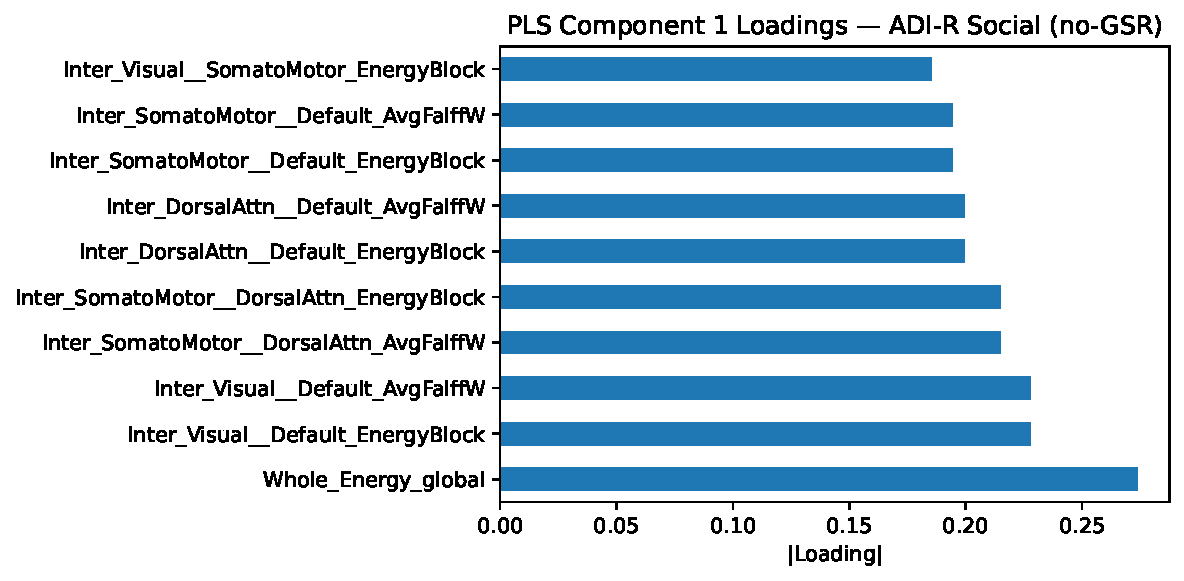
\includegraphics[width=0.7\linewidth]{Images/PLS_loadings_ADI-R_Social_noGSR.pdf}
  \caption{\textbf{PLS component-1 loadings for ADI-R Social Total A (no-GSR/CompCor).} Top features
  by absolute loading on the first PLS component ($n = 32$ ASD subjects; cross-validated
  $R^2 \approx -0.96$). Shown for descriptive purposes only.}
  \label{fig:supp_pls_adir}
\end{figure}

\begin{figure}[H]
  \centering
  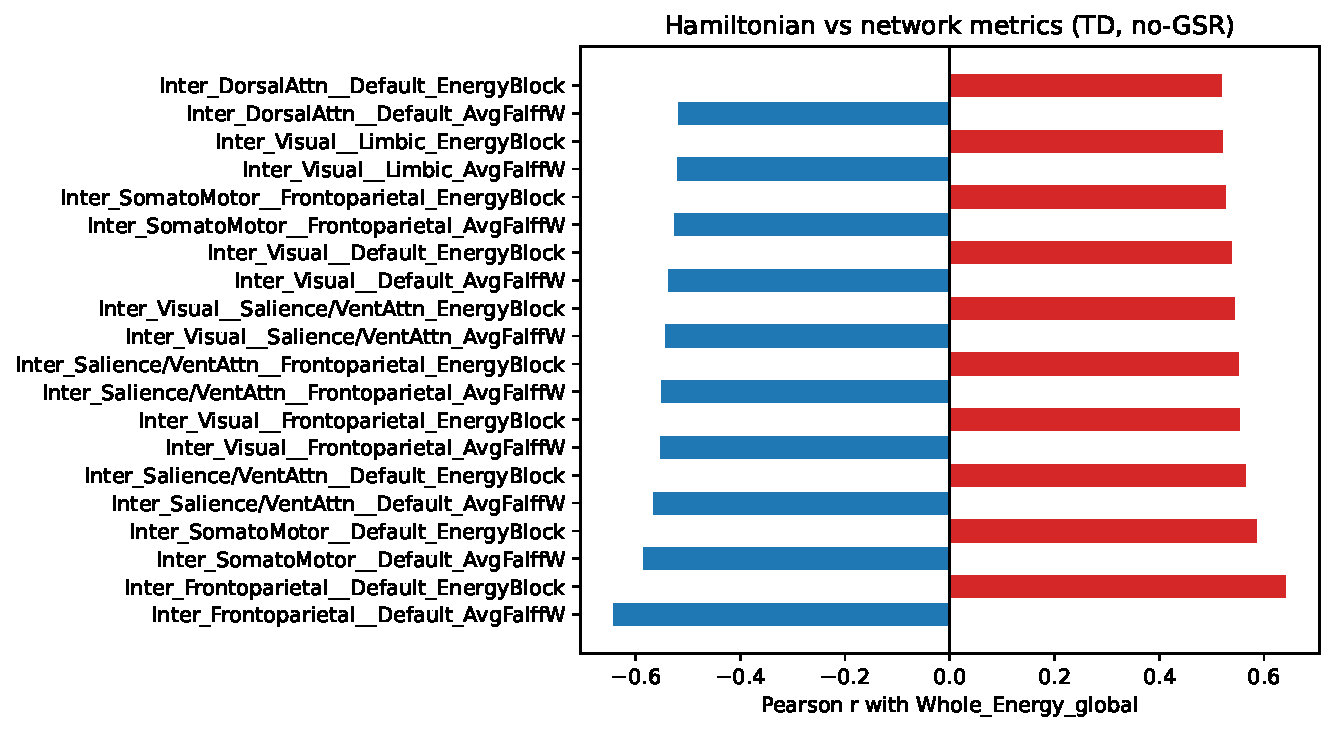
\includegraphics[width=0.95\linewidth]{Images/Hamiltonian_correlates_TD_noGSR.pdf}
  \caption{\textbf{Top 20 network metrics most strongly correlated with whole-brain coevolutionary
  energy ($H$) within the TD group (no-GSR pipeline).} Red bars indicate positive correlations
  (EnergyBlock features); blue bars indicate negative correlations. Compare with
  Fig~\ref{fig:hamil_correlates} (ASD group). The efficiency--$H$ correlation is weaker and
  non-significant in TD ($r = -0.17$, $p = 0.12$) than in ASD ($r = -0.33$, FDR $p = 0.005$),
  suggesting that the within-group stability--efficiency association is more pronounced in autistic
  individuals (an exploratory, pipeline-dependent observation).}
  \label{fig:supp_hamil_td}
\end{figure}

\begin{table}[htbp]
\centering
\caption{\textbf{Full list of nominally significant feature--clinical score correlations
(uncorrected $p < 0.05$).} The comprehensive analysis tested 460 correlations (92 features
$\times$ 8 clinical scores). This table lists all 64 pairs that reached uncorrected significance
for either Pearson or Spearman tests. None survived FDR correction. Sample sizes vary due to
missing clinical data. The sign of $r$ is provided explicitly to allow unambiguous directional
interpretation. A negative $r$ for Whole\_Energy\_global means more negative $H$ (more stable)
is associated with higher ADOS (more severe); see main text for full directional interpretation.}
\label{tab:supp_corr_sig}

\scriptsize

\begin{tabularx}{\textwidth}{
>{\raggedright\arraybackslash}p{5cm}
>{\raggedright\arraybackslash}p{3cm}
ccccc
}
\toprule
\textbf{Feature} &
\textbf{Clinical Score} &
\textbf{$n$} &
\textbf{$r$} &
\textbf{$p$} &
\textbf{$\rho$} &
\textbf{$p^{\rho}$} \\
\midrule

\seqsplit{Intra\_Salience/VentAttn\_AvgWeight}
& \seqsplit{ADOS\_COMM}
& 71 & $-$0.41 & 0.0004 & $-$0.42 & 0.0002 \\

\seqsplit{Intra\_Default\_AvgWeight}
& \seqsplit{ADOS\_COMM}
& 71 & $-$0.39 & 0.0007 & $-$0.40 & 0.0006 \\

\seqsplit{Inter\_DorsalAttn\_\_Default\_AvgWeight}
& \seqsplit{ADOS\_COMM}
& 71 & $+$0.36 & 0.0019 & $+$0.36 & 0.0018 \\

\seqsplit{Intra\_Default\_AvgWeight}
& \seqsplit{ADOS\_TOTAL}
& 81 & $-$0.34 & 0.0022 & $-$0.33 & 0.0027 \\

\seqsplit{Intra\_Salience/VentAttn\_AvgWeight}
& \seqsplit{ADOS\_TOTAL}
& 81 & $-$0.33 & 0.0029 & $-$0.32 & 0.0032 \\

\seqsplit{Intra\_Default\_AvgWeight}
& \seqsplit{ADOS\_SOCIAL}
& 71 & $-$0.32 & 0.0072 & $-$0.30 & 0.0104 \\

\seqsplit{Inter\_DorsalAttn\_\_Default\_AvgWeight}
& \seqsplit{ADOS\_TOTAL}
& 81 & $+$0.29 & 0.0084 & $+$0.30 & 0.0061 \\

\seqsplit{Inter\_Salience/VentAttn\_\_Default\_AvgWeight}
& \seqsplit{ADOS\_COMM}
& 71 & $+$0.31 & 0.0094 & $+$0.28 & 0.0167 \\

\seqsplit{Inter\_DorsalAttn\_\_Salience/VentAttn\_EnergyBlock}
& \seqsplit{ADI\_R\_SOCIAL\_TOTAL\_A}
& 39 & $-$0.41 & 0.0099 & $-$0.39 & 0.0147 \\

\seqsplit{Inter\_DorsalAttn\_\_Salience/VentAttn\_AvgFalffW}
& \seqsplit{ADI\_R\_SOCIAL\_TOTAL\_A}
& 39 & $+$0.41 & 0.0104 & $+$0.38 & 0.0159 \\

\seqsplit{Inter\_Salience/VentAttn\_\_Default\_AvgWeight}
& \seqsplit{ADOS\_TOTAL}
& 81 & $+$0.28 & 0.0104 & $+$0.28 & 0.0129 \\

\seqsplit{Inter\_Salience/VentAttn\_\_Default\_AvgWeight}
& \seqsplit{ADOS\_SOCIAL}
& 71 & $+$0.30 & 0.0110 & $+$0.29 & 0.0154 \\

\seqsplit{Inter\_DorsalAttn\_\_Default\_AvgWeight}
& \seqsplit{ADOS\_SOCIAL}
& 71 & $+$0.29 & 0.0131 & $+$0.30 & 0.0104 \\

\seqsplit{Inter\_Visual\_\_Limbic\_AvgFalffW}
& \seqsplit{ADI\_R\_ONSET\_TOTAL\_D}
& 36 & $+$0.40 & 0.0155 & $+$0.43 & 0.0092 \\

\seqsplit{Whole\_Energy\_global}
& \seqsplit{ADOS\_TOTAL}
& 81 & $-$0.26 & 0.0169 & $-$0.24 & 0.0306 \\

\seqsplit{Inter\_Visual\_\_Limbic\_EnergyBlock}
& \seqsplit{ADI\_R\_ONSET\_TOTAL\_D}
& 36 & $-$0.39 & 0.0175 & $-$0.42 & 0.0101 \\

\seqsplit{Intra\_Salience/VentAttn\_AvgWeight}
& \seqsplit{ADOS\_SOCIAL}
& 71 & $-$0.28 & 0.0202 & $-$0.26 & 0.0318 \\

\seqsplit{Intra\_DorsalAttn\_AvgWeight}
& \seqsplit{ADOS\_COMM}
& 71 & $-$0.27 & 0.0209 & $-$0.32 & 0.0073 \\

\multicolumn{7}{c}{\textit{... 46 additional rows (see online supplementary data) ...}} \\

\bottomrule
\end{tabularx}

\begin{flushleft}
\footnotesize
Note: The full table with all 64 nominally significant correlations is available in the online
supplementary data file \texttt{significant\_uncorrected.csv}. FDR-corrected $p$-values ranged
from 0.17 to 0.87; none reached significance at $q < 0.05$. The sign of $r$ is shown explicitly
throughout; abbreviations: COMM = Communication, SOC = Social, Sal/VA = Salience/VentAttn,
DA = DorsalAttn, Def = Default.
\end{flushleft}

\end{table}

\begin{table}[htbp]
\centering
\caption{\textbf{Summary statistics for the comprehensive correlation analysis.} Overview of the
feature--clinical score correlation analysis, including sample sizes, number of tests, and
significance thresholds.}
\label{tab:supp_corr_full}
\small
\begin{tabular}{lc}
\toprule
\textbf{Parameter} & \textbf{Value} \\
\midrule
Total network features tested & 90 \\
Clinical scores tested & 8 \\
Total correlation tests & 460 \\
Subjects with matched data & 85 \\
Sample size range (per clinical score) & 36--81 \\
\midrule
\multicolumn{2}{l}{\textit{Clinical scores and sample sizes:}} \\
\quad ADOS\_TOTAL & $n = 81$ \\
\quad ADOS\_COMM & $n = 71$ \\
\quad ADOS\_SOCIAL & $n = 71$ \\
\quad ADOS\_STEREO\_BEHAV & $n = 63$ \\
\quad ADI\_R\_SOCIAL\_TOTAL\_A & $n = 39$ \\
\quad ADI\_R\_VERBAL\_TOTAL\_BV & $n = 39$ \\
\quad ADI\_RRB\_TOTAL\_C & $n = 39$ \\
\quad ADI\_R\_ONSET\_TOTAL\_D & $n = 36$ \\
\midrule
Nominally significant (uncorrected $p < 0.05$) & 64 (8.9\%) \\
FDR-significant ($q < 0.05$) & 0 (0\%) \\
Strongest Pearson $r$ (signed) & $-0.41$ \\
Smallest uncorrected $p$ & 0.0004 \\
\midrule
\multicolumn{2}{l}{\textit{PLS cross-validated $R^2$ (all scores, all components):}} \\
\quad Range & $-1.94$ to $-0.11$ \\
\quad All values negative & Yes (no above-chance prediction) \\
\bottomrule
\end{tabular}
\end{table}

\end{document}

\end{document}
